\chapter{Funciones medibles. Integral de Lebesgue}

\section{Aplicaciones medibles}

\begin{definicion}{Aplicación medible}{def:aplicacion_medible}
Dados dos espacios medibles $(\Omega_1, \mathcal{G}_1)$ y $(\Omega_2, \mathcal{G}_2)$, la aplicación $X : \Omega_1 \to \Omega_2$ es \textbf{medible} si y solo si para todo conjunto medible $B \in \mathcal{G}_2$ se tiene que su imagen inversa $X^{-1}(B)$ pertenece a $\mathcal{G}_1$, es decir:
\[
    X^{-1}(\mathcal{G}_2) \subseteq \mathcal{G}_1
\]
Denotaremos esto escribiendo $X : (\Omega_1, \mathcal{G}_1) \to (\Omega_2, \mathcal{G}_2)$.
\end{definicion}

\paragraph{Notación de antiimágenes:}
Para cada suceso $B \in \mathcal{G}_2$, el elemento imagen inversa se denota indistintamente por:
\[
    X^{-1}(B) = \{ \omega_1 \in \Omega_1 \mid X(\omega_1) \in B \} \equiv \{ X \in B \}
\]

% ------------------------------------------------------------------------------
\begin{proposicion}{$\sigma$-álgebra generada por una aplicación}{prop12}
Sea $X : \Omega_1 \to \Omega_2$ una aplicación y $(\Omega_2, \mathcal{G}_2)$ un espacio medible. La mínima $\sigma$-álgebra sobre $\Omega_1$ respecto de la cual $X$ es medible viene dada por:
\[
    X^{-1}(\mathcal{G}_2) = \{ A \subseteq \Omega_1 \mid \exists B \in \mathcal{G}_2 \text{ tal que } A = X^{-1}(B) \}
\]
A esta estructura se la denota por $\sigma(X) \equiv X^{-1}(\mathcal{G}_2)$ y se la llama $\sigma$-álgebra generada por $X$.
\end{proposicion}

\begin{demostracion}
Procedemos en dos pasos:
\begin{enumerate}[label=\arabic*.]
    \item \textit{Estructura de $\sigma$-álgebra de $X^{-1}(\mathcal{G}_2)$:}
    Dado que $\mathcal{G}_2$ es una $\sigma$-álgebra sobre $\Omega_2$, por las propiedades fundamentales de la imagen inversa, la colección $X^{-1}(\mathcal{G}_2)$ hereda automáticamente todas las propiedades de $\sigma$-álgebra sobre $\Omega_1$.
    
    \item \textit{Minimalidad de $X^{-1}(\mathcal{G}_2)$:}
    Para todo $B \in \mathcal{G}_2$, $X^{-1}(B) \in X^{-1}(\mathcal{G}_2)$, por lo que $X$ es trivialmente medible respecto a $X^{-1}(\mathcal{G}_2)$ y $\mathcal{G}_2$.
    
    Sea ahora $\mathcal{G}_1$ cualquier otra $\sigma$-álgebra sobre $\Omega_1$ respecto de la cual $X$ sea medible. Por definición de medibilidad, dado un conjunto arbitrario $A \in X^{-1}(\mathcal{G}_2)$, existe $B \in \mathcal{G}_2$ tal que $A = X^{-1}(B) \in \mathcal{G}_1$. En consecuencia, $X^{-1}(\mathcal{G}_2) \subseteq \mathcal{G}_1$, lo que demuestra la minimalidad.
\end{enumerate}
\end{demostracion}

% ------------------------------------------------------------------------------
\begin{corolario}{Criterio de medibilidad por clases generadoras}{cor2}
Una aplicación $X : (\Omega_1, \mathcal{G}_1) \to (\Omega_2, \mathcal{G}_2)$ es medible si y solo si existe una clase de subconjuntos $\mathcal{C}$ de $\Omega_2$ tal que genera la $\sigma$-álgebra $\mathcal{G}_2$ ($\sigma(\mathcal{C}) = \mathcal{G}_2$) y satisface:
\[
    X^{-1}(\mathcal{C}) \subseteq \mathcal{G}_1
\]
\end{corolario}

\begin{demostracion}
Demostramos ambas implicaciones:
\begin{itemize}
    \item \textbf{Implicación directa ($\implies$):}
    Si $X$ es medible para las $\sigma$-álgebras $\mathcal{G}_1$ y $\mathcal{G}_2$, basta tomar como clase generadora $\mathcal{C} = \mathcal{G}_2$. Cumple trivialmente $\sigma(\mathcal{G}_2) = \mathcal{G}_2$ y $X^{-1}(\mathcal{C}) \subseteq \mathcal{G}_1$.
    
    \item \textbf{Implicación recíproca ($\impliedby$):}
    Supongamos que existe $\mathcal{C}$ tal que $\sigma(\mathcal{C}) = \mathcal{G}_2$ y $X^{-1}(\mathcal{C}) \subseteq \mathcal{G}_1$. Aplicando el Teorema de los Buenos Conjuntos ($\sigma(X^{-1}(\mathcal{C})) = X^{-1}(\sigma(\mathcal{C}))$):
    \[
        X^{-1}(\mathcal{G}_2) = X^{-1}(\sigma(\mathcal{C})) = \sigma\left( X^{-1}(\mathcal{C}) \right)
    \]
    Como por hipótesis $X^{-1}(\mathcal{C}) \subseteq \mathcal{G}_1$, tomando la $\sigma$-álgebra generada en ambos lados y recordando que $\sigma(\mathcal{G}_1) = \mathcal{G}_1$:
    \[
        \sigma\left( X^{-1}(\mathcal{C}) \right) \subseteq \sigma(\mathcal{G}_1) = \mathcal{G}_1 \implies X^{-1}(\mathcal{G}_2) \subseteq \mathcal{G}_1
    \]
    Por lo tanto, $X$ es una aplicación medible.
\end{itemize}
\end{demostracion}

% ------------------------------------------------------------------------------
\begin{proposicion}{Medibilidad de aplicaciones continuas}{prop13}
Sean $(\Omega_1, \mathcal{T}_1)$ y $(\Omega_2, \mathcal{T}_2)$ dos espacios topológicos, y sean $\mathcal{B}_1 = \sigma(\mathcal{T}_1)$ y $\mathcal{B}_2 = \sigma(\mathcal{T}_2)$ sus respectivas $\sigma$-álgebras de Borel. Si la aplicación $X : \Omega_1 \to \Omega_2$ es continua, entonces $X$ es medible respecto a $(\mathcal{B}_1, \mathcal{B}_2)$.
\end{proposicion}

\begin{demostracion}
Sean $\mathcal{T}_1$ y $\mathcal{T}_2$ las respectivas clases de abiertos topológicos. Por definición topológica de continuidad, la antiimagen de cualquier abierto en $\Omega_2$ es un abierto en $\Omega_1$, es decir:
\[
    X^{-1}(\mathcal{T}_2) \subseteq \mathcal{T}_1
\]
Aplicando el Corolario anterior con $\mathcal{C} = \mathcal{T}_2$ (ya que $\sigma(\mathcal{T}_2) = \mathcal{B}_2$):
\[
    X^{-1}(\mathcal{B}_2) = X^{-1}(\sigma(\mathcal{T}_2)) = \sigma\left( X^{-1}(\mathcal{T}_2) \right) \subseteq \sigma(\mathcal{T}_1) = \mathcal{B}_1
\]
Por consiguiente, $X : (\Omega_1, \mathcal{B}_1) \to (\Omega_2, \mathcal{B}_2)$ es medible.
\end{demostracion}

% ------------------------------------------------------------------------------
\begin{proposicion}{Composición de aplicaciones medibles}
Sean $X : (\Omega_1, \mathcal{G}_1) \to (\Omega_2, \mathcal{G}_2)$ e $Y : (\Omega_2, \mathcal{G}_2) \to (\Omega_3, \mathcal{G}_3)$ dos aplicaciones medibles. Entonces la aplicación compuesta $Y \circ X : (\Omega_1, \mathcal{G}_1) \to (\Omega_3, \mathcal{G}_3)$ también es medible.
\end{proposicion}

\begin{demostracion}
Sea $A \in \mathcal{G}_3$ un conjunto medible del espacio de llegada. Analizamos la antiimagen de $A$ respecto de la composición:
\[
    (Y \circ X)^{-1}(A) = (X^{-1} \circ Y^{-1})(A) = X^{-1}\left( Y^{-1}(A) \right)
\]
Por la medibilidad de $Y$, la antiimagen $Y^{-1}(A) \in \mathcal{G}_2$.
A su vez, por la medibilidad de $X$, la antiimagen de este conjunto $X^{-1}(Y^{-1}(A))$ pertenece a $\mathcal{G}_1$.
Así pues, $(Y \circ X)^{-1}(A) \in \mathcal{G}_1$, probando que $Y \circ X$ es medible.
\end{demostracion}

% Espacio reservado para incorporar diagrama explicativo en los apuntes
\begin{center}
    \vspace{0.2cm}
    \framebox[\linewidth]{\vbox to 2.2cm{\vfill \centering \textit{[Espacio reservado para diagrama: Composición de aplicaciones medibles $(\Omega_1,\mathcal{G}_1) \xrightarrow{X} (\Omega_2,\mathcal{G}_2) \xrightarrow{Y} (\Omega_3,\mathcal{G}_3)$]} \vfill}}
    \vspace{0.2cm}
\end{center}

% ------------------------------------------------------------------------------
\paragraph{Funciones medibles reales y sobre la recta real extendida:}
Dado un espacio de medida $(\Omega, \mathcal{G}, \mu)$, llamaremos \textbf{función medible} a toda aplicación medible que valore en los números reales o en la recta real extendida:
\[
    f : (\Omega, \mathcal{G}) \to (\mathbb{R}, \mathcal{B}) \quad \text{o} \quad f : (\Omega, \mathcal{G}) \to (\overline{\mathbb{R}}, \overline{\mathcal{B}})
\]
donde $\overline{\mathbb{R}} = \mathbb{R} \cup \{\pm \infty\}$ y $\mathcal{B}$ designa la $\sigma$-álgebra de Borel correspondiente.

Por el Corolario de las clases generadoras, $f : (\Omega, \mathcal{G}) \to (\mathbb{R}, \mathcal{B})$ es medible si y solo si la antiimagen de los intervalos que generan la $\sigma$-álgebra de Borel pertenece a $\mathcal{G}$, es decir:
\[
    f^{-1}((a, b)) \subseteq \mathcal{G}, \quad f^{-1}([a, b]) \subseteq \mathcal{G}, \quad \text{o bien} \quad f^{-1}((-\infty, a)) \subseteq \mathcal{G}, \quad \forall a, b \in \mathbb{R}
\]

% ------------------------------------------------------------------------------
\begin{proposicion}{Operaciones algebraicas con funciones medibles}
Sean $f_1, f_2 : (\Omega, \mathcal{G}) \to (\mathbb{R}, \mathcal{B})$ dos funciones medibles y $c \in \mathbb{R}$ una constante. Entonces las siguientes funciones también son medibles:
\begin{enumerate}[label=\alph*)]
    \item $f_3 = c$ (función constante).
    \item $f_4 = f_1 + c$, \quad $f_5 = c f_1$, \quad $f_6 = |f_1|$, \quad $f_7 = \dfrac{1}{f_1}$ (asumiendo $f_1(\omega) \neq 0, \, \forall \omega \in \Omega$).
    \item $f_8 = f_1 + f_2$, \quad $f_9 = f_1 \cdot f_2$, \quad $f_{10} = \max\{f_1, f_2\}$, \quad $f_{11} = \min\{f_1, f_2\}$.
    \item Parte positiva $f_1^+$ y parte negativa $f_1^-$, dadas por:
    \[
        f_1^+(\omega) = \begin{cases} f_1(\omega) & \text{si } f_1(\omega) \ge 0 \\ 0 & \text{si } f_1(\omega) < 0 \end{cases}, \qquad f_1^-(\omega) = \begin{cases} -f_1(\omega) & \text{si } f_1(\omega) \le 0 \\ 0 & \text{si } f_1(\omega) > 0 \end{cases}
    \]
\end{enumerate}
\end{proposicion}

% ------------------------------------------------------------------------------
\begin{proposicion}{Límites de sucesiones de funciones medibles}
Sea $\{f_n\}_{n \in \mathbb{N}}$ una sucesión de funciones medibles $f_n : (\Omega, \mathcal{G}) \to (\mathbb{R}, \mathcal{B})$. Entonces también son funciones medibles:
\begin{enumerate}[label=\alph*)]
    \item $\sup_{n \in \mathbb{N}} \{f_n\}$ e $\inf_{n \in \mathbb{N}} \{f_n\}$.
    \item $\varlimsup_{n \to \infty} f_n$, \quad $\varliminf_{n \to \infty} f_n$ \quad y \quad $\lim_{n \to \infty} f_n$ (en los puntos donde exista el límite).
\end{enumerate}
\end{proposicion}

% ------------------------------------------------------------------------------
\begin{teorema}{Medida inducida por una aplicación medible}
Sea $f : (\Omega_1, \mathcal{G}_1, \mu) \to (\Omega_2, \mathcal{G}_2)$ una aplicación medible. La composición $\mu_f = \mu \circ f^{-1}$ define una medida sobre $(\Omega_2, \mathcal{G}_2)$. Si además $\mu$ es una medida de probabilidad, entonces $\mu_f = \mu \circ f^{-1}$ también es una probabilidad sobre $(\Omega_2, \mathcal{G}_2)$.
\end{teorema}

% ------------------------------------------------------------------------------
\paragraph{Variables aleatorias y espacios probabilísticos inducidos ($P_X$):}
Llamaremos \textbf{variable aleatoria} a toda función medible definida desde un espacio probabilístico:
\[
    X : (\Omega, \mathcal{G}, P) \to (\mathbb{R}, \mathcal{B}) \quad \text{o} \quad X : (\Omega, \mathcal{G}, P) \to (\overline{\mathbb{R}}, \overline{\mathcal{B}})
\]
donde $P : \mathcal{G} \to [0, 1]$ es una probabilidad sobre $(\Omega, \mathcal{G})$.

Por el Teorema anterior, la probabilidad asociada o inducida por la variable aleatoria $X$, denotada por $P_X : \mathcal{B} \to [0, 1]$, define un espacio probabilístico $(\mathbb{R}, \mathcal{B}, P_X)$ mediante:
\[
    P_X(B) \equiv P(X \in B) = P\left( X^{-1}(B) \right), \quad \forall B \in \mathcal{B}
\]

% Espacio reservado para incorporar diagrama explicativo en los apuntes
\begin{center}
    \vspace{0.2cm}
    \framebox[\linewidth]{\vbox to 2.2cm{\vfill \centering \textit{[Espacio reservado para diagrama: Transporte de medida de probabilidad $P$ a $P_X$ mediante la variable aleatoria $X : (\Omega,\mathcal{G},P) \to (\mathbb{R},\mathcal{B},P_X)$]} \vfill}}
    \vspace{0.2cm}
\end{center}

\begin{itemize}
    \item \textbf{Variables aleatorias discretas:}
    Se dice que $X : (\Omega, \mathcal{G}, P) \to (\mathbb{R}, \mathcal{B})$ es discreta cuando la imagen de $X$ es un conjunto discreto (finito o numerable) $D = \{x_1, x_2, \dots\}$, que constituye el soporte de $X$.
    La medida inducida $P_X$ está concentrada en los puntos de $D$ (átomos de la medida), con $P_X(\{x_i\}) = p_i > 0$ y $\sum_{x_i \in D} p_i = 1$. La medida $P_X$ y la medida de Lebesgue $\lambda$ son mutuamente singulares ($P_X \perp \lambda$), puesto que $\lambda(D) = 0$ y $P_X(D^c) = 0$.

    \item \textbf{Variables aleatorias absolutamente continuas:}
    Se dice que $X : (\Omega, \mathcal{G}, P) \to (\mathbb{R}, \mathcal{B})$ es absolutamente continua cuando la medida inducida $P_X$ es absolutamente continua respecto de la medida de Lebesgue $\lambda$ ($P_X \ll \lambda$).
    En este caso, la medida $P_X$ carece de átomos, por lo que $P_X(\{x_i\}) = 0$ para todo $x_i \in \mathbb{R}$.
\end{itemize}

\section{Funciones medibles}
% Definición, caracterizaciones y operaciones que preservan medibilidad.

\section{Variables aleatorias}
% Definición formal de variable aleatoria en un espacio de probabilidad.

\section{Propiedades y caracterización}
% Generación de $\sigma$-álgebras por variables aleatorias y caracterización.

\newpage

\section{Imagen directa e inversa de una aplicación}

\begin{definicion}{Conceptos fundamentales de aplicaciones e imágenes directas e inversas}{def:aplicacion_imagenes}
Sean $\Omega_1$ y $\Omega_2$ dos conjuntos y sea $f: \Omega_1 \to \Omega_2$ una aplicación entre ellos (una regla o ley que asigna a cada elemento $\omega_1 \in \Omega_1$ un único elemento $f(\omega_1) \in \Omega_2$).
\begin{enumerate}[label=\arabic*.]
    \item \textbf{Inyectividad:} $f$ es \textit{inyectiva} si elementos distintos de $\Omega_1$ tienen imágenes distintas en $\Omega_2$, es decir:
    \[
        \forall \omega_1, \omega_1' \in \Omega_1, \quad f(\omega_1) = f(\omega_1') \implies \omega_1 = \omega_1'
    \]
    \item \textbf{Epiyectividad (Sobreyectividad):} $f$ es \textit{epiyectiva} si todo elemento de $\Omega_2$ tiene al menos una antiimagen en $\Omega_1$, es decir:
    \[
        \forall \omega_2 \in \Omega_2, \quad \exists \omega_1 \in \Omega_1 \text{ tal que } f(\omega_1) = \omega_2
    \]
    \item \textbf{Biyectividad:} $f$ es \textit{biyectiva} si es inyectiva y epiyectiva simultáneamente (establece una correspondencia biunívoca uno a uno entre elementos de $\Omega_1$ y $\Omega_2$).
    \item \textbf{Imagen directa:} Dada la aplicación $f$, se define la imagen directa de un subconjunto $A \in \mathcal{P}(\Omega_1)$ como el conjunto:
    \[
        f(A) = \{ \omega_2 \in \Omega_2 \mid \exists \omega_1 \in A \text{ con } f(\omega_1) = \omega_2 \} \subseteq \Omega_2
    \]
    \item \textbf{Imagen inversa (Antiimagen):} Se define la imagen inversa de un subconjunto $B \in \mathcal{P}(\Omega_2)$ como el conjunto:
    \[
        f^{-1}(B) = \{ \omega_1 \in \Omega_1 \mid f(\omega_1) \in B \} \equiv \{ f \in B \} \subseteq \Omega_1
    \]
    \textit{Nota de notación:} A diferencia de la transformación puntual de elementos $f^{-1}(\omega_2)$ (que exige biyectividad), la imagen inversa entre subconjuntos $f^{-1}(B)$ existe siempre para cualquier aplicación $f$.
\end{enumerate}
\end{definicion}

% Espacio reservado para incorporar diagrama explicativo en los apuntes
\begin{center}
    \vspace{0.2cm}
    \framebox[\linewidth]{\vbox to 2.2cm{\vfill \centering \textit{[Espacio reservado para diagrama: Diagrama de Venn ilustrando la imagen directa $f(A)$ y la antiimagen $f^{-1}(B)$ entre los espacios $\Omega_1$ y $\Omega_2$]} \vfill}}
    \vspace{0.2cm}
\end{center}

% ------------------------------------------------------------------------------
\begin{ejemplo}{Modelización probabilística mediante antiimágenes de un juego de dados}{ej_0}
En Teoría de la Probabilidad, la determinación de sucesos suele reducirse a calcular antiimágenes de subconjuntos borelianos mediante variables aleatorias.

Consideremos un juego que consiste en lanzar dos dados distinguibles, donde se gana si la suma de las puntuaciones es mayor o igual que $7$.
\begin{itemize}
    \item Espacio muestral del primer dado: $\Omega_1 = \{1, 2, 3, 4, 5, 6\}$.
    \item Espacio muestral del segundo dado: $\Omega_2 = \{1, 2, 3, 4, 5, 6\}$.
    \item El espacio producto de resultados elementales es $\Omega_1 \times \Omega_2$.
\end{itemize}

Definimos la función suma como $f : \Omega_1 \times \Omega_2 \to \mathbb{R}$ dada por $f(\omega_1, \omega_2) = \omega_1 + \omega_2$.
\begin{itemize}
    \item Su recorrido o imagen directa del espacio total es:
    \[
        \mathrm{Im}(f) = f(\Omega_1 \times \Omega_2) = \{2, 3, 4, 5, 6, 7, 8, 9, 10, 11, 12\} \subseteq \mathbb{R}
    \]
    \item El suceso favorable ``ganar el juego'' se formaliza como la antiimagen del intervalo $[7, \infty) \subset \mathbb{R}$:
    \begin{align*}
        \text{``Suma mayor o igual que 7''} &\equiv \{ (\omega_1, \omega_2) \in \Omega_1 \times \Omega_2 \mid f(\omega_1, \omega_2) = \omega_1 + \omega_2 \ge 7 \} \\
        &= \{ (\omega_1, \omega_2) \in \Omega_1 \times \Omega_2 \mid f(\omega_1, \omega_2) \in [7, \infty) \} \\
        &= f^{-1}([7, \infty)) = f^{-1}([7, 12])
    \end{align*}
\end{itemize}
\end{ejemplo}

% Espacio reservado para incorporar diagrama explicativo en los apuntes
\begin{center}
    \vspace{0.2cm}
    \framebox[\linewidth]{\vbox to 2.2cm{\vfill \centering \textit{[Espacio reservado para diagrama: Malla cartesiana de $\Omega_1 \times \Omega_2$ con la región diagonal correspondiente a la antiimagen $f^{-1}([7,12])$]} \vfill}}
    \vspace{0.2cm}
\end{center}

% ------------------------------------------------------------------------------
\begin{proposicion}{Propiedades fundamentales de la imagen inversa}{prop:propiedades_imagen_inversa}
Dada una aplicación $f: \Omega_1 \to \Omega_2$ y subconjuntos $B, B_1, B_2, B_i \subseteq \Omega_2$, la imagen inversa preserva todas las operaciones conjuntistas:
\begin{enumerate}[label=\arabic*)]
    \item $f^{-1}(\varnothing) = \varnothing$ \quad y \quad $f^{-1}(\Omega_2) = \Omega_1$.
    \item Preservación de complementarios: $f^{-1}(B^c) = \bigl(f^{-1}(B)\bigr)^c$.
    \item Monotonía: $B_1 \subseteq B_2 \implies f^{-1}(B_1) \subseteq f^{-1}(B_2)$.
    \item Preservación de uniones arbitrarias: $\displaystyle f^{-1}\left( \bigcup_{i \in I} B_i \right) = \bigcup_{i \in I} f^{-1}(B_i)$.
    \item Preservación de intersecciones arbitrarias: $\displaystyle f^{-1}\left( \bigcap_{i \in I} B_i \right) = \bigcap_{i \in I} f^{-1}(B_i)$.
\end{enumerate}

\tcblower

\begin{demostracion}
Demostramos las propiedades principales mediante la equivalencia lógica de pertenencia de elementos:
\begin{itemize}
    \item \textbf{Propiedad 2 (Complementarios):} Para cualquier $\omega_1 \in \Omega_1$:
    \[
        \omega_1 \in f^{-1}(B^c) \iff f(\omega_1) \in B^c \iff f(\omega_1) \notin B \iff \omega_1 \notin f^{-1}(B) \iff \omega_1 \in (f^{-1}(B))^c
    \]
    \item \textbf{Propiedad 4 (Uniones arbitrarias):} Para cualquier $\omega_1 \in \Omega_1$:
    \[
        \omega_1 \in f^{-1}\left(\bigcup_{i \in I} B_i\right) \iff f(\omega_1) \in \bigcup_{i \in I} B_i \iff \exists i_0 \in I, \, f(\omega_1) \in B_{i_0} \iff \exists i_0 \in I, \, \omega_1 \in f^{-1}(B_{i_0}) \iff \omega_1 \in \bigcup_{i \in I} f^{-1}(B_i)
    \]
    \item \textbf{Propiedad 5 (Intersecciones arbitrarias):} Análoga a la anterior sustituyendo el cuantificador existencial por el universal ($\forall i \in I$).
\end{itemize}
\end{demostracion}
\end{proposicion}

% ------------------------------------------------------------------------------
\begin{proposicion}{Propiedades fundamentales de la imagen directa}{prop:propiedades_imagen_directa}
Dada una aplicación $f: \Omega_1 \to \Omega_2$ y subconjuntos $A, A_1, A_2, A_i \subseteq \Omega_1$, la imagen directa verifica:
\begin{enumerate}[label=\arabic*)]
    \item $f(\varnothing) = \varnothing$.
    \item $f(\Omega_1) \subseteq \Omega_2$, verificándose la igualdad $f(\Omega_1) = \Omega_2$ si y solo si $f$ es epiyectiva.
    \item Comportamiento con complementarios:
    \begin{itemize}
        \item Si $f$ es inyectiva: $f(A^c) \subseteq (f(A))^c$.
        \item Si $f$ es epiyectiva: $f(A^c) \supseteq (f(A))^c$.
        \item Si $f$ es biyectiva: $f(A^c) = (f(A))^c$.
    \end{itemize}
    \item Monotonía: $A_1 \subseteq A_2 \implies f(A_1) \subseteq f(A_2)$.
    \item Preservación de uniones arbitrarias: $\displaystyle f\left( \bigcup_{i \in I} A_i \right) = \bigcup_{i \in I} f(A_i)$.
    \item Inclusión en intersecciones arbitrarias: $\displaystyle f\left( \bigcap_{i \in I} A_i \right) \subseteq \bigcap_{i \in I} f(A_i)$, teniéndose la igualdad cuando $f$ es inyectiva.
\end{enumerate}

\tcblower

\begin{demostracion}
Demostramos la inclusión estricta en intersecciones y el papel de la inyectividad:
\begin{itemize}
    \item \textbf{Propiedad 6 (Intersecciones):} Sea $\omega_2 \in f\left(\bigcap_{i \in I} A_i\right)$. Existe $\omega_1 \in \bigcap_{i \in I} A_i$ tal que $f(\omega_1) = \omega_2$. Como $\omega_1 \in A_i$ para todo $i \in I$, resulta $\omega_2 = f(\omega_1) \in f(A_i)$ para todo $i \in I$, luego $\omega_2 \in \bigcap_{i \in I} f(A_i)$.

    \item \textbf{Igualdad bajo inyectividad:} Supongamos $f$ inyectiva y sea $\omega_2 \in \bigcap_{i \in I} f(A_i)$. Para cada $i \in I$, existe $\omega_1^{(i)} \in A_i$ con $f(\omega_1^{(i)}) = \omega_2$. Por la inyectividad de $f$, todos estos elementos coinciden en un único $\omega_1 \in \Omega_1$. Así, $\omega_1 \in A_i$ para todo $i \in I \implies \omega_1 \in \bigcap_{i \in I} A_i$, de donde $\omega_2 = f(\omega_1) \in f\left(\bigcap_{i \in I} A_i\right)$.
\end{itemize}
\end{demostracion}
\end{proposicion}

% Espacio reservado para incorporar diagrama explicativo en los apuntes
\begin{center}
    \vspace{0.2cm}
    \framebox[\linewidth]{\vbox to 2.2cm{\vfill \centering \textit{[Espacio reservado para diagrama: Contraejemplo visual mostrando la inclusión estricta $f(A_1 \cap A_2) \subsetneq f(A_1) \cap f(A_2)$ en aplicaciones no inyectivas]} \vfill}}
    \vspace{0.2cm}
\end{center}

% ------------------------------------------------------------------------------
\begin{proposicion}{Preservación de $\sigma$-álgebras por la imagen inversa}{prop9}
Dada una aplicación $f: \Omega_1 \to \Omega_2$, si $\mathcal{G}$ es una $\sigma$-álgebra de subconjuntos de $\Omega_2$, la colección de las antiimágenes:
\[
    f^{-1}(\mathcal{G}) = \{ f^{-1}(B) \subseteq \Omega_1 \mid B \in \mathcal{G} \}
\]
es una $\sigma$-álgebra sobre $\Omega_1$.
\end{proposicion}

\begin{demostracion}
Verificamos las tres condiciones constitutivas de una $\sigma$-álgebra utilizando las propiedades de la imagen inversa (Proposición \ref{prop:propiedades_imagen_inversa}):
\begin{enumerate}[label=\arabic*.]
    \item \textbf{Pertenencia del conjunto total:} Como $\mathcal{G}$ es $\sigma$-álgebra sobre $\Omega_2$, se cumple $\Omega_2 \in \mathcal{G}$. Su antiimagen satisface $f^{-1}(\Omega_2) = \Omega_1 \in f^{-1}(\mathcal{G})$.
    \item \textbf{Estabilidad por complementación:} Sea $A \in f^{-1}(\mathcal{G})$. Por definición, existe un suceso medible $B \in \mathcal{G}$ tal que $A = f^{-1}(B)$. Tomando el complementario respecto a $\Omega_1$:
    \[
        A^c = (f^{-1}(B))^c = f^{-1}(B^c)
    \]
    Como $\mathcal{G}$ es $\sigma$-álgebra, $B^c \in \mathcal{G}$, por lo que su antiimagen $f^{-1}(B^c) = A^c \in f^{-1}(\mathcal{G})$.
    \item \textbf{Estabilidad por uniones numerables:} Sea $\{A_n\}_{n \in \mathbb{N}} \subseteq f^{-1}(\mathcal{G})$ una sucesión de subconjuntos. Para cada $n \in \mathbb{N}$, existe $B_n \in \mathcal{G}$ tal que $A_n = f^{-1}(B_n)$. Intercambiando la unión numerable con la imagen inversa:
    \[
        \bigcup_{n=1}^\infty A_n = \bigcup_{n=1}^\infty f^{-1}(B_n) = f^{-1}\left( \bigcup_{n=1}^\infty B_n \right)
    \]
    Al ser $\mathcal{G}$ una $\sigma$-álgebra, la unión numerable $\bigcup_{n=1}^\infty B_n \in \mathcal{G}$, de donde se concluye que $\bigcup_{n=1}^\infty A_n \in f^{-1}(\mathcal{G})$.
\end{enumerate}
Por lo tanto, $f^{-1}(\mathcal{G})$ es una $\sigma$-álgebra sobre $\Omega_1$.
\end{demostracion}

% ------------------------------------------------------------------------------
\begin{teorema}{Teorema de los buenos conjuntos}{teo3}
Si $f: \Omega_1 \to \Omega_2$ es una aplicación y $\mathcal{C}$ es una clase cualquiera de subconjuntos de $\Omega_2$, la $\sigma$-álgebra generada por la antiimagen de $\mathcal{C}$ coincide con la antiimagen de la $\sigma$-álgebra generada por $\mathcal{C}$:
\[
    \sigma(f^{-1}(\mathcal{C})) = f^{-1}(\sigma(\mathcal{C}))
\]
\end{teorema}

\begin{demostracion}
Demostramos el teorema mediante el método del doble encuadramiento demostrando ambas inclusiones:
\begin{enumerate}[label=\arabic*.]
    \item \textbf{Inclusión de izquierda a derecha ($\subseteq$):}
    Puesto que la clase generadora cumple $\mathcal{C} \subseteq \sigma(\mathcal{C})$, aplicando la imagen inversa resulta $f^{-1}(\mathcal{C}) \subseteq f^{-1}(\sigma(\mathcal{C}))$.
    Por la Proposición \ref{prop:prop9}, al ser $\sigma(\mathcal{C})$ una $\sigma$-álgebra sobre $\Omega_2$, la clase de antiimágenes $f^{-1}(\sigma(\mathcal{C}))$ es una $\sigma$-álgebra sobre $\Omega_1$.
    Dado que $\sigma(f^{-1}(\mathcal{C}))$ es, por definición, la \textit{mínima} $\sigma$-álgebra sobre $\Omega_1$ que contiene a la familia $f^{-1}(\mathcal{C})$, se deduce que:
    \[
        \sigma(f^{-1}(\mathcal{C})) \subseteq f^{-1}(\sigma(\mathcal{C}))
    \]

    \item \textbf{Inclusión de derecha a izquierda ($\supseteq$):}
    Definimos la clase de los "`buenos conjuntos"' en el espacio de llegada $\Omega_2$ como aquellos subconjuntos cuya antiimagen pertenece a la $\sigma$-álgebra generada por $f^{-1}(\mathcal{C})$:
    \[
        \mathcal{H} = \{ B \subseteq \Omega_2 \mid f^{-1}(B) \in \sigma(f^{-1}(\mathcal{C})) \} \subseteq \mathcal{P}(\Omega_2)
    \]
    Comprobamos que $\mathcal{H}$ constituye una $\sigma$-álgebra sobre $\Omega_2$:
    \begin{itemize}
        \item $\Omega_2 \in \mathcal{H}$ pues $f^{-1}(\Omega_2) = \Omega_1 \in \sigma(f^{-1}(\mathcal{C}))$.
        \item Si $B \in \mathcal{H} \implies f^{-1}(B) \in \sigma(f^{-1}(\mathcal{C})) \implies (f^{-1}(B))^c = f^{-1}(B^c) \in \sigma(f^{-1}(\mathcal{C})) \implies B^c \in \mathcal{H}$.
        \item Si $\{B_n\}_{n \in \mathbb{N}} \subseteq \mathcal{H} \implies f^{-1}(B_n) \in \sigma(f^{-1}(\mathcal{C})) \implies \bigcup_{n=1}^\infty f^{-1}(B_n) = f^{-1}\left(\bigcup_{n=1}^\infty B_n\right) \in \sigma(f^{-1}(\mathcal{C})) \implies \bigcup_{n=1}^\infty B_n \in \mathcal{H}$.
    \end{itemize}
    Asimismo, para todo $C \in \mathcal{C}$, se cumple $f^{-1}(C) \in f^{-1}(\mathcal{C}) \subseteq \sigma(f^{-1}(\mathcal{C}))$, por lo que $\mathcal{C} \subseteq \mathcal{H}$.
    Como $\sigma(\mathcal{C})$ es la \textit{mínima} $\sigma$-álgebra sobre $\Omega_2$ que contiene a $\mathcal{C}$, y $\mathcal{H}$ es una $\sigma$-álgebra que contiene a $\mathcal{C}$, se satisface:
    \[
        \sigma(\mathcal{C}) \subseteq \mathcal{H}
    \]
    Esto significa que para todo $B \in \sigma(\mathcal{C})$, se verifica que $f^{-1}(B) \in \sigma(f^{-1}(\mathcal{C}))$, es decir:
    \[
        f^{-1}(\sigma(\mathcal{C})) \subseteq \sigma(f^{-1}(\mathcal{C}))
    \]
\end{enumerate}
Al verificarse ambas inclusiones, queda demostrada la igualdad $\sigma(f^{-1}(\mathcal{C})) = f^{-1}(\sigma(\mathcal{C}))$.
\end{demostracion}

% Espacio reservado para incorporar diagrama explicativo en los apuntes
\begin{center}
    \vspace{0.2cm}
    \framebox[\linewidth]{\vbox to 2.2cm{\vfill \centering \textit{[Espacio reservado para diagrama: Esquema conmutativo ilustrando la conmutación entre el operador $\sigma$-álgebra generada y la antiimagen $f^{-1}$]} \vfill}}
    \vspace{0.2cm}
\end{center}


\newpage
%==========================================================
\seccionproblemas
%===================
% Problema 42: 
%===================
\begin{problema}[Medibilidad de una función de dos valores sobre una $\sigma$-álgebra elemental]
Sea $\Omega$ un conjunto y $\mathcal{G} = \{\Omega, \varnothing, A, A^c\}$ la $\sigma$-álgebra sobre $\Omega$ generada por un subconjunto $A \subseteq \Omega$. Se considera la función $f : \Omega \to \mathbb{R}$ definida por:
\[
    f(\omega) = \begin{cases} -1 & \text{si } \omega \in A \\ 0 & \text{si } \omega \in A^c \end{cases}
\]
Decidir razonadamente si la función $f : (\Omega, \mathcal{G}) \to (\mathbb{R}, \mathcal{B})$ es medible.

\tcblower

\textbf{Método 1: Análisis por caracterización de la antiimagen de borelianos arbitrarios}

Por definición, $f : (\Omega, \mathcal{G}) \to (\mathbb{R}, \mathcal{B})$ es medible si y solo si la imagen inversa de cualquier conjunto boreliano $B \in \mathcal{B}$ pertenece a la $\sigma$-álgebra del espacio de partida, es decir, $f^{-1}(B) \in \mathcal{G}$.

Observamos que la imagen directa de $f$ consta únicamente de dos puntos: $\mathrm{Im}(f) = \{-1, 0\}$. Dado un boreliano arbitrario $B \in \mathcal{B}$, su antiimagen depende exclusivamente de la pertenencia de los puntos $-1$ y $0$ al conjunto $B$:
\[
    f^{-1}(B) = \{\omega \in \Omega \mid f(\omega) \in B\} = \begin{cases} 
        \varnothing & \text{si } -1 \notin B \text{ y } 0 \notin B \\
        A & \text{si } -1 \in B \text{ y } 0 \notin B \\
        A^c & \text{si } -1 \notin B \text{ y } 0 \in B \\
        A \cup A^c = \Omega & \text{si } -1 \in B \text{ y } 0 \in B 
    \end{cases}
\]

Dado que la $\sigma$-álgebra del espacio de partida es $\mathcal{G} = \{\varnothing, A, A^c, \Omega\}$, se verifica que en los cuatro casos posibles $f^{-1}(B) \in \mathcal{G}$. Por consiguiente, $f$ es una función medible.

\begin{center}
    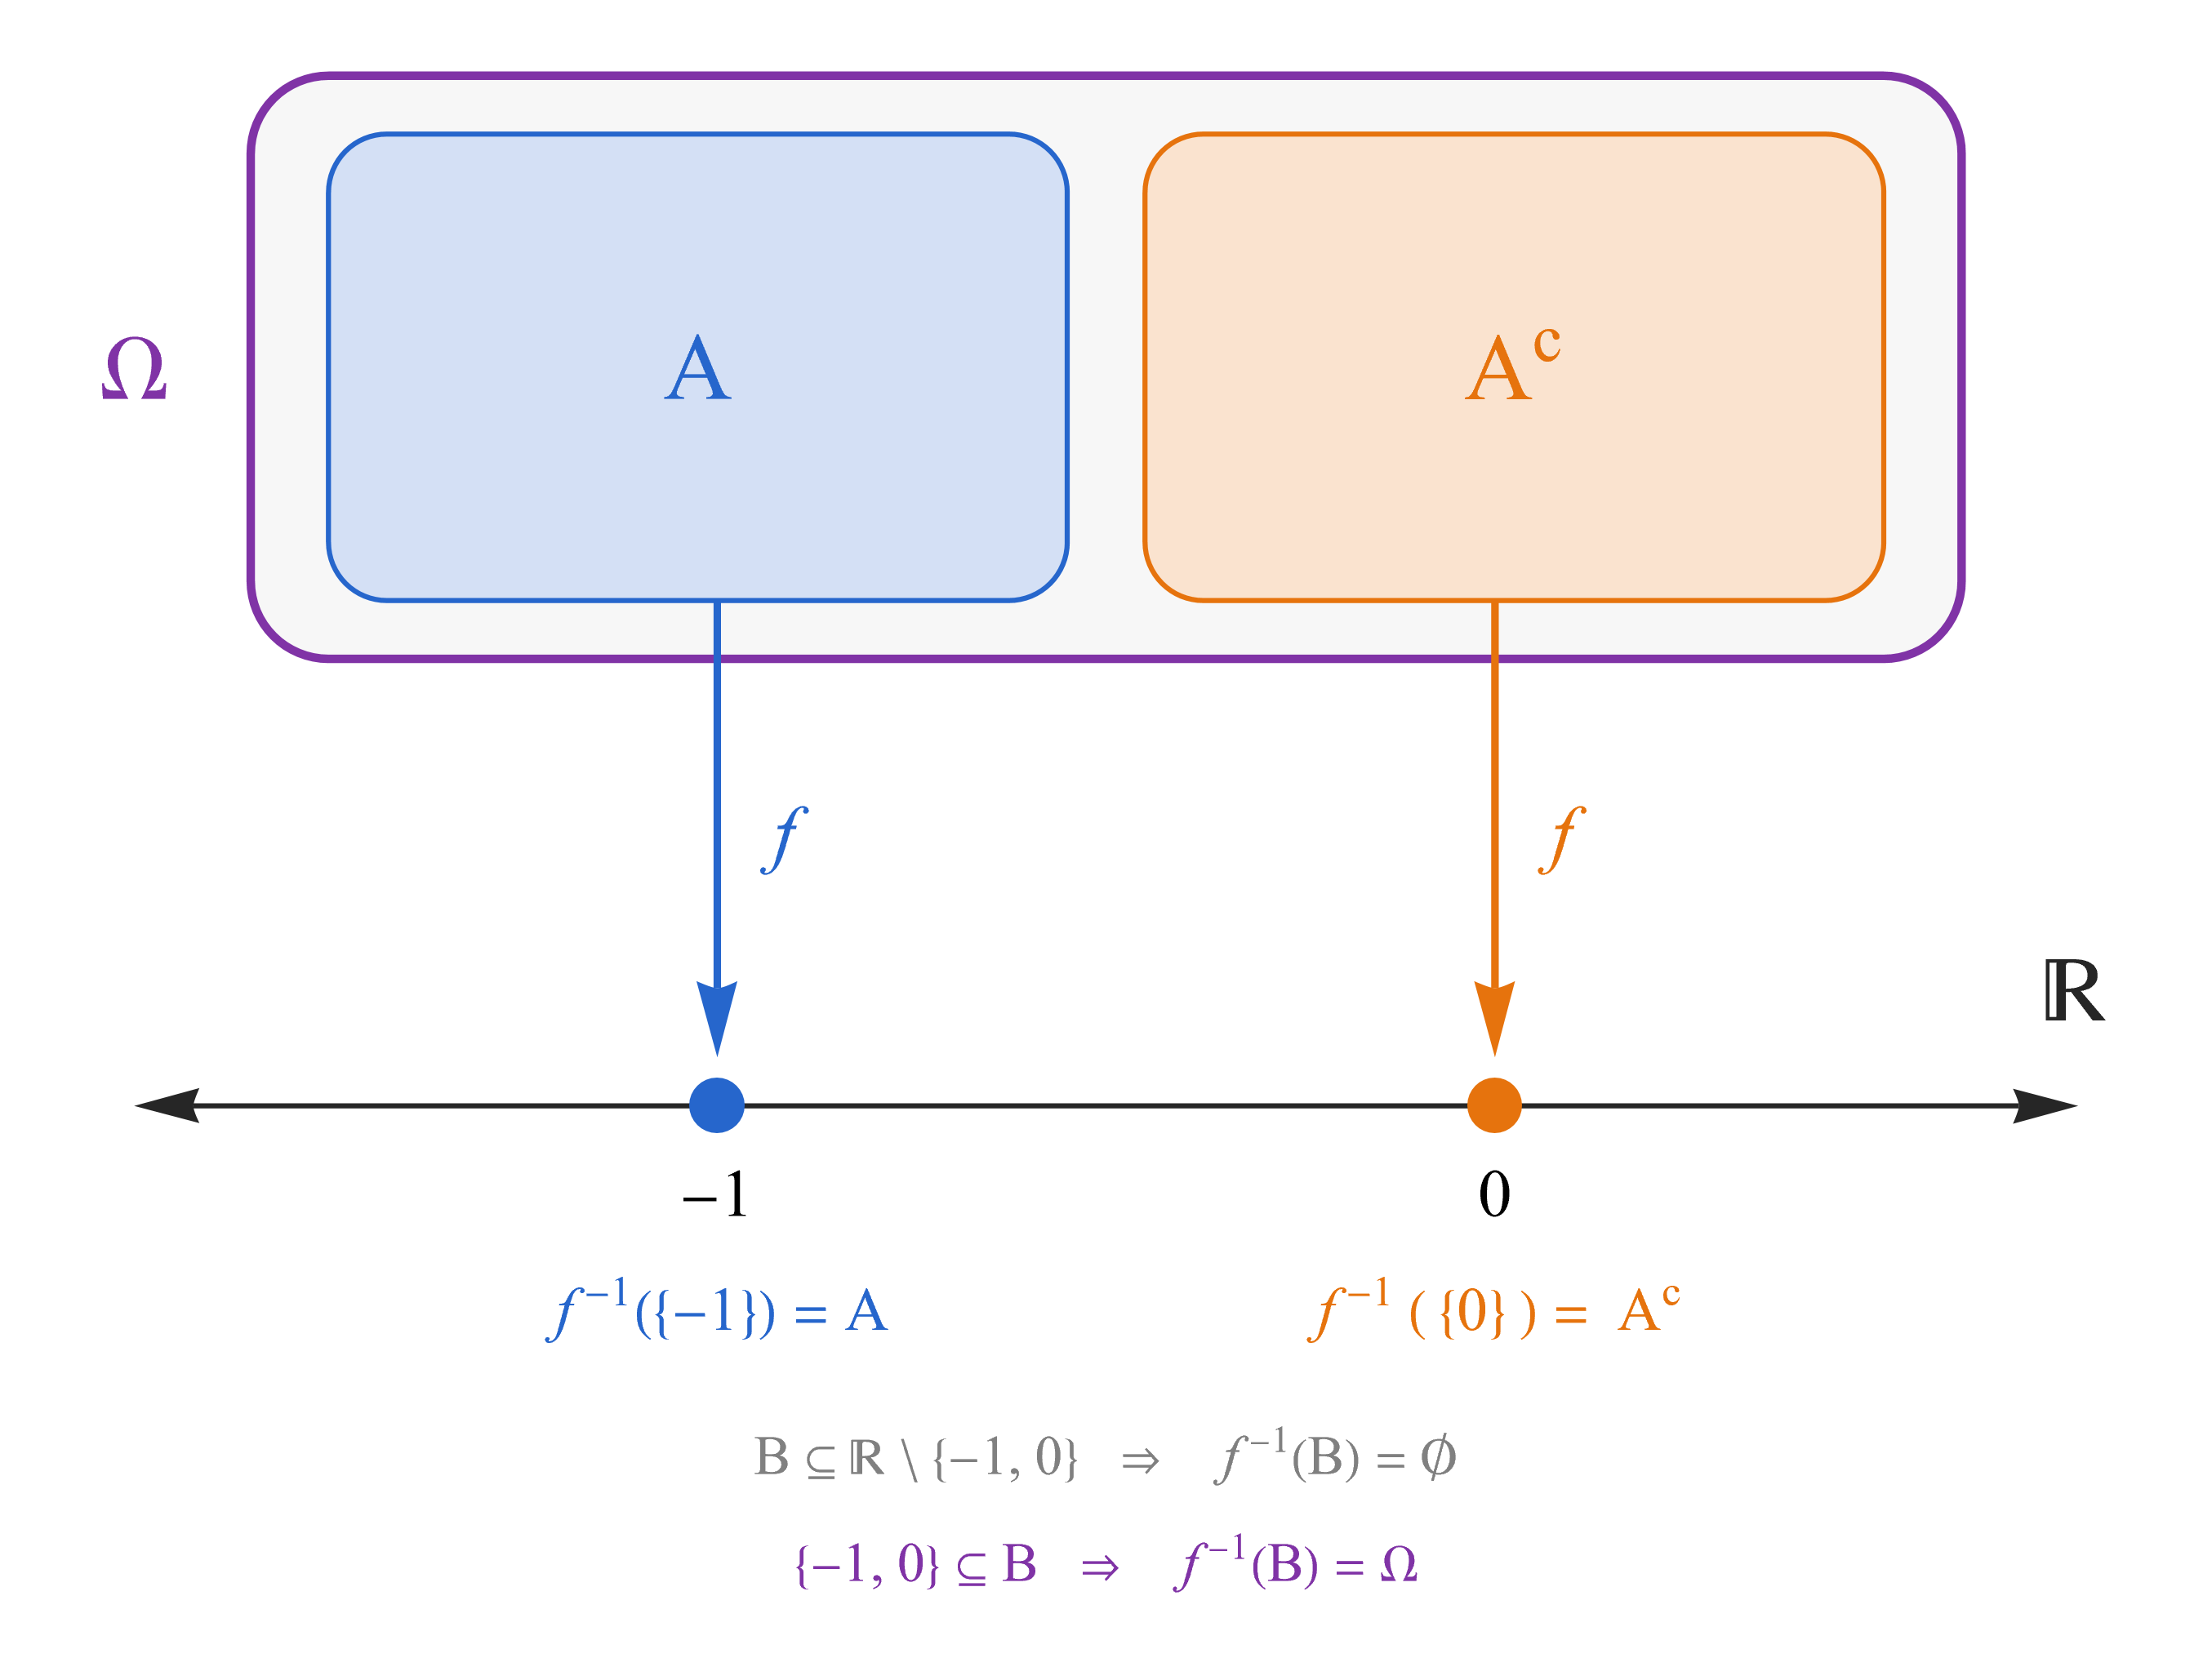
\includegraphics[width=0.95\linewidth]{imagenes/tema3/T3_P42_a.png}
\end{center}

\newpage
\textbf{Método 2: Comprobación mediante la clase generadora de semirrectas $(-\infty, x]$}

Por el Corolario de las clases generadoras, para probar la medibilidad de $f$ basta comprobar que la antiimagen de cualquier elemento de una clase que genere la $\sigma$-álgebra de Borel $\mathcal{B}$ pertenece a $\mathcal{G}$.

Consideramos la clase generadora $\mathcal{C} = \{(-\infty, x] \mid x \in \mathbb{R}\}$, tal que $\sigma(\mathcal{C}) = \mathcal{B}$. Evaluamos la antiimagen $f^{-1}((-\infty, x])$ según el valor de $x \in \mathbb{R}$:
\begin{itemize}
    \item Si $x < -1$: ningún valor de $\mathrm{Im}(f) = \{-1, 0\}$ está en $(-\infty, x]$, luego:
    \[
        f^{-1}((-\infty, x]) = \varnothing \in \mathcal{G}
    \]
    \item Si $-1 \le x < 0$: únicamente el valor $-1$ pertenece a $(-\infty, x]$, luego:
    \[
        f^{-1}((-\infty, x]) = A \in \mathcal{G}
    \]
    \item Si $x \ge 0$: ambos valores $\{-1, 0\}$ pertenecen a $(-\infty, x]$, luego:
    \[
        f^{-1}((-\infty, x]) = A \cup A^c = \Omega \in \mathcal{G}
    \]
\end{itemize}

Como $f^{-1}((-\infty, x]) \in \mathcal{G}$ para todo $x \in \mathbb{R}$, se concluye que $f$ es medible respecto a $(\mathcal{G}, \mathcal{B})$.

\begin{center}
    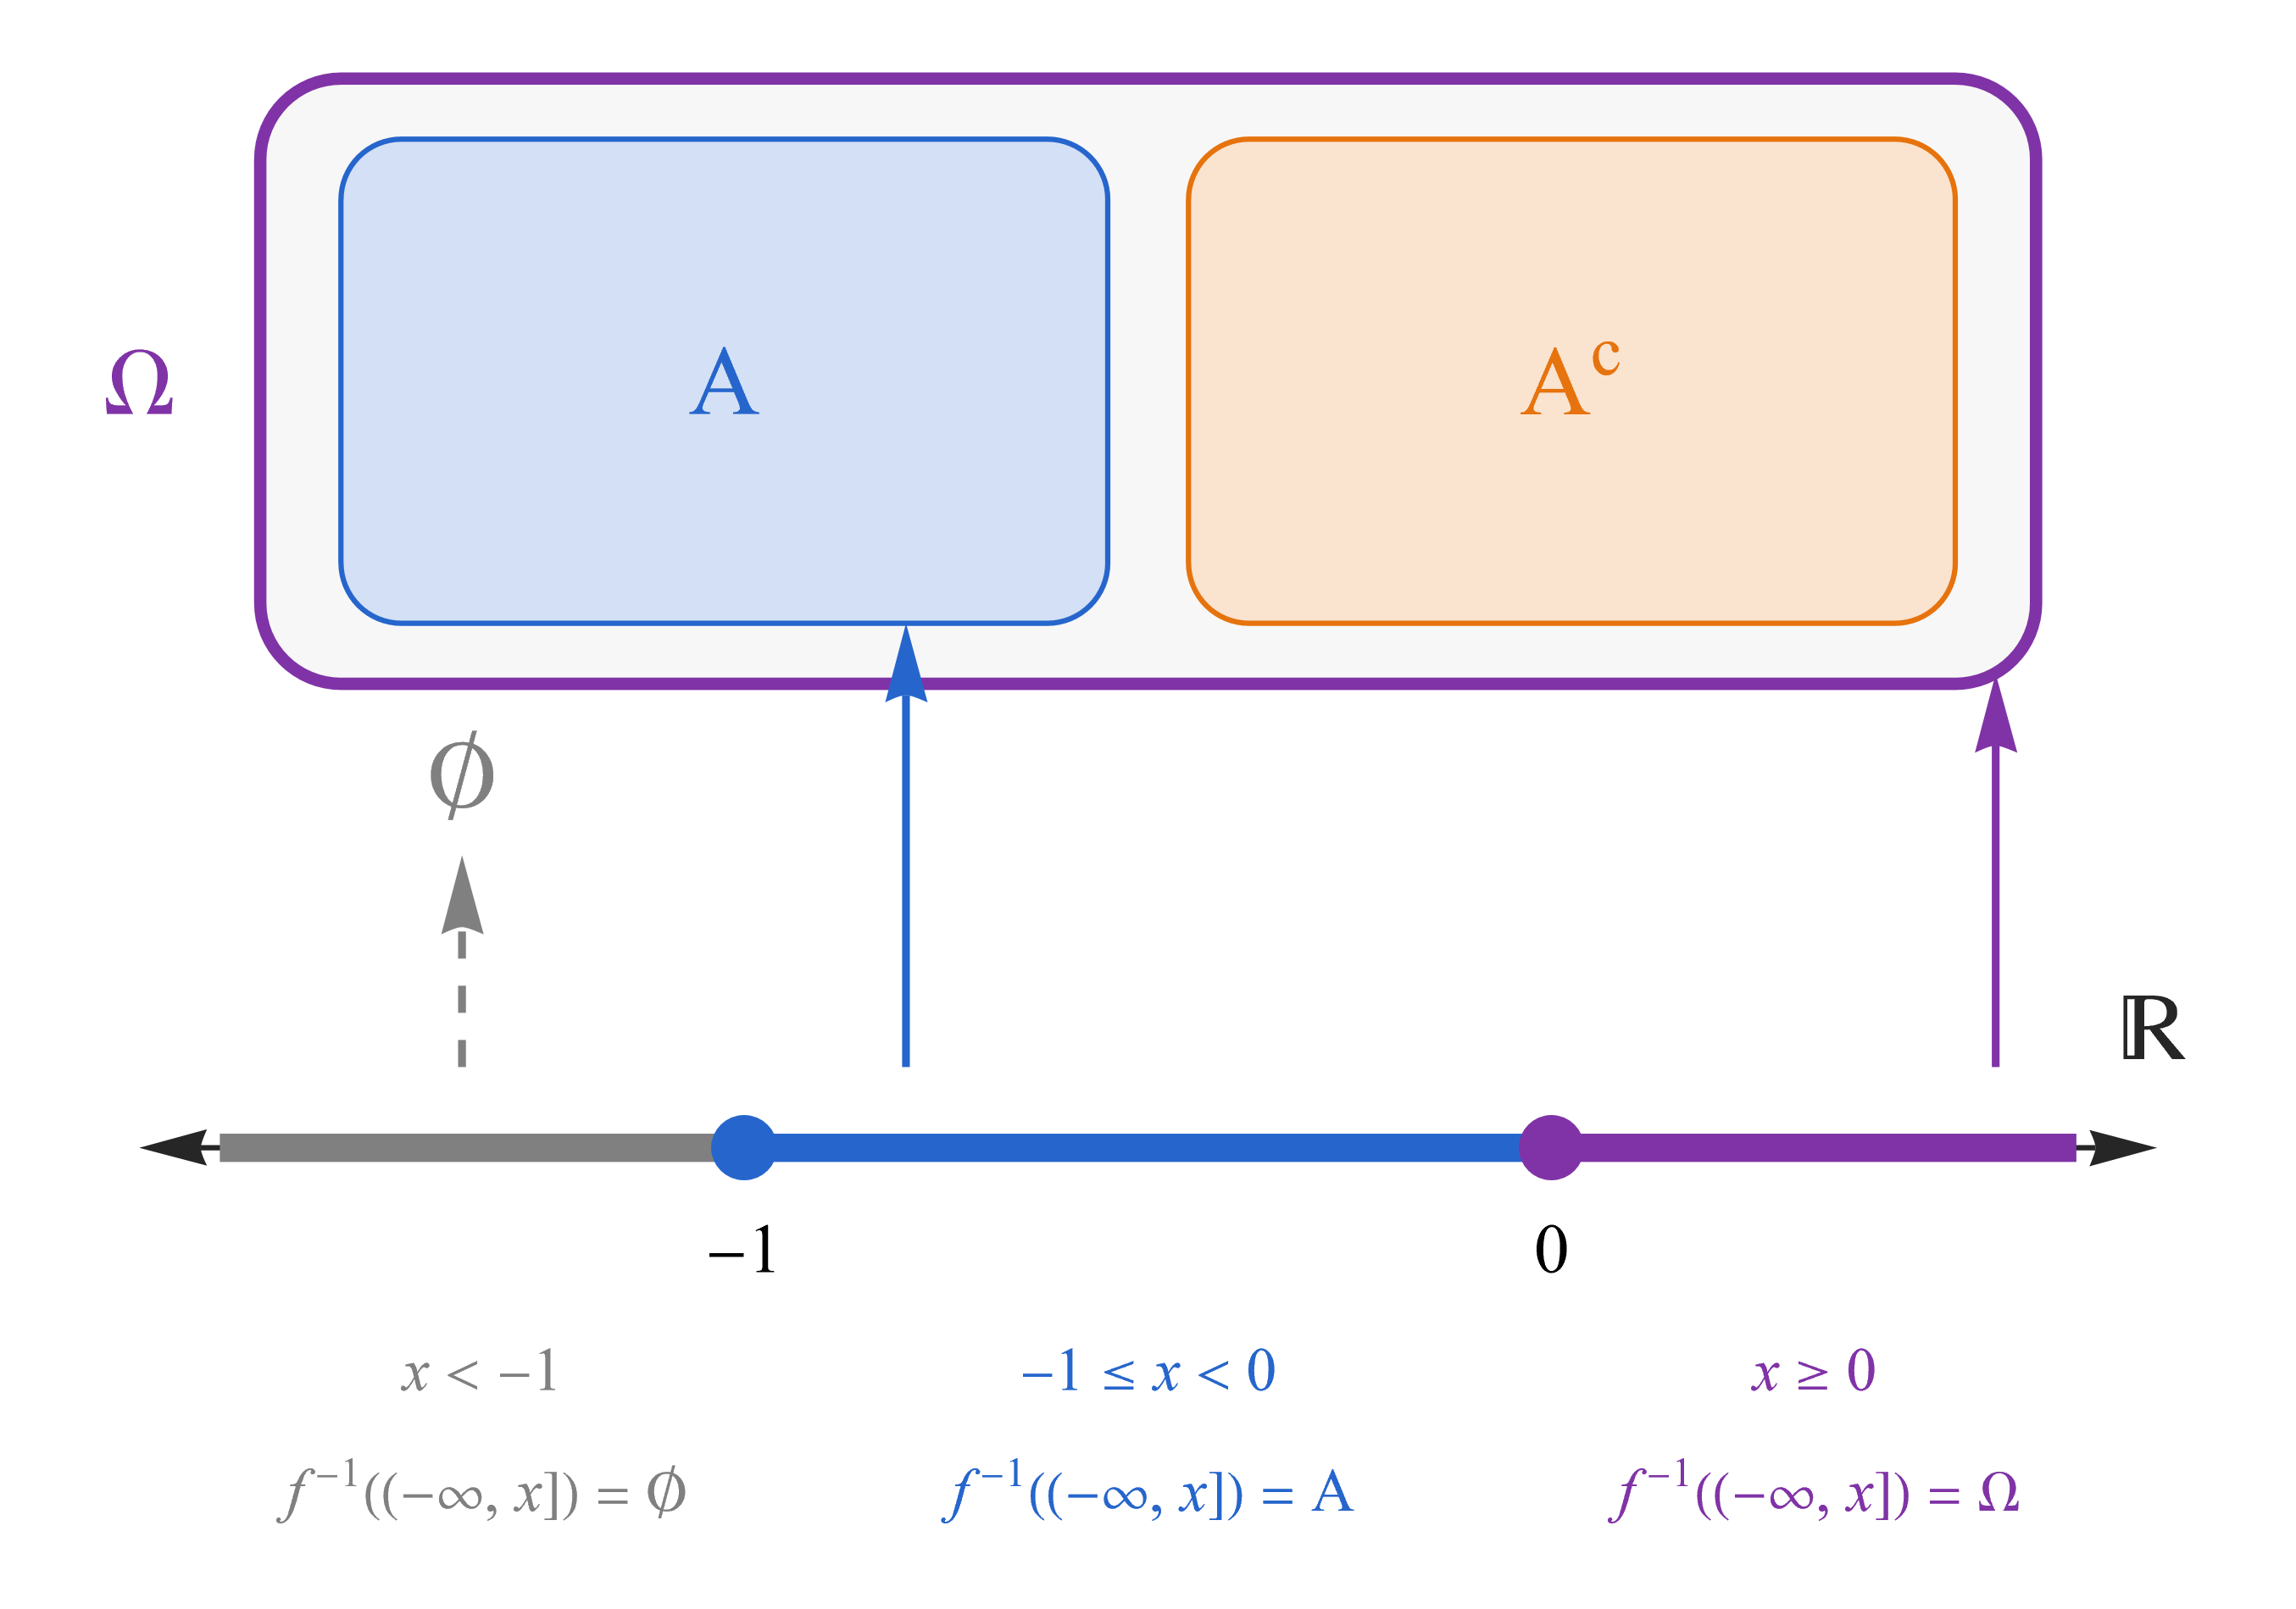
\includegraphics[width=0.95\linewidth]{imagenes/tema3/T3_P42_b.png}
\end{center}
\end{problema}

\textbf{Nota sobre funciones simples:} Alternativamente, $f$ se puede expresar como $f = -\mathbf{1}_A + 0 \cdot \mathbf{1}_{A^c} = -\mathbf{1}_A$. Al ser $A \in \mathcal{G}$ un conjunto medible, su función indicadora $\mathbf{1}_A$ es simple y medible, por lo que $f$ es trivialmente medible.
\newpage
%===================
% Problema 43: 
%===================
\begin{problema}[Medibilidad de la función parte entera bajo distintas $\sigma$-álgebras]
Sea $f : (\mathbb{R}^+, \mathcal{G}) \to (\mathbb{N}, \mathcal{H})$ la aplicación parte entera definida por $f(x) = \lfloor x \rfloor$, que asigna a cada número real no negativo su parte entera. Determinar si $f$ es medible en los siguientes casos:
\begin{enumerate}[label=\alph*)]
    \item $\mathcal{G} = \mathcal{B}^+$ (la $\sigma$-álgebra de Borel sobre $\mathbb{R}^+$) y $\mathcal{H} = \mathcal{P}(\mathbb{N})$.
    \item $\mathcal{G} = \mathcal{B}^+$ y $\mathcal{H} = \{\mathbb{N}, \varnothing, \{1,2,3\}, \mathbb{N} \setminus \{1,2,3\}\}$.
    \item $\mathcal{G} = \{\mathbb{R}^+, \varnothing, [0,10), [10,\infty)\}$ y $\mathcal{H} = \mathcal{P}(\mathbb{N})$.
\end{enumerate}

\tcblower

\textbf{a) Caso $\mathcal{G} = \mathcal{B}^+$ y $\mathcal{H} = \mathcal{P}(\mathbb{N})$:}

Para analizar la medibilidad de $f$, aplicamos el criterio de las clases generadoras. La $\sigma$-álgebra de partes $\mathcal{P}(\mathbb{N})$ está generada por la colección de subconjuntos unipuntuales $\mathcal{C} = \{\{n\} \mid n \in \mathbb{N}\}$, de modo que $\sigma(\mathcal{C}) = \mathcal{P}(\mathbb{N})$.

Calculamos la imagen inversa de un elemento genérico $\{n\} \in \mathcal{C}$:
\[
    f^{-1}(\{n\}) = \{x \in \mathbb{R}^+ \mid \lfloor x \rfloor = n\} = [n, n+1)
\]
Puesto que los intervalos semiabiertos $[n, n+1)$ son subconjuntos borelianos de $\mathbb{R}^+$, tenemos que $f^{-1}(\{n\}) \in \mathcal{B}^+$ para todo $n \in \mathbb{N}$.

Al cumplirse que $f^{-1}(\mathcal{C}) \subseteq \mathcal{B}^+$, se concluye que \textbf{$f$ es una función medible}.

\begin{center}
    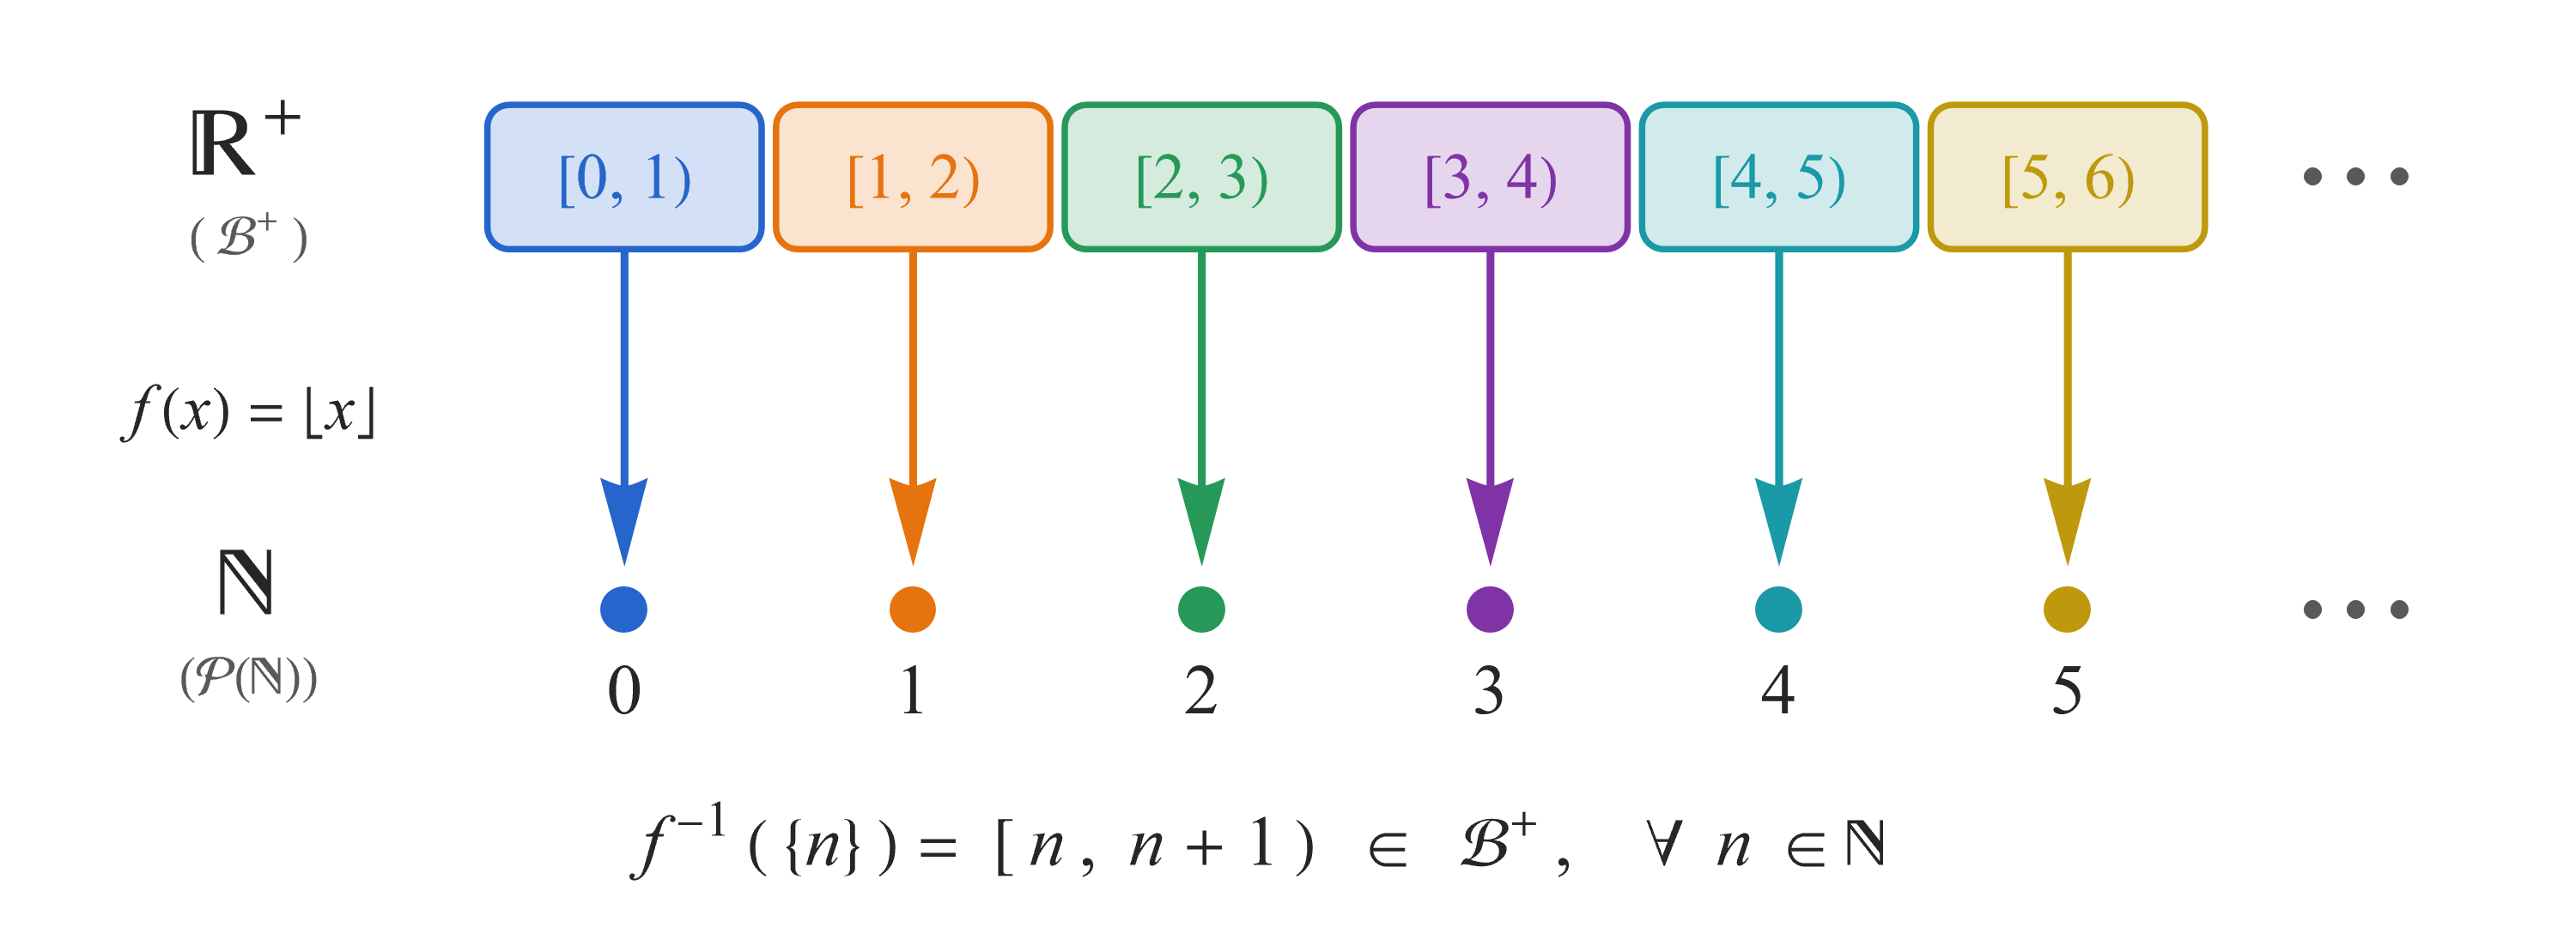
\includegraphics[width=0.95\linewidth]{imagenes/tema3/T3_P43_a.png}
\end{center}
\textbf{b) Caso $\mathcal{G} = \mathcal{B}^+$ y $\mathcal{H} = \{\mathbb{N}, \varnothing, \{1,2,3\}, \mathbb{N} \setminus \{1,2,3\}\}$:}

En este caso, $\mathcal{H}$ es una $\sigma$-álgebra finita. Para verificar la medibilidad de $f$, comprobamos que la antiimagen de cada uno de los elementos de $\mathcal{H}$ pertenece a la $\sigma$-álgebra de Borel $\mathcal{B}^+$:
\begin{itemize}
    \item $f^{-1}(\varnothing) = \varnothing \in \mathcal{B}^+$.
    \item $f^{-1}(\mathbb{N}) = \mathbb{R}^+ \in \mathcal{B}^+$.
    \item $f^{-1}(\{1,2,3\}) = [1, 2) \cup [2, 3) \cup [3, 4) = [1, 4) \in \mathcal{B}^+$.
    \item $f^{-1}(\mathbb{N} \setminus \{1,2,3\}) = (f^{-1}(\{1,2,3\}))^c = \mathbb{R}^+ \setminus [1, 4) = [0, 1) \cup [4, \infty) \in \mathcal{B}^+$.
\end{itemize}

Dado que la antiimagen de cualquier suceso de $\mathcal{H}$ es un conjunto boreliano en $\mathbb{R}^+$, concluimos que \textbf{$f$ es una función medible}.

\begin{center}
    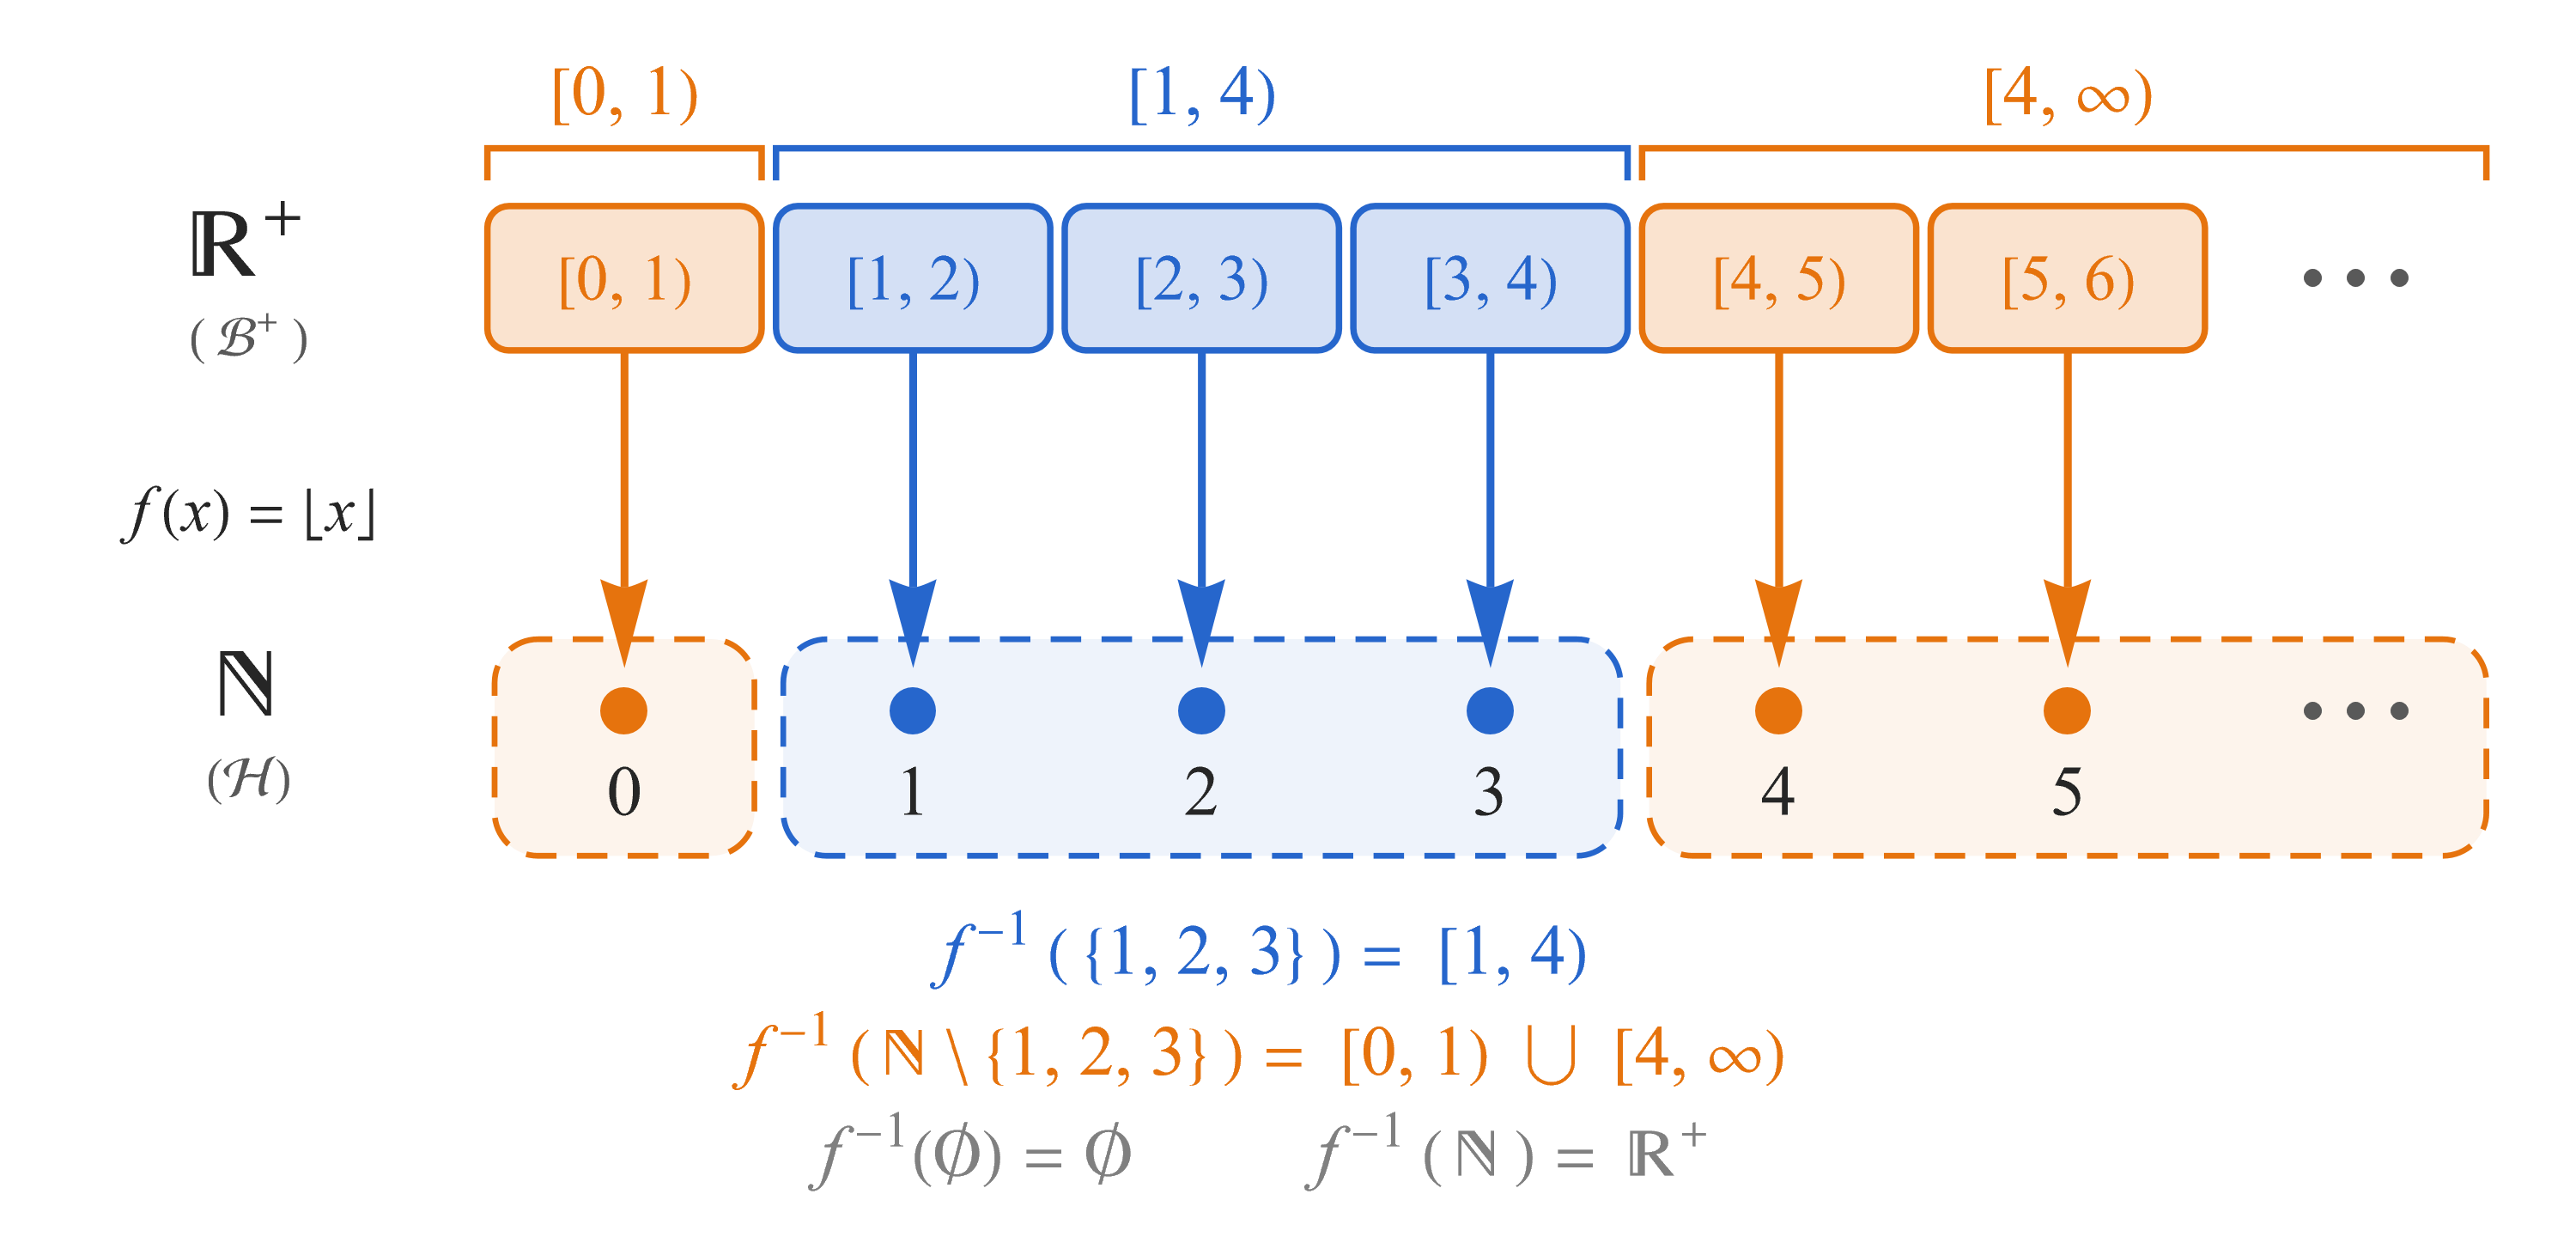
\includegraphics[width=0.95\linewidth]{imagenes/tema3/T3_P43_b.png}
\end{center}

\textbf{c) Caso $\mathcal{G} = \{\mathbb{R}^+, \varnothing, [0,10), [10,\infty)\}$ y $\mathcal{H} = \mathcal{P}(\mathbb{N})$:}

La $\sigma$-álgebra de llegada $\mathcal{H} = \mathcal{P}(\mathbb{N})$ contiene todos los subconjuntos de $\mathbb{N}$, mientras que la $\sigma$-álgebra de partida $\mathcal{G}$ es muy restringida y solo consta de cuatro elementos: $\mathcal{G} = \{\varnothing, \mathbb{R}^+, [0,10), [10,\infty)\}$.

Para demostrar que $f$ no es medible, basta encontrar un suceso de $\mathcal{H}$ cuya antiimagen no pertenezca a $\mathcal{G}$.

Tomemos, por ejemplo, el conjunto unipuntual $\{1\} \in \mathcal{P}(\mathbb{N})$. Su antiimagen por la función parte entera es:
\[
    f^{-1}(\{1\}) = \{x \in \mathbb{R}^+ \mid \lfloor x \rfloor = 1\} = [1, 2)
\]
Sin embargo, el intervalo $[1, 2) \notin \mathcal{G}$, puesto que los únicos subconjuntos no triviales de $\mathcal{G}$ son $[0,10)$ y $[10,\infty)$.

Por consiguiente, $f^{-1}(\mathcal{H}) \not\subseteq \mathcal{G}$, lo que demuestra formalmente que \textbf{$f$ no es una función medible} en este caso.
\begin{center}
    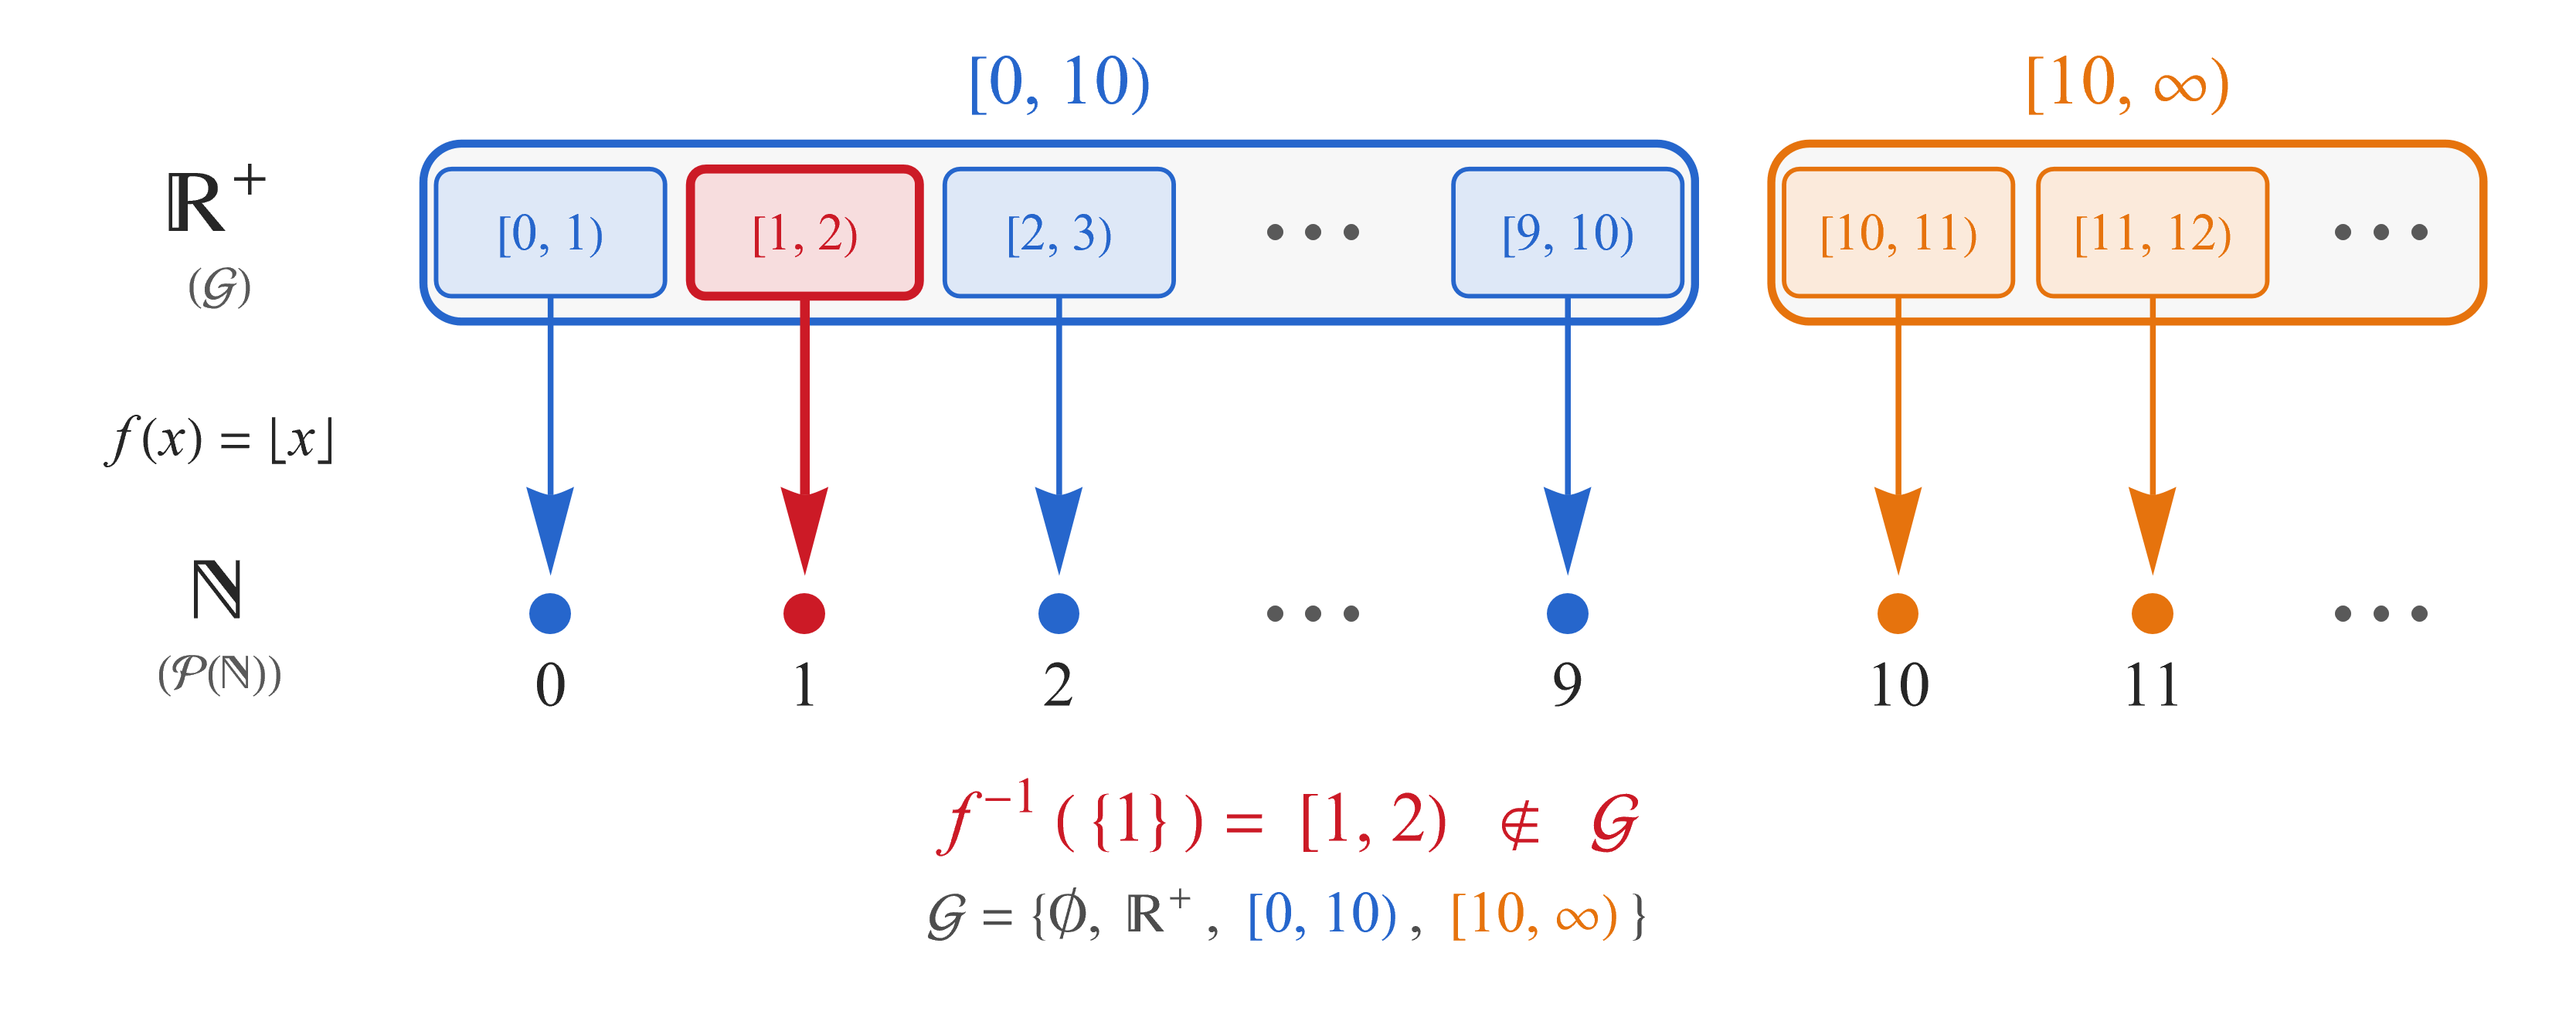
\includegraphics[width=0.95\linewidth]{imagenes/tema3/T3_P43_c.png}
\end{center}
\end{problema}

\newpage
%===================
% Problema 44: 
%===================
\begin{problema}[Medibilidad de una función definida a trozos sobre un conjunto medible]
Sean $f, g : (\Omega, \mathcal{G}) \to (\Omega', \mathcal{G}')$ dos aplicaciones medibles entre los espacios medibles $(\Omega, \mathcal{G})$ y $(\Omega', \mathcal{G}')$. Sea $A \in \mathcal{G}$ un suceso medible del espacio de partida. Se define la función $h : \Omega \to \Omega'$ por:
\[
    h(\omega) = \begin{cases} f(\omega) & \text{si } \omega \in A \\ g(\omega) & \text{si } \omega \notin A \end{cases}
\]
Demostrar que $h : (\Omega, \mathcal{G}) \to (\Omega', \mathcal{G}')$ es una aplicación medible.

\tcblower

Para demostrar la medibilidad de la aplicación $h$, debemos probar que la imagen inversa de cualquier suceso medible $B \in \mathcal{G}'$ del espacio de llegada pertenece a la $\sigma$-álgebra $\mathcal{G}$ del espacio de partida, es decir, $h^{-1}(B) \in \mathcal{G}$ para todo $B \in \mathcal{G}'$.

\paragraph{1. Descomposición de la antiimagen:}
Sea $B \in \mathcal{G}'$ un subconjunto medible arbitrario. Expresamos el espacio de partida $\Omega$ como la unión disjunta del conjunto $A$ y su complementario $A^c$ ($\Omega = A \cup A^c$). Utilizando las propiedades de la imagen inversa y distribuyendo respecto a esta partición:
\[
    h^{-1}(B) = h^{-1}(B) \cap \Omega = h^{-1}(B) \cap (A \cup A^c) = (h^{-1}(B) \cap A) \cup (h^{-1}(B) \cap A^c)
\]

\paragraph{2. Restricción de $h$ sobre los bloques de la partición:}
Analizamos el comportamiento de la función $h$ en cada subdominio:
\begin{itemize}
    \item Para todo $\omega \in A$, la función coincide con $f(\omega)$, por lo que:
    \[
        h^{-1}(B) \cap A = \{\omega \in A \mid h(\omega) \in B\} = \{\omega \in A \mid f(\omega) \in B\} = f^{-1}(B) \cap A
    \]
    \item Para todo $\omega \in A^c$, la función coincide con $g(\omega)$, por lo que:
    \[
        h^{-1}(B) \cap A^c = \{\omega \in A^c \mid h(\omega) \in B\} = \{\omega \in A^c \mid g(\omega) \in B\} = g^{-1}(B) \cap A^c
    \]
\end{itemize}

Sustituyendo ambas identidades en la descomposición de $h^{-1}(B)$, obtenemos la representación fundamental:
\[
    h^{-1}(B) = (f^{-1}(B) \cap A) \cup (g^{-1}(B) \cap A^c)
\]

\begin{center}
    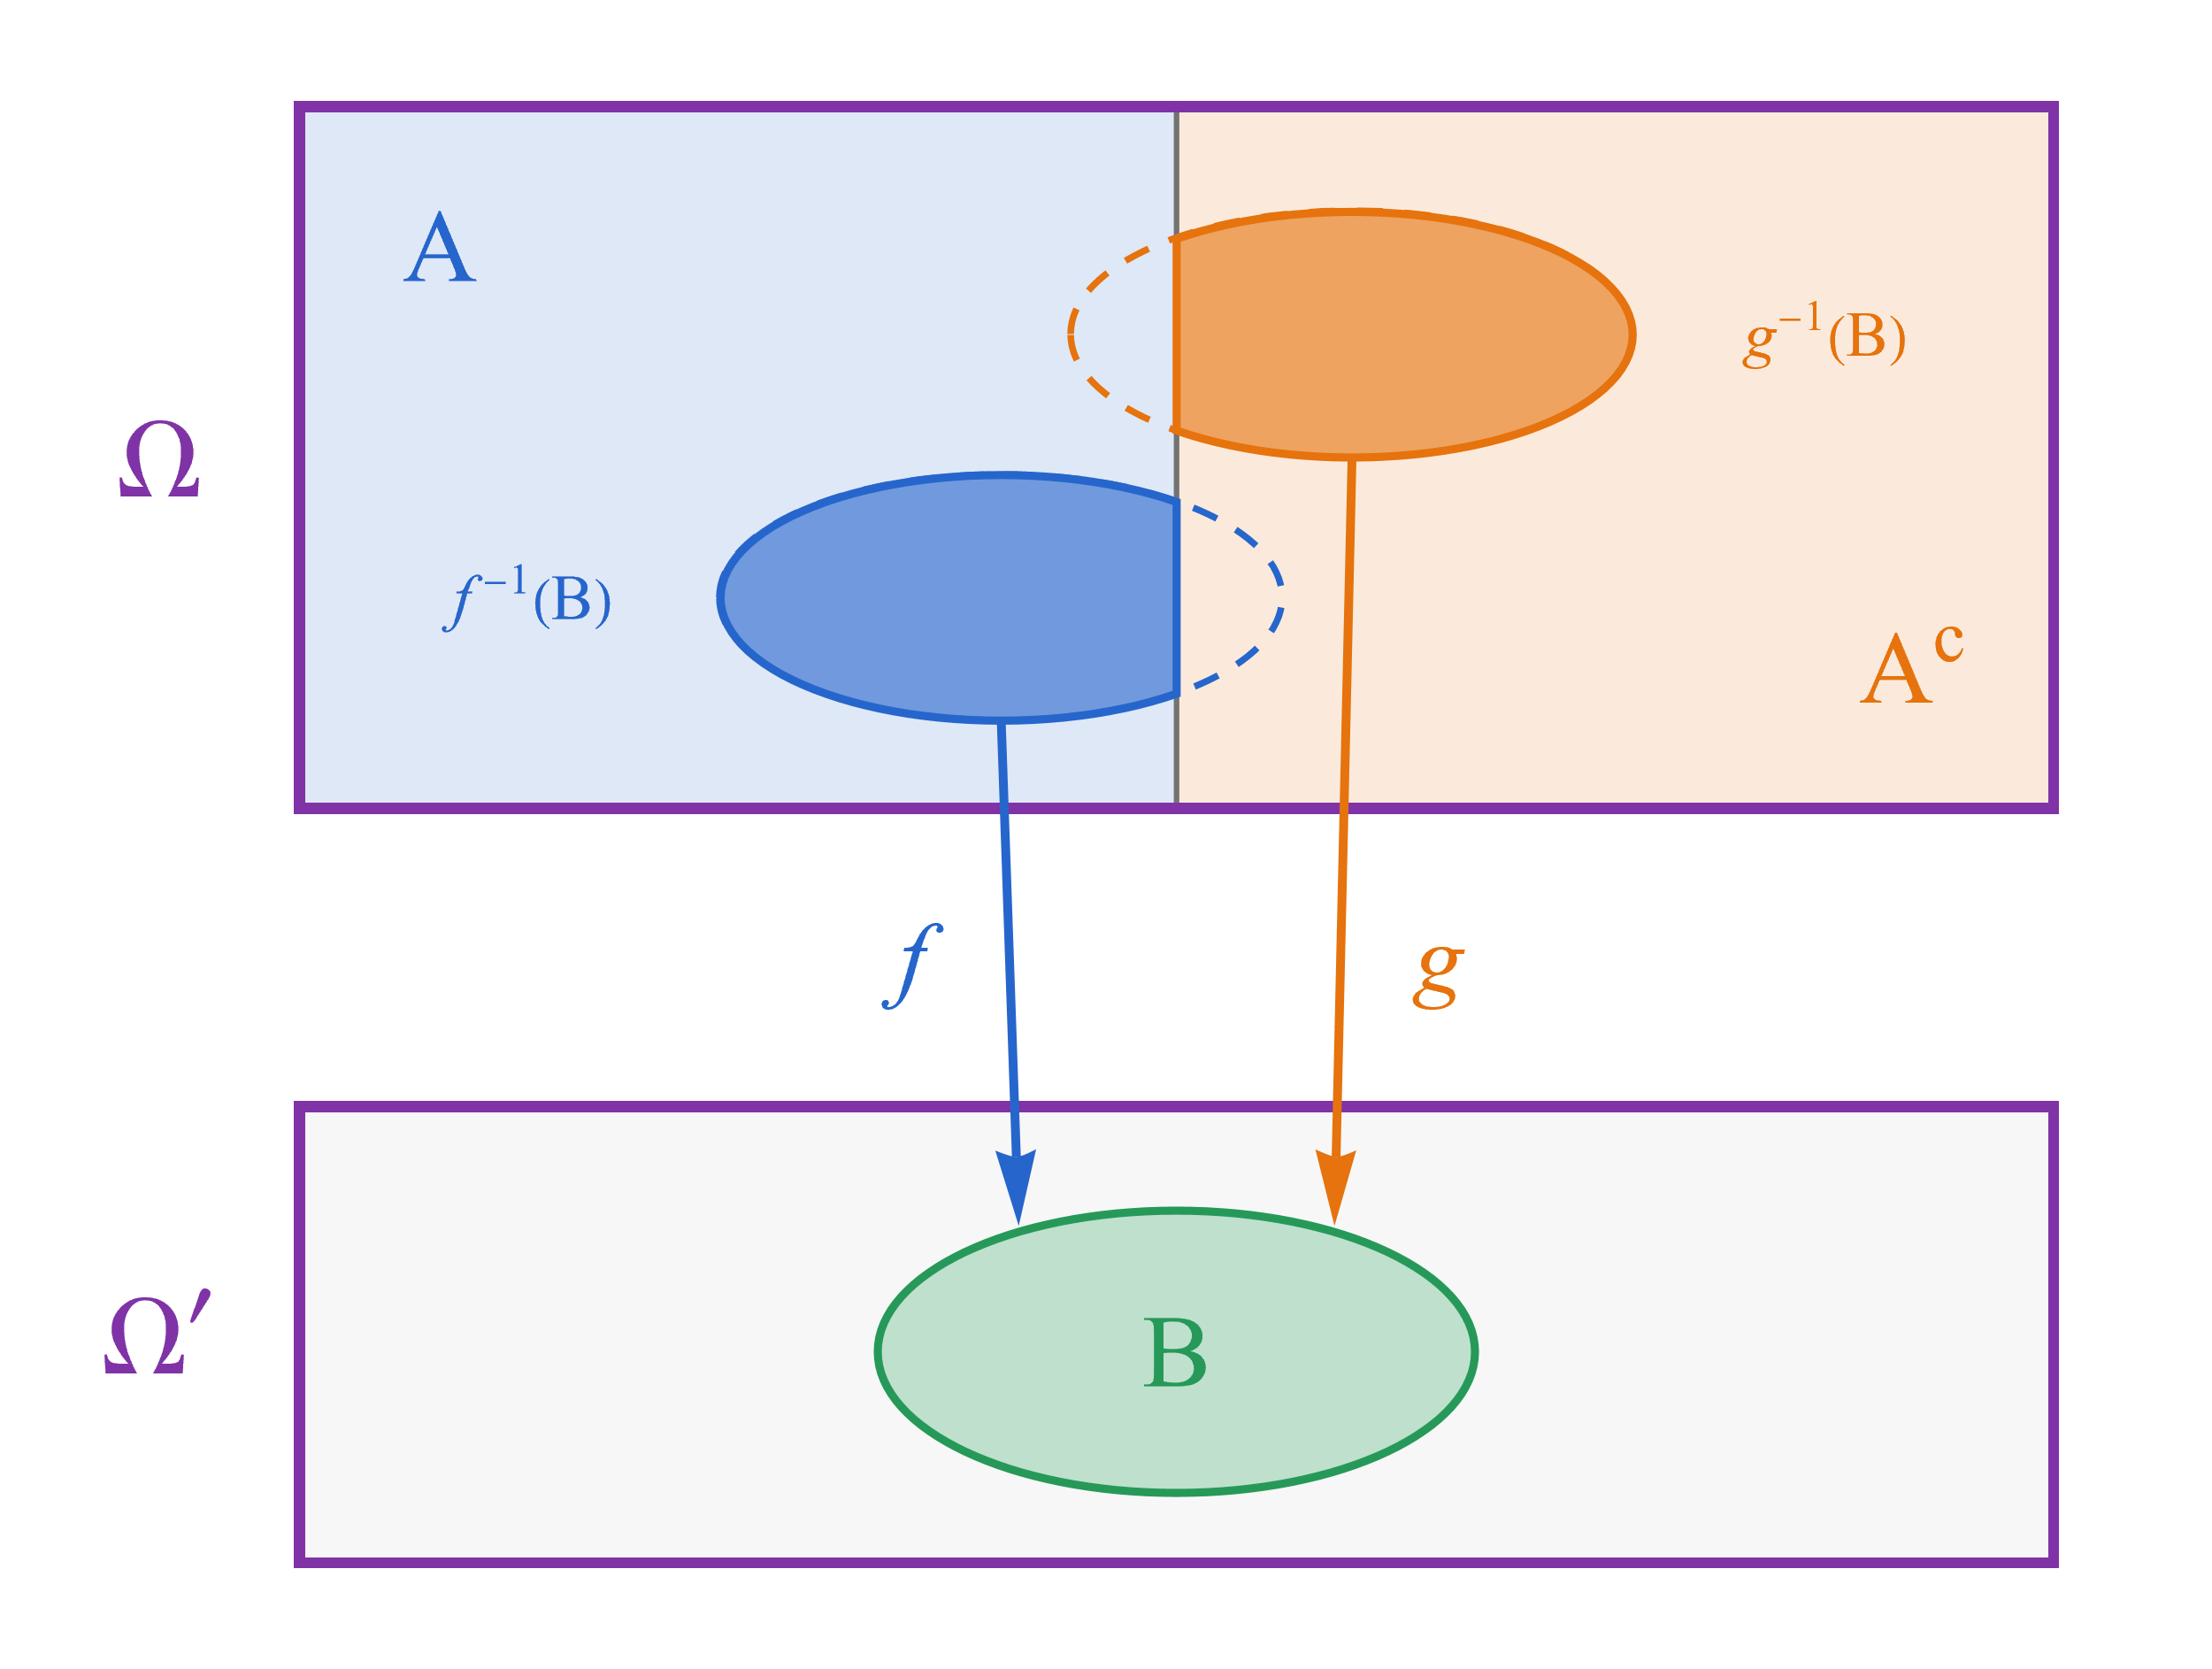
\includegraphics[width=0.75\linewidth]{imagenes/tema3/T3_P44_a.png}
\end{center}

\paragraph{3. Comprobación de la pertenencia a la $\sigma$-álgebra $\mathcal{G}$:}
Analizamos la medibilidad de cada uno de los componentes de la unión:
\begin{enumerate}[label=\arabic*.]
    \item Puesto que $f : (\Omega, \mathcal{G}) \to (\Omega', \mathcal{G}')$ es una aplicación medible, por definición $f^{-1}(B) \in \mathcal{G}$.
    \item Puesto que $g : (\Omega, \mathcal{G}) \to (\Omega', \mathcal{G}')$ es una aplicación medible, por definición $g^{-1}(B) \in \mathcal{G}$.
    \item Por hipótesis $A \in \mathcal{G}$, y al ser $\mathcal{G}$ una $\sigma$-álgebra, es cerrada bajo complementación, luego $A^c \in \mathcal{G}$.
    \item Dado que las $\sigma$-álgebras son cerradas bajo intersecciones finitas:
    \[
        f^{-1}(B) \cap A \in \mathcal{G} \quad \text{y} \quad g^{-1}(B) \cap A^c \in \mathcal{G}
    \]
    \item Por último, la estabilidad bajo uniones finitas garantiza que:
    \[
        h^{-1}(B) = (f^{-1}(B) \cap A) \cup (g^{-1}(B) \cap A^c) \in \mathcal{G}
    \]
\end{enumerate}

Por lo tanto, la imagen inversa $h^{-1}(B)$ pertenece a $\mathcal{G}$ para todo $B \in \mathcal{G}'$, lo que demuestra que $h$ es una aplicación medible.
\end{problema}

\newpage
%===================
% Problema 45: 
%===================
\begin{problema}[Medibilidad de aplicaciones coincidentes casi seguro en un espacio completo]
Sea $(\Omega, \mathcal{G}, \mu)$ un espacio de medida completo. Sean $f, g : (\Omega, \mathcal{G}) \to (\Omega', \mathcal{G}')$ dos aplicaciones entre los espacios medibles $(\Omega, \mathcal{G})$ y $(\Omega', \mathcal{G}')$, donde $f$ es una aplicación medible y $g \equiv f$ salvo en un subconjunto $A \in \mathcal{G}$ de medida nula ($\mu(A) = 0$), es decir, $g(\omega) = f(\omega)$ para todo $\omega \in A^c$. Demostrar que $g$ es una aplicación medible.

\tcblower

Para demostrar que $g : (\Omega, \mathcal{G}) \to (\Omega', \mathcal{G}')$ es una aplicación medible, debemos probar que para cualquier suceso medible $B \in \mathcal{G}'$ del espacio de llegada, su antiimagen $g^{-1}(B)$ pertenece a la $\sigma$-álgebra $\mathcal{G}$ del espacio de partida.

\paragraph{1. Descomposición de la antiimagen:}
Sea $B \in \mathcal{G}'$ un suceso arbitrario. Considerando la partición del espacio muestral $\Omega = A^c \cup A$, expresamos la antiimagen $g^{-1}(B)$ como la unión disjunta:
\[
    g^{-1}(B) = (g^{-1}(B) \cap A^c) \cup (g^{-1}(B) \cap A)
\]

\paragraph{2. Análisis sobre el complementario $A^c$:}
Por hipótesis, la aplicación $g$ coincide con $f$ sobre $A^c$ ($g(\omega) = f(\omega), \, \forall \omega \in A^c$). En consecuencia:
\[
    g^{-1}(B) \cap A^c = f^{-1}(B) \cap A^c
\]
Analizamos la pertenencia a $\mathcal{G}$ de esta intersección:
\begin{itemize}
    \item Puesto que $f$ es una aplicación medible, por definición $f^{-1}(B) \in \mathcal{G}$.
    \item Como $A \in \mathcal{G}$ y $\mathcal{G}$ es una $\sigma$-álgebra, el complementario $A^c \in \mathcal{G}$.
    \item La estabilidad de $\mathcal{G}$ respecto a intersecciones finitas garantiza que $f^{-1}(B) \cap A^c \in \mathcal{G}$.
\end{itemize}

\paragraph{3. Análisis sobre el conjunto de medida nula $A$:}
Consideramos ahora el segundo término de la unión, $g^{-1}(B) \cap A$:
\begin{itemize}
    \item Por construcción, este conjunto es un subconjunto de $A$:
    \[
        (g^{-1}(B) \cap A) \subseteq A
    \]
    \item Dado que $(\Omega, \mathcal{G}, \mu)$ es un \textbf{espacio de medida completo} y $A \in \mathcal{G}$ satisface $\mu(A) = 0$, todo subconjunto de $A$ es automáticamente medible y pertenece a $\mathcal{G}$ (con medida nula).
    \item Por tanto, $g^{-1}(B) \cap A \in \mathcal{G}$.
\end{itemize}

\begin{center}
    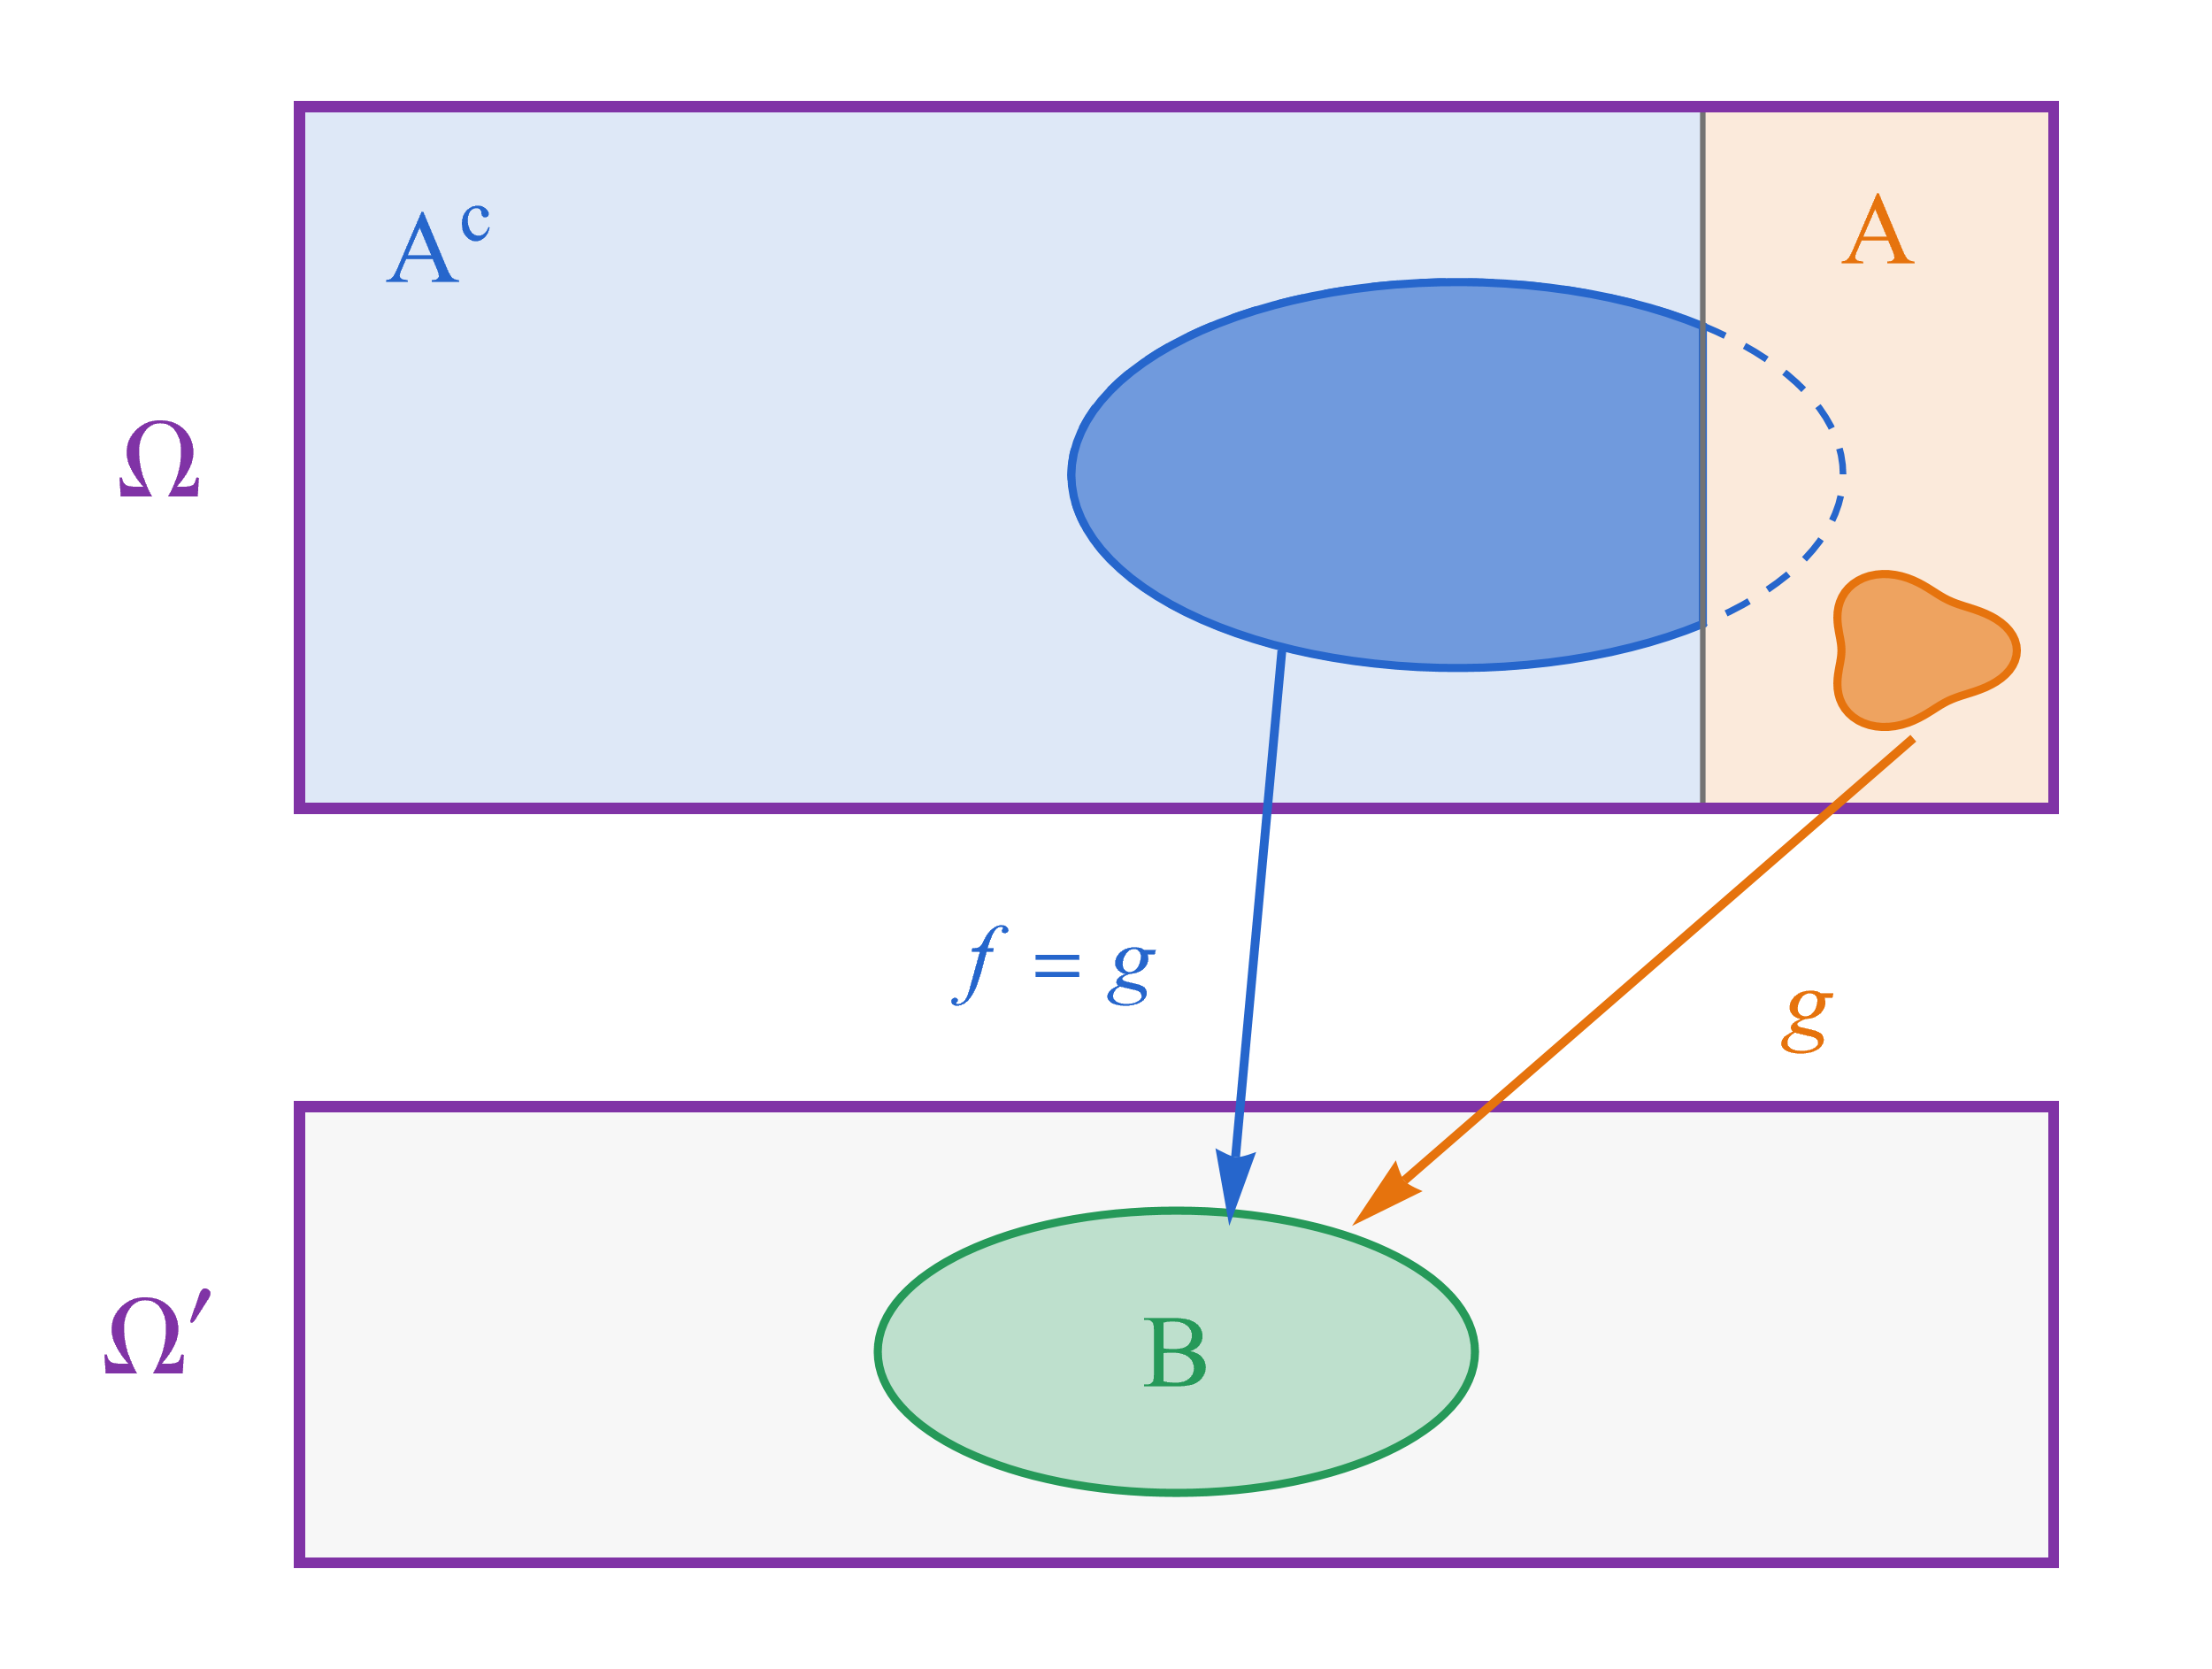
\includegraphics[width=0.95\linewidth]{imagenes/tema3/T3_P45_a.png}
\end{center}

\paragraph{4. Conclusión:}
Al ser la $\sigma$-álgebra $\mathcal{G}$ cerrada bajo uniones finitas, expresamos $g^{-1}(B)$ como unión de dos elementos de $\mathcal{G}$:
\[
    g^{-1}(B) = (f^{-1}(B) \cap A^c) \cup (g^{-1}(B) \cap A) \in \mathcal{G}
\]
Por lo tanto, la antiimagen de cualquier suceso $B \in \mathcal{G}'$ por $g$ es un conjunto medible, lo que demuestra formalmente que $g$ es una aplicación medible.
\end{problema}

\newpage
%===================
% Problema 46: 
%===================
\begin{problema}[Estudio de medibilidad mediante la antiimagen de distintas clases generadoras]
Estudiar si es medible la función $f : (\mathbb{R}, \mathcal{B}) \to (\mathbb{R}, \mathcal{B})$ definida por:
\[
    f(\omega) = \begin{cases} \omega & \text{si } \omega \le t \\ 1 & \text{si } \omega > t \end{cases} \qquad (\text{con } t < 1)
\]
utilizando como clases generadoras de la $\sigma$-álgebra de Borel $\mathcal{B}$:
\begin{enumerate}[label=\alph*)]
    \item Los intervalos de la forma $(a, b]$ con $a < b$.
    \item Los intervalos de la forma $(-\infty, x]$ con $x \in \mathbb{R}$.
\end{enumerate}

\tcblower

La medibilidad de la función $f : (\mathbb{R}, \mathcal{B}) \to (\mathbb{R}, \mathcal{B})$ se reduce a comprobar que la antiimagen de cualquier elemento de una clase generadora de $\mathcal{B}$ es un suceso boreliano (es decir, pertenece a $\mathcal{B}$).

Observamos que la imagen directa de $f$ es el conjunto $\mathrm{Im}(f) = (-\infty, t] \cup \{1\}$. Dado que $t < 1$, existe un intervalo de discontinuidad en la imagen dada por $(t, 1)$.

\textbf{a) Análisis con la clase generadora $\mathcal{C}_1 = \{(a, b] \mid a < b, \, a,b \in \mathbb{R}\}$:}

Calculamos la imagen inversa $f^{-1}((a, b])$ distinguiendo los casos según la posición de $a$ y $b$ respecto a $t$ y $1$:

\begin{itemize}
    \item \textbf{Caso 1 ($a < b \le t$):}
    Para $\omega \le t$, $f(\omega) = \omega \in (a, b] \iff \omega \in (a, b]$.
    Para $\omega > t$, $f(\omega) = 1 > t \ge b$, por lo que $1 \notin (a, b]$.
    \[
        f^{-1}((a, b]) = (a, b] \in \mathcal{B}
    \]

    \item \textbf{Caso 2 ($a < t < b < 1$):}
    Para $\omega \le t$, $f(\omega) = \omega \in (a, b] \iff \omega \in (a, t]$.
    Para $\omega > t$, $f(\omega) = 1 \notin (a, b]$ pues $b < 1$.
    \[
        f^{-1}((a, b]) = (a, t] \in \mathcal{B}
    \]

    \item \textbf{Caso 3 ($a < t$ y $b \ge 1$):}
    Para $\omega \le t$, $f(\omega) = \omega \in (a, b] \iff \omega \in (a, t]$.
    Para $\omega > t$, $f(\omega) = 1 \in (a, b]$ pues $a < t < 1 \le b$.
    \[
        f^{-1}((a, b]) = (a, t] \cup (t, \infty) = (a, \infty) \in \mathcal{B}
    \]

    \item \textbf{Caso 4 ($t \le a < 1$ y $b < 1$):}
    Para $\omega \le t$, $f(\omega) = \omega \le t \le a$, luego $f(\omega) \notin (a, b]$.
    Para $\omega > t$, $f(\omega) = 1 > b$, luego $f(\omega) \notin (a, b]$.
    \[
        f^{-1}((a, b]) = \varnothing \in \mathcal{B}
    \]

    \item \textbf{Caso 5 ($t \le a < 1$ y $b \ge 1$):}
    Para $\omega \le t$, $f(\omega) = \omega \le t \le a$, luego $f(\omega) \notin (a, b]$.
    Para $\omega > t$, $f(\omega) = 1 \in (a, b]$ pues $a < 1 \le b$.
    \[
        f^{-1}((a, b]) = (t, \infty) \in \mathcal{B}
    \]

    \item \textbf{Caso 6 ($a \ge 1$):}
    Para $\omega \le t$, $f(\omega) = \omega \le t < 1 \le a$.
    Para $\omega > t$, $f(\omega) = 1 \notin (a, b]$ pues $a \ge 1$.
    \[
        f^{-1}((a, b]) = \varnothing \in \mathcal{B}
    \]
\end{itemize}

En todos los casos posibles, $f^{-1}((a, b]) \in \mathcal{B}$. Por el Corolario de las clases generadoras, concluimos que \textbf{$f$ es una función medible}.

\begin{center}
    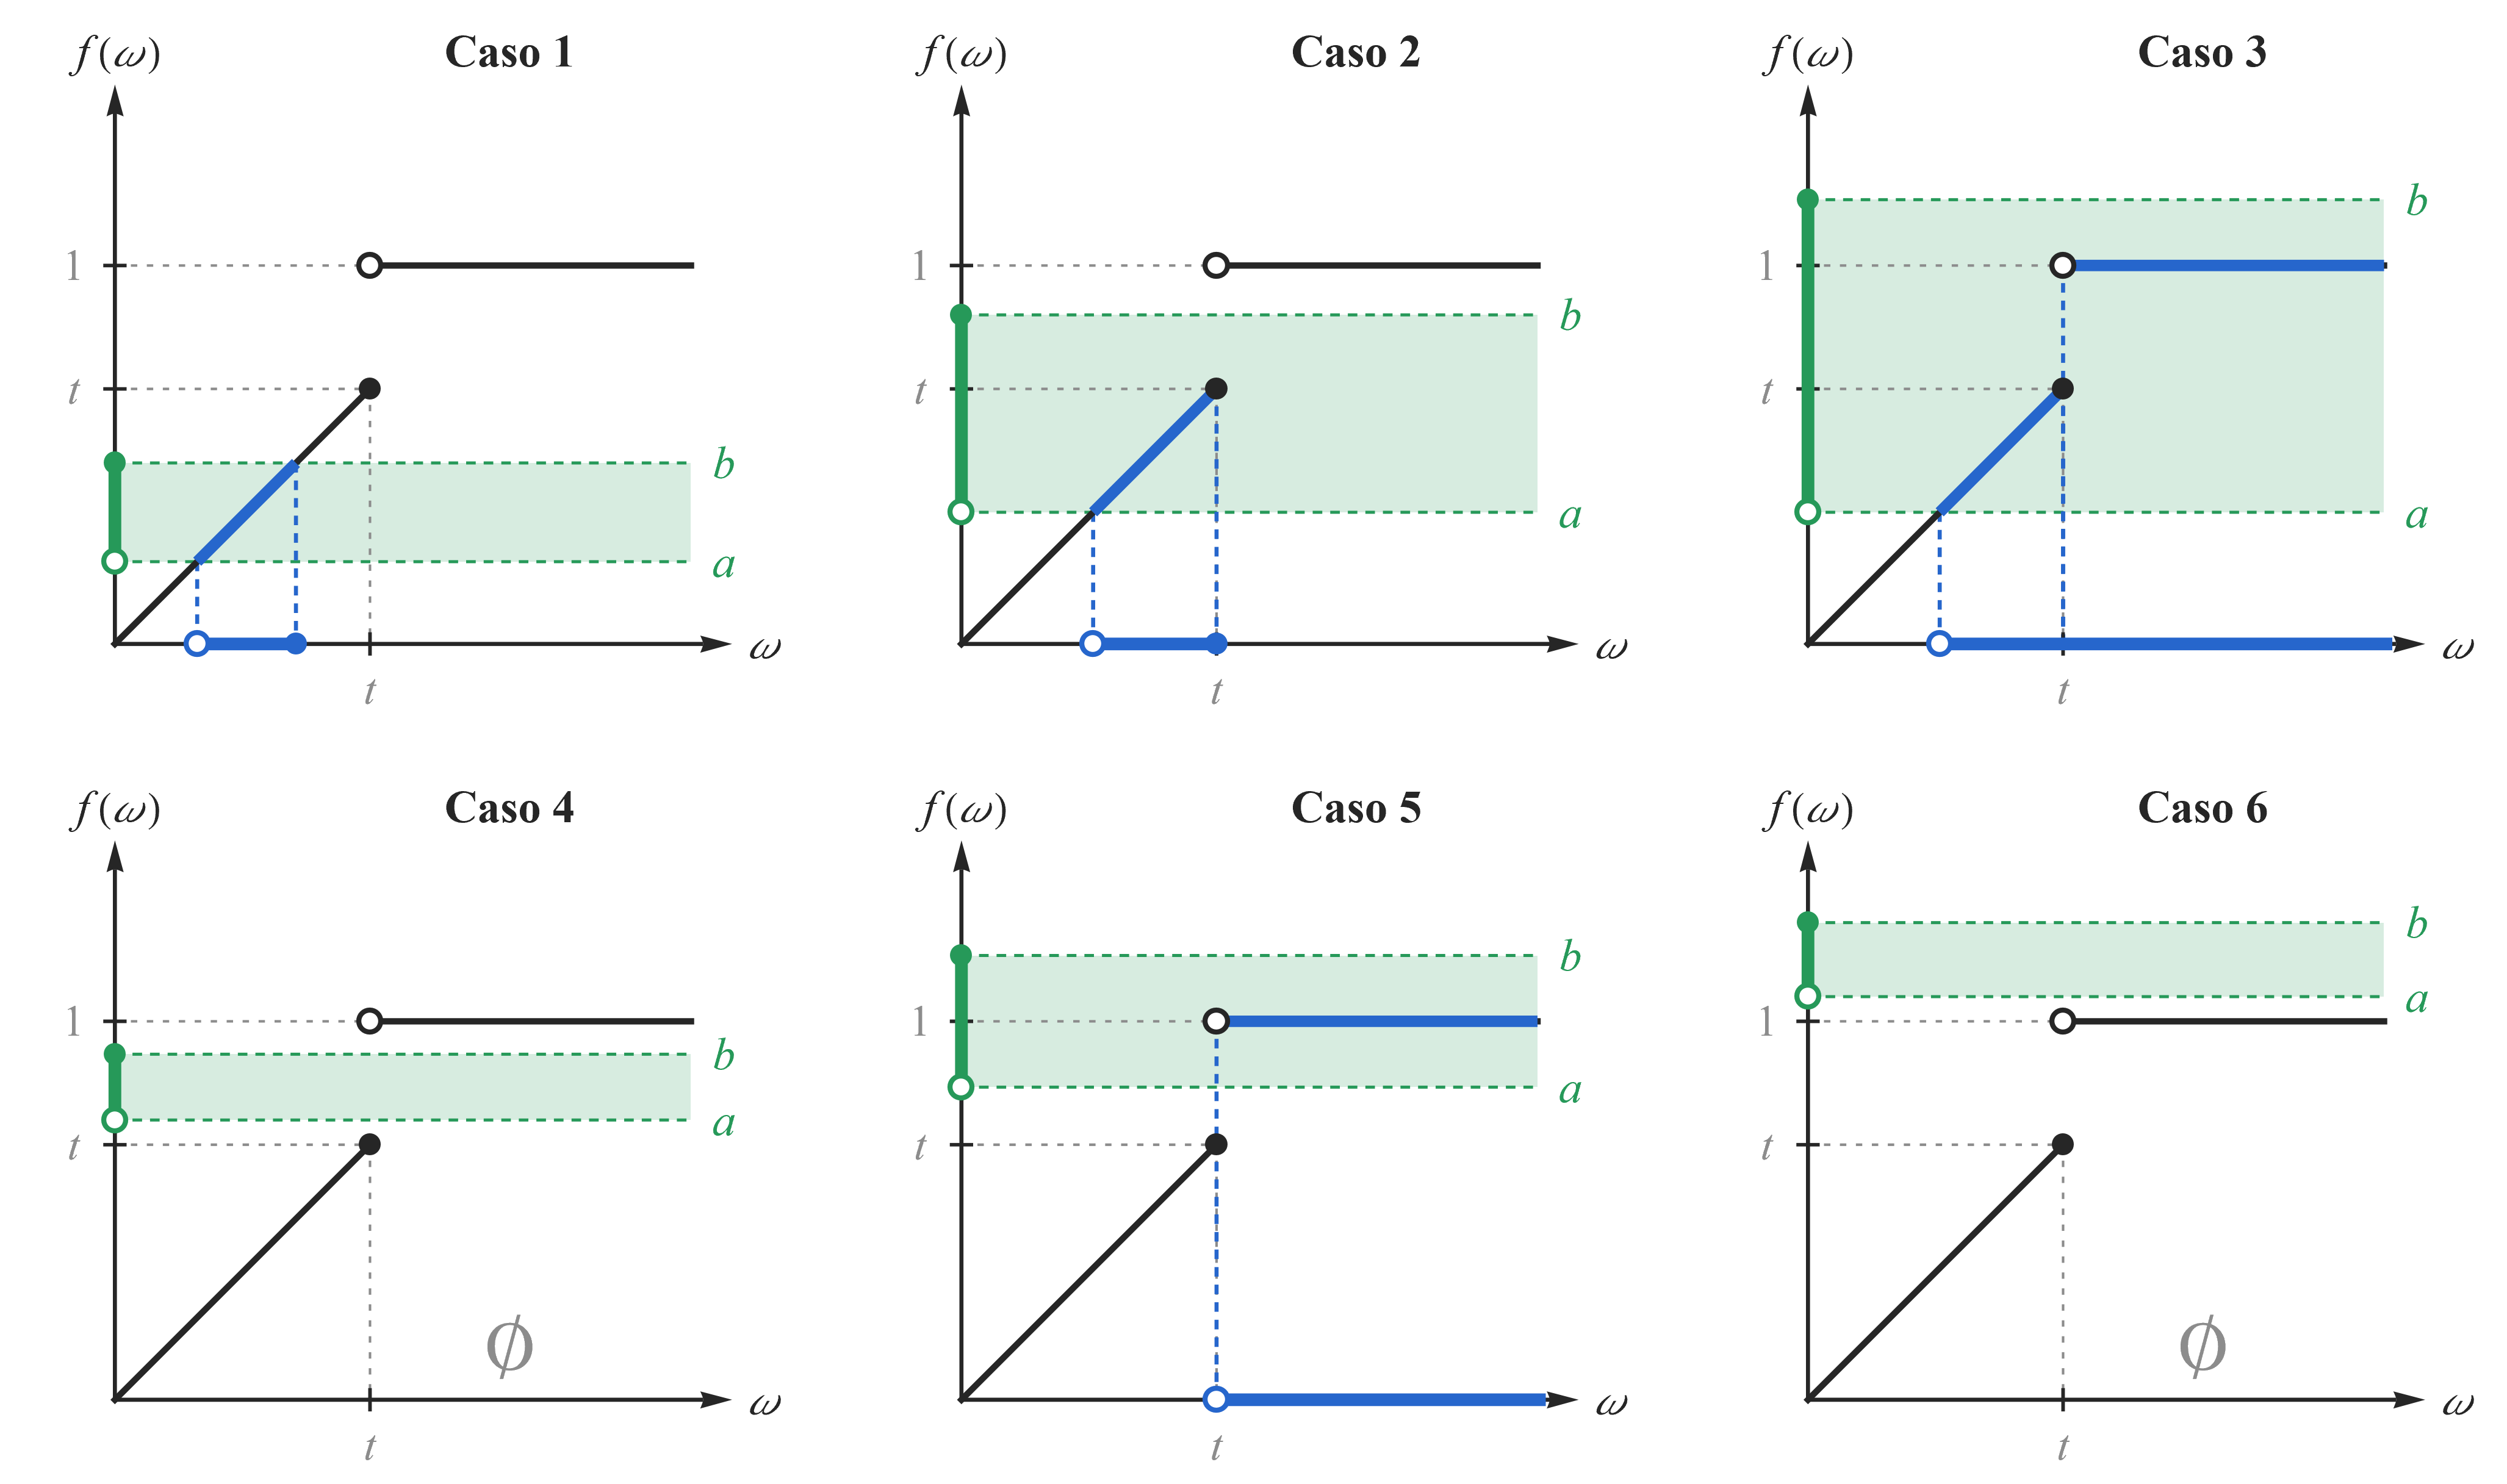
\includegraphics[width=0.95\linewidth]{imagenes/tema3/T3_P46_a.png}
\end{center}

\textbf{b) Análisis con la clase generadora $\mathcal{C}_2 = \{(-\infty, x] \mid x \in \mathbb{R}\}$:}

Calculamos la imagen inversa de las semirrectas $f^{-1}((-\infty, x])$ según el valor del parámetro $x$:

\begin{itemize}
    \item \textbf{Caso 1 ($x \le t$):}
    Para $\omega \le t$, $f(\omega) = \omega \in (-\infty, x] \iff \omega \le x$.
    Para $\omega > t$, $f(\omega) = 1 > t \ge x$, luego $1 \notin (-\infty, x]$.
    \[
        f^{-1}((-\infty, x]) = (-\infty, x] \in \mathcal{B}
    \]

    \item \textbf{Caso 2 ($t < x < 1$):}
    Para $\omega \le t$, $f(\omega) = \omega \le t < x$, por lo que todo $\omega \in (-\infty, t]$ verifica $f(\omega) \in (-\infty, x]$.
    Para $\omega > t$, $f(\omega) = 1 > x$, por lo que ningún $\omega > t$ está en el intervalo.
    \[
        f^{-1}((-\infty, x]) = (-\infty, t] \in \mathcal{B}
    \]

    \item \textbf{Caso 3 ($x \ge 1$):}
    Para $\omega \le t$, $f(\omega) = \omega \le t < 1 \le x$.
    Para $\omega > t$, $f(\omega) = 1 \le x$.
    Por tanto, todos los puntos de $\mathbb{R}$ verifican que su imagen pertenece a $(-\infty, x]$:
    \[
        f^{-1}((-\infty, x]) = (-\infty, t] \cup (t, \infty) = \mathbb{R} \in \mathcal{B}
    \]
\end{itemize}

\begin{center}
    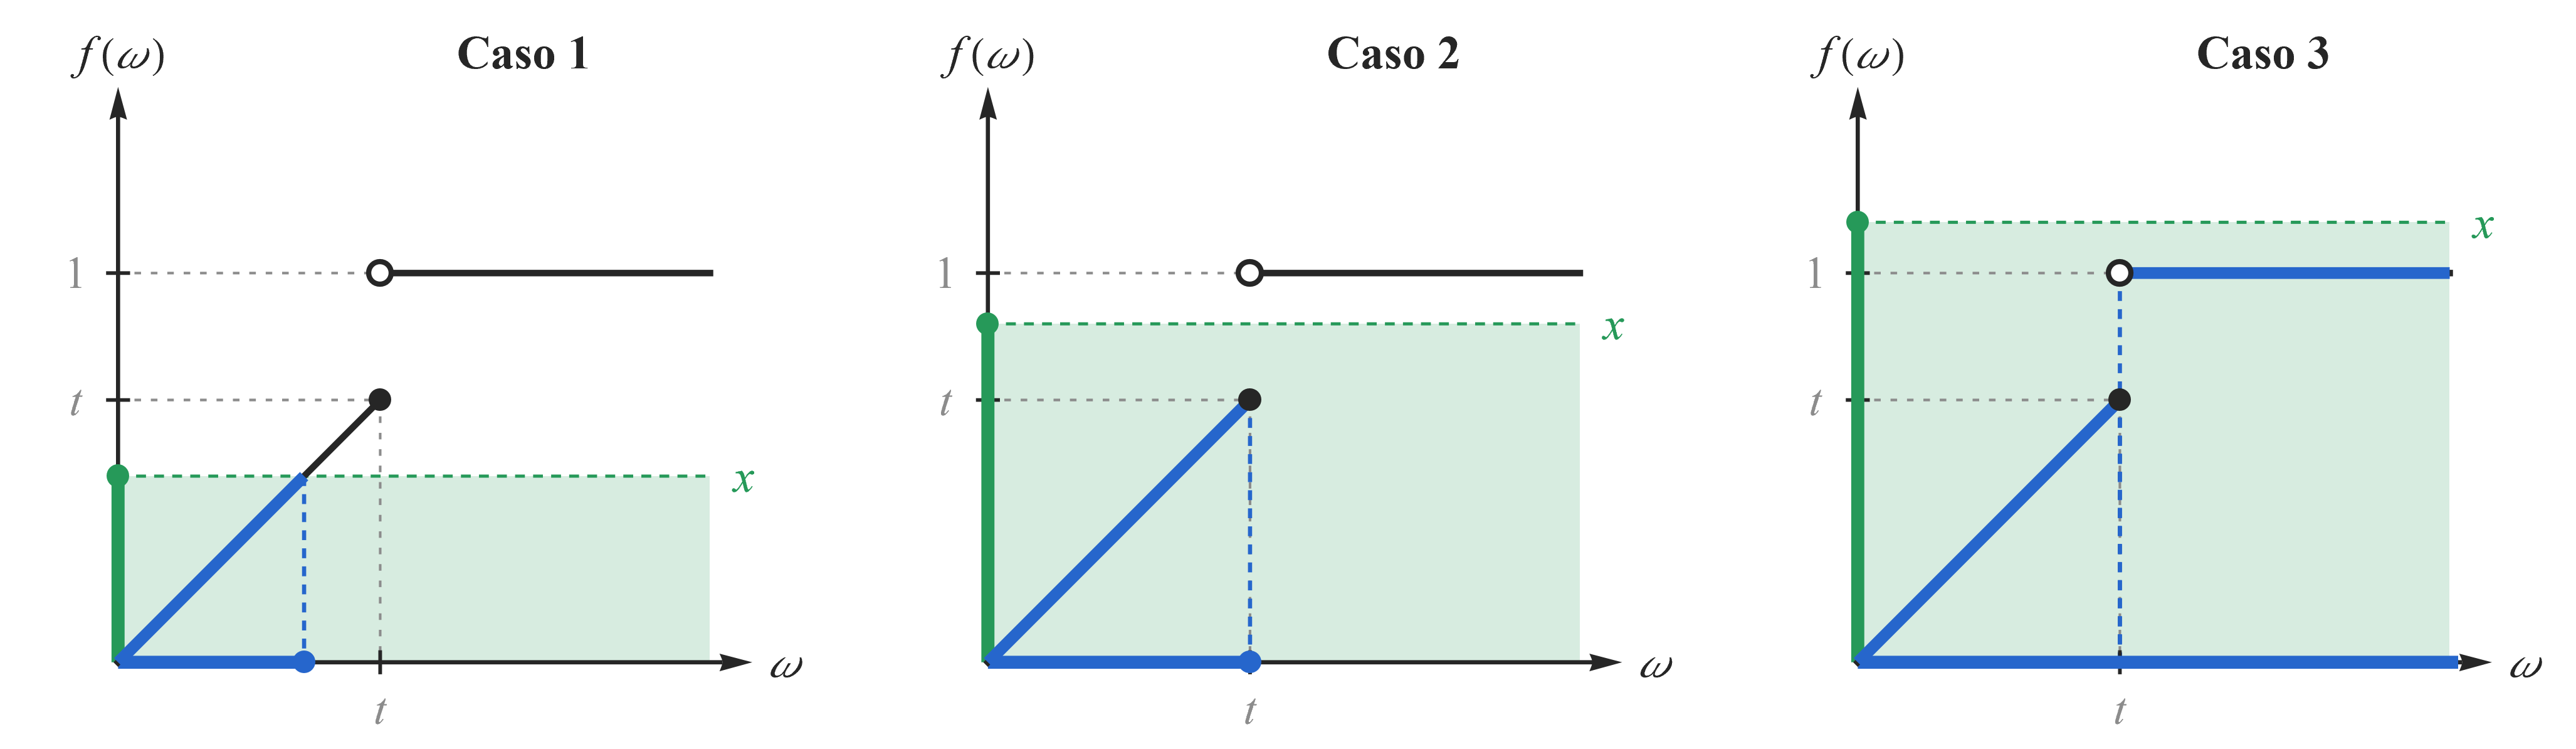
\includegraphics[width=0.95\linewidth]{imagenes/tema3/T3_P46_b.png}
\end{center}

Como $f^{-1}((-\infty, x]) \in \mathcal{B}$ para todo $x \in \mathbb{R}$, se confirma que \textbf{$f$ es una función medible}.
\end{problema}

\newpage
%===================
% Problema 47: 
%===================
\begin{problema}[Construcción de una función no medible con valor absoluto medible]
Construir una función $f : (\Omega, \mathcal{G}) \to (\mathbb{R}, \mathcal{B})$ que no sea medible, pero tal que su valor absoluto $|f| : (\Omega, \mathcal{G}) \to (\mathbb{R}, \mathcal{B})$ sí sea una función medible.

\tcblower

\paragraph{1. Construcción del espacio medible y de la función $f$:}
Sea $\Omega$ un conjunto no vacío y sea $A \subseteq \Omega$ un subconjunto propio no vacío ($\varnothing \neq A \neq \Omega$). Consideramos la $\sigma$-álgebra elemental generada por $A$:
\[
    \mathcal{G} = \sigma(\{A\}) = \{\Omega, \varnothing, A, A^c\}
\]

Seleccionamos un subconjunto propio no vacío $B \subsetneq A$ con $B \neq \varnothing$. Puesto que los únicos subconjuntos que pertenecen a $\mathcal{G}$ son $\{\Omega, \varnothing, A, A^c\}$ y $B \subsetneq A$, es evidente que $B \notin \mathcal{G}$.

Definimos la función $f : \Omega \to \mathbb{R}$ como:
\[
    f(\omega) = \begin{cases} -1 & \text{si } \omega \in B \\ 1 & \text{si } \omega \in A \setminus B \\ 0 & \text{si } \omega \in A^c \end{cases}
\]

\paragraph{2. Demostración de que $f$ no es medible:}
Para probar que $f$ no es medible respecto a $(\mathcal{G}, \mathcal{B})$, basta exhibir un conjunto boreliano $I \in \mathcal{B}$ cuya imagen inversa $f^{-1}(I)$ no pertenezca a $\mathcal{G}$.

Consideramos el intervalo boreliano $I = (-\infty, -1/2] \in \mathcal{B}$. Calculamos su antiimagen:
\[
    f^{-1}((-\infty, -1/2]) = \{\omega \in \Omega \mid f(\omega) \le -1/2\} = B
\]
Como $B \notin \mathcal{G}$, la imagen inversa de este boreliano no es un conjunto medible, lo que demuestra formalmente que \textbf{$f$ no es medible}.

\begin{center}
    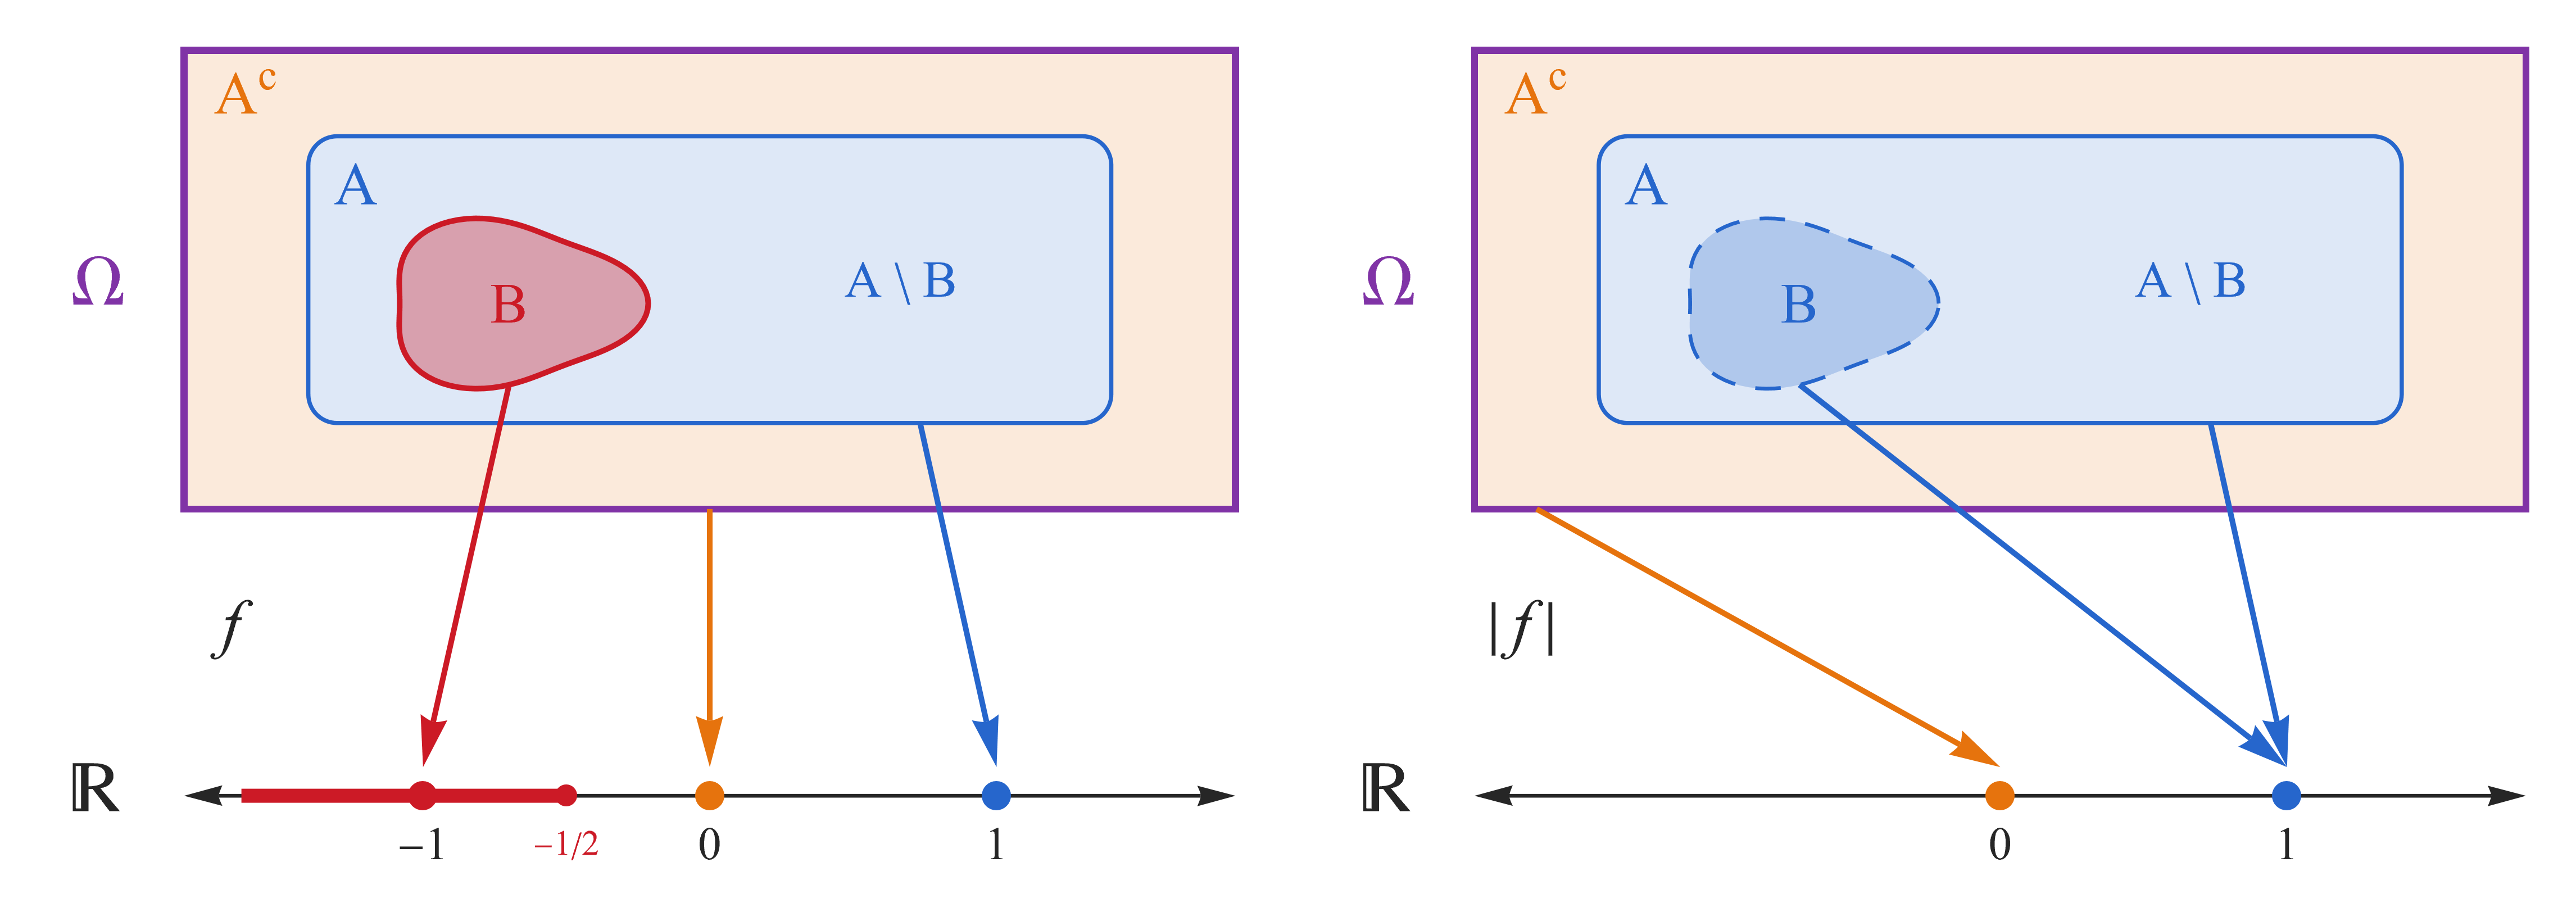
\includegraphics[width=0.95\linewidth]{imagenes/tema3/T3_P47_a.png}
\end{center}

\paragraph{3. Demostración de que $|f|$ es medible:}
Calculamos el valor absoluto $|f|(\omega) = |f(\omega)|$ para todo $\omega \in \Omega$:
\[
    |f|(\omega) = \begin{cases} |-1| = 1 & \text{si } \omega \in B \\ |1| = 1 & \text{si } \omega \in A \setminus B \\ |0| = 0 & \text{si } \omega \in A^c \end{cases} \implies |f|(\omega) = \begin{cases} 1 & \text{si } \omega \in A \\ 0 & \text{si } \omega \in A^c \end{cases} = \mathbf{1}_A(\omega)
\]

La función $|f|$ coincide con la función indicadora del conjunto $A$. Como por construcción $A \in \mathcal{G}$, la función característica $\mathbf{1}_A$ es una función simple medible.

Podemos verificarlo explícitamente evaluando la antiimagen de la clase generadora de semirrectas $\{(-\infty, x] \mid x \in \mathbb{R}\}$:
\[
    |f|^{-1}((-\infty, x]) = \begin{cases} 
        \varnothing \in \mathcal{G} & \text{si } x < 0 \\
        A^c \in \mathcal{G} & \text{si } 0 \le x < 1 \\
        \Omega \in \mathcal{G} & \text{si } x \ge 1 
    \end{cases}
\]

Dado que $|f|^{-1}((-\infty, x]) \in \mathcal{G}$ para todo $x \in \mathbb{R}$, queda demostrado que \textbf{$|f|$ es una función medible}.
\end{problema}

\newpage
%===================
% Problema 48: 
%===================
\begin{problema}[Teorema 10: Medida inducida por una aplicación medible]
Sea $f : (\Omega_1, \mathcal{G}_1, \mu) \to (\Omega_2, \mathcal{G}_2)$ una aplicación medible entre espacios medibles. Demostrar que la función de conjunto $\mu_f = \mu \circ f^{-1}$ define una medida sobre $(\Omega_2, \mathcal{G}_2)$. Demostrar asimismo que si $\mu$ es una medida de probabilidad, entonces $\mu_f$ es también una medida de probabilidad sobre $(\Omega_2, \mathcal{G}_2)$.

\tcblower

\paragraph{1. Buena definición de la función de conjunto $\mu_f$:}
Para que la composición $\mu_f(B) = (\mu \circ f^{-1})(B) = \mu(f^{-1}(B))$ esté bien definida para todo $B \in \mathcal{G}_2$, es imprescindible que la antiimagen $f^{-1}(B)$ pertenezca al dominio de la medida $\mu$, es decir, a la $\sigma$-álgebra $\mathcal{G}_1$.

Por hipótesis, $f : (\Omega_1, \mathcal{G}_1) \to (\Omega_2, \mathcal{G}_2)$ es una aplicación medible, lo que garantiza que $f^{-1}(B) \in \mathcal{G}_1$ para cualquier $B \in \mathcal{G}_2$. En consecuencia, $\mu_f : \mathcal{G}_2 \to \overline{\mathbb{R}}$ está correctamente definida.

\paragraph{2. Verificación de las propiedades de medida para $\mu_f$:}
Comprobamos los tres axiomas constitutivos de una medida sobre $(\Omega_2, \mathcal{G}_2)$:

\begin{enumerate}[label=\arabic*.]
    \item \textbf{No negatividad:}
    Para todo suceso medible $B \in \mathcal{G}_2$, dado que $f^{-1}(B) \in \mathcal{G}_1$ y la medida $\mu$ es no negativa:
    \[
        \mu_f(B) = \mu(f^{-1}(B)) \ge 0, \quad \forall B \in \mathcal{G}_2
    \]

    \item \textbf{Medida del conjunto vacío:}
    Aprovechando que $f^{-1}(\varnothing) = \varnothing$ y que $\mu(\varnothing) = 0$ por ser $\mu$ una medida:
    \[
        \mu_f(\varnothing) = \mu(f^{-1}(\varnothing)) = \mu(\varnothing) = 0
    \]

    \item \textbf{$\sigma$-aditividad:}
    Sea $(B_n)_{n \in \mathbb{N}} \subseteq \mathcal{G}_2$ una sucesión de conjuntos disjuntos dos a dos ($B_i \cap B_j = \varnothing$ para todo $i \neq j$).
    Por las propiedades de la imagen inversa, las antiimágenes resultan también mutuamente disjuntas en $\Omega_1$:
    \[
        f^{-1}(B_i) \cap f^{-1}(B_j) = f^{-1}(B_i \cap B_j) = f^{-1}(\varnothing) = \varnothing, \quad \forall i \neq j
    \]
    Intercambiando la unión numerable con la imagen inversa y aplicando la $\sigma$-aditividad de la medida $\mu$ sobre la sucesión disjunta $(f^{-1}(B_n))_{n \in \mathbb{N}} \subseteq \mathcal{G}_1$:
    \[
        \mu_f\left( \bigsqcup_{n=1}^\infty B_n \right) = \mu\left( f^{-1}\left( \bigsqcup_{n=1}^\infty B_n \right) \right) = \mu\left( \bigsqcup_{n=1}^\infty f^{-1}(B_n) \right) = \sum_{n=1}^\infty \mu(f^{-1}(B_n)) = \sum_{n=1}^\infty \mu_f(B_n)
    \]
\end{enumerate}

Por lo tanto, $\mu_f$ es una medida sobre $(\Omega_2, \mathcal{G}_2)$.

% Espacio reservado para incorporar diagrama explicativo en los apuntes
\begin{center}
    \vspace{0.2cm}
    \framebox[\linewidth]{\vbox to 2.2cm{\vfill \centering \textit{[Espacio reservado para diagrama: Esquema del transporte de la medida $\mu$ desde $\Omega_1$ hacia $\Omega_2$ mediante la función de conjunto $\mu_f = \mu \circ f^{-1}$]} \vfill}}
    \vspace{0.2cm}
\end{center}

\paragraph{3. Conservación de la condición de medida de probabilidad:}
Si la medida original $\mu$ es una probabilidad sobre $\Omega_1$, satisface el axioma de normalización $\mu(\Omega_1) = 1$.

Evaluamos la medida inducida $\mu_f$ sobre el espacio muestral de llegada $\Omega_2$:
\[
    \mu_f(\Omega_2) = \mu(f^{-1}(\Omega_2)) = \mu(\Omega_1) = 1
\]

Por lo tanto, $\mu_f$ es una medida de probabilidad sobre $(\Omega_2, \mathcal{G}_2)$.
\end{problema}

\newpage
%===================
% Problema 49: 
%===================
\begin{problema}[Medibilidad y medida inducida por una función constante a trozos y afín]
Sea $\lambda$ la medida de Lebesgue sobre $(\mathbb{R}, \mathcal{B})$. Se define la función $f : (\mathbb{R}, \mathcal{B}, \lambda) \to ([0, 12], \mathcal{B}_{[0,12]})$ por:
\[
    f(\omega) = \begin{cases} 0 & \text{si } \omega < 0 \\ 2\omega + 1 & \text{si } 0 \le \omega < 5 \\ 12 & \text{si } 5 \le \omega \end{cases}
\]
\begin{enumerate}[label=\alph*)]
    \item Demostrar que $f$ es una función medible utilizando como clase generadora de $\mathcal{B}_{[0,12]}$ las semirrectas de la forma $(-\infty, x] \cap [0,12]$ con $x \in [0, 12]$.
    \item Calcular la medida inducida $\mu_f = \lambda \circ f^{-1}$ sobre la clase generadora de intervalos $(a,b] \subseteq [0, 12]$ y determinar la medida del intervalo $\mu_f([1, 6])$.
\end{enumerate}

\tcblower

\textbf{a) Estudio de la medibilidad de $f$ mediante la clase generadora de semirrectas:}

Analizamos la imagen directa de la función $f$, la cual viene dada por $\mathrm{Im}(f) = \{0\} \cup [1, 11) \cup \{12\}$.

Consideramos la clase generadora $\mathcal{C} = \{(-\infty, x] \cap [0,12] \mid x \in [0, 12]\}$, que genera la $\sigma$-álgebra de Borel restringida $\mathcal{B}_{[0,12]}$. Calculamos la antiimagen $f^{-1}((-\infty, x])$ para cada valor del parámetro $x \in [0, 12]$:

\begin{itemize}
    \item \textbf{Si $0 \le x < 1$:} Únicamente el valor $0 \in \mathrm{Im}(f)$ pertenece al intervalo $(-\infty, x]$. Como $f(\omega) = 0 \iff \omega < 0$:
    \[
        f^{-1}((-\infty, x]) = (-\infty, 0) \in \mathcal{B}
    \]
    \item \textbf{Si $1 \le x < 11$:} El intervalo $(-\infty, x]$ contiene al valor $0$ y al tramo continuo $[1, x]$. Resolviendo $2\omega + 1 \le x \iff \omega \le \frac{x-1}{2}$:
    \[
        f^{-1}((-\infty, x]) = (-\infty, 0) \cup \left[0, \frac{x-1}{2}\right] = \left(-\infty, \frac{x-1}{2}\right] \in \mathcal{B}
    \]
    \item \textbf{Si $11 \le x < 12$:} El intervalo $(-\infty, x]$ contiene a $0$ y a todo el tramo $[1, 11)$, pero no al punto $12$. Como $f(\omega) < 11 \iff \omega < 5$:
    \[
        f^{-1}((-\infty, x]) = (-\infty, 5) \in \mathcal{B}
    \]
    \item \textbf{Si $x = 12$:} Contiene a toda la imagen $\mathrm{Im}(f)$, por lo que la antiimagen es el espacio total:
    \[
        f^{-1}((-\infty, 12]) = \mathbb{R} \in \mathcal{B}
    \]
\end{itemize}

Puesto que todas las antiimágenes pertenecen a la $\sigma$-álgebra de Borel $\mathcal{B}$, por el Corolario de las clases generadoras se concluye que \textbf{$f$ es una función medible}.

\textbf{b) Expresión de la medida inducida $\mu_f = \lambda \circ f^{-1}$ y cálculo de $\mu_f([1, 6])$:}

\paragraph{1. Cálculo de la medida inducida $\mu_f((a, b]) = \lambda(f^{-1}((a, b]))$ para $a < b$:}
Analizamos las antiimágenes y sus medidas de Lebesgue según los valores de los extremos $a$ y $b$:
\begin{itemize}
    \item \textbf{Si $a < 0 \le b$:} El punto $0 \in (a, b]$, luego $f^{-1}((a,b])$ contiene a $(-\infty, 0)$, resultando:
    \[
        \mu_f((a, b]) = \lambda((-\infty, 0) \cup \dots) = \infty
    \]
    \item \textbf{Si $0 \le a < b < 1$:} El intervalo $(a, b]$ no contiene puntos de $\mathrm{Im}(f)$, luego $f^{-1}((a,b]) = \varnothing$ y:
    \[
        \mu_f((a, b]) = \lambda(\varnothing) = 0
    \]
    \item \textbf{Si $0 \le a < 1$ y $1 \le b < 11$:} $f^{-1}((a, b]) = \left[0, \frac{b-1}{2}\right]$, por lo que:
    \[
        \mu_f((a, b]) = \lambda\left(\left[0, \frac{b-1}{2}\right]\right) = \frac{b-1}{2}
    \]
    \item \textbf{Si $0 \le a < 1$ y $11 \le b < 12$:} $f^{-1}((a, b]) = [0, 5)$, por lo que:
    \[
        \mu_f((a, b]) = \lambda([0, 5)) = 5
    \]
    \item \textbf{Si $1 \le a < b < 11$:} $f^{-1}((a, b]) = \left(\frac{a-1}{2}, \frac{b-1}{2}\right]$, por lo que:
    \[
        \mu_f((a, b]) = \lambda\left(\left(\frac{a-1}{2}, \frac{b-1}{2}\right]\right) = \frac{b-1}{2} - \frac{a-1}{2} = \frac{b-a}{2}
    \]
    \item \textbf{Si $1 \le a < 11$ y $11 \le b < 12$:} $f^{-1}((a, b]) = \left(\frac{a-1}{2}, 5\right)$, por lo que:
    \[
        \mu_f((a, b]) = \lambda\left(\left(\frac{a-1}{2}, 5\right)\right) = 5 - \frac{a-1}{2} = \frac{11-a}{2}
    \]
    \item \textbf{Si $11 \le a < b < 12$:} El intervalo no contiene puntos de $\mathrm{Im}(f)$, luego $f^{-1}((a,b]) = \varnothing$ y:
    \[
        \mu_f((a, b]) = 0
    \]
    \item \textbf{Si $b \ge 12$ (con $a < 12$):} El punto $12 \in (a, b]$, por lo que $f^{-1}((a,b])$ contiene a $[5, \infty)$, de donde:
    \[
        \mu_f((a, b]) = \lambda([5, \infty) \cup \dots) = \infty
    \]
\end{itemize}

\paragraph{2. Cálculo de $\mu_f([1, 6])$:}
El intervalo $[1, 6]$ es un conjunto medible de $\mathcal{B}_{[0,12]}$. Calculamos directamente su antiimagen por la función $f$:
\[
    f^{-1}([1, 6]) = \{\omega \in \mathbb{R} \mid 1 \le f(\omega) \le 6\} = \{\omega \in \mathbb{R} \mid 1 \le 2\omega + 1 \le 6\} = \left[0, \frac{5}{2}\right]
\]
Por la definición de la medida inducida $\mu_f = \lambda \circ f^{-1}$:
\[
    \mu_f([1, 6]) = \lambda(f^{-1}([1, 6])) = \lambda\left(\left[0, \frac{5}{2}\right]\right) = \frac{5}{2} = 2.5
\]

\textit{Cálculo alternativo mediante continuidad descendente:}
Consideramos la sucesión decreciente de intervalos $(1 - 1/n, 6] \downarrow [1, 6]$ cuando $n \to \infty$. Para cada $n \ge 1$, el extremo inferior cumple $0 \le 1 - 1/n < 1$ y el extremo superior $1 \le 6 < 11$. Aplicando la fórmula obtenida anteriormente:
\[
    \mu_f((1 - 1/n, 6]) = \frac{6 - 1}{2} = 2.5, \quad \forall n \ge 1
\]
Tomando el límite cuando $n \to \infty$ por continuidad descendente de la medida sobre la sucesión de conjuntos de medida finita:
\[
    \mu_f([1, 6]) = \lim_{n \to \infty} \mu_f((1 - 1/n, 6]) = \lim_{n \to \infty} 2.5 = 2.5
\]
\end{problema}
\newpage
%===================
% Problema 49 (Apartado c): 
%===================
\begin{problema}[Medibilidad mediante la clase generadora de intervalos \texorpdfstring{$(a,b]$}{(a,b]}]
Sea $\lambda$ la medida de Lebesgue sobre $(\mathbb{R}, \mathcal{B})$. Se considera la función $f : (\mathbb{R}, \mathcal{B}, \lambda) \to ([0, 12], \mathcal{B}_{[0,12]})$ definida por:
\[
    f(\omega) = \begin{cases} 
        0 & \text{si } \omega < 0 \\ 
        2\omega + 1 & \text{si } 0 \le \omega < 5 \\ 
        12 & \text{si } 5 \le \omega 
    \end{cases}
\]
Demostrar que $f$ es una función medible utilizando como clase generadora de $\mathcal{B}$ los intervalos de la forma $(a,b]$ con $a, b \in \mathbb{R}$ y $a < b$.

\tcblower

Para demostrar que $f$ es medible respecto a la $\sigma$-álgebra de Borel restringida $\mathcal{B}_{[0,12]}$, utilizamos la clase generadora habitual de $\mathcal{B}$:
\[
    \mathcal{C} = \{ (a, b] \mid a, b \in \mathbb{R}, \, a < b \}
\]
La traza de esta clase generadora sobre el espacio de llegada $[0, 12]$ viene dada por:
\[
    \mathcal{C}_{[0,12]} = \mathcal{C} \cap [0, 12] = \{ (a, b] \cap [0, 12] \mid a, b \in \mathbb{R}, \, a < b \}
\]
Dado que $\sigma(\mathcal{C}) = \mathcal{B}$, el Teorema Referencial garantiza que $\sigma_{[0,12]}(\mathcal{C}_{[0,12]}) = \mathcal{B}_{[0,12]}$. Por el Corolario de las clases generadoras, basta comprobar que para todo elemento de la traza $I \in \mathcal{C}_{[0,12]}$, su imagen inversa satisface $f^{-1}(I) \in \mathcal{B}$.

Recordamos que la imagen directa de la función es $\mathrm{Im}(f) = \{0\} \cup [1, 11) \cup \{12\}$.

\begin{center}
    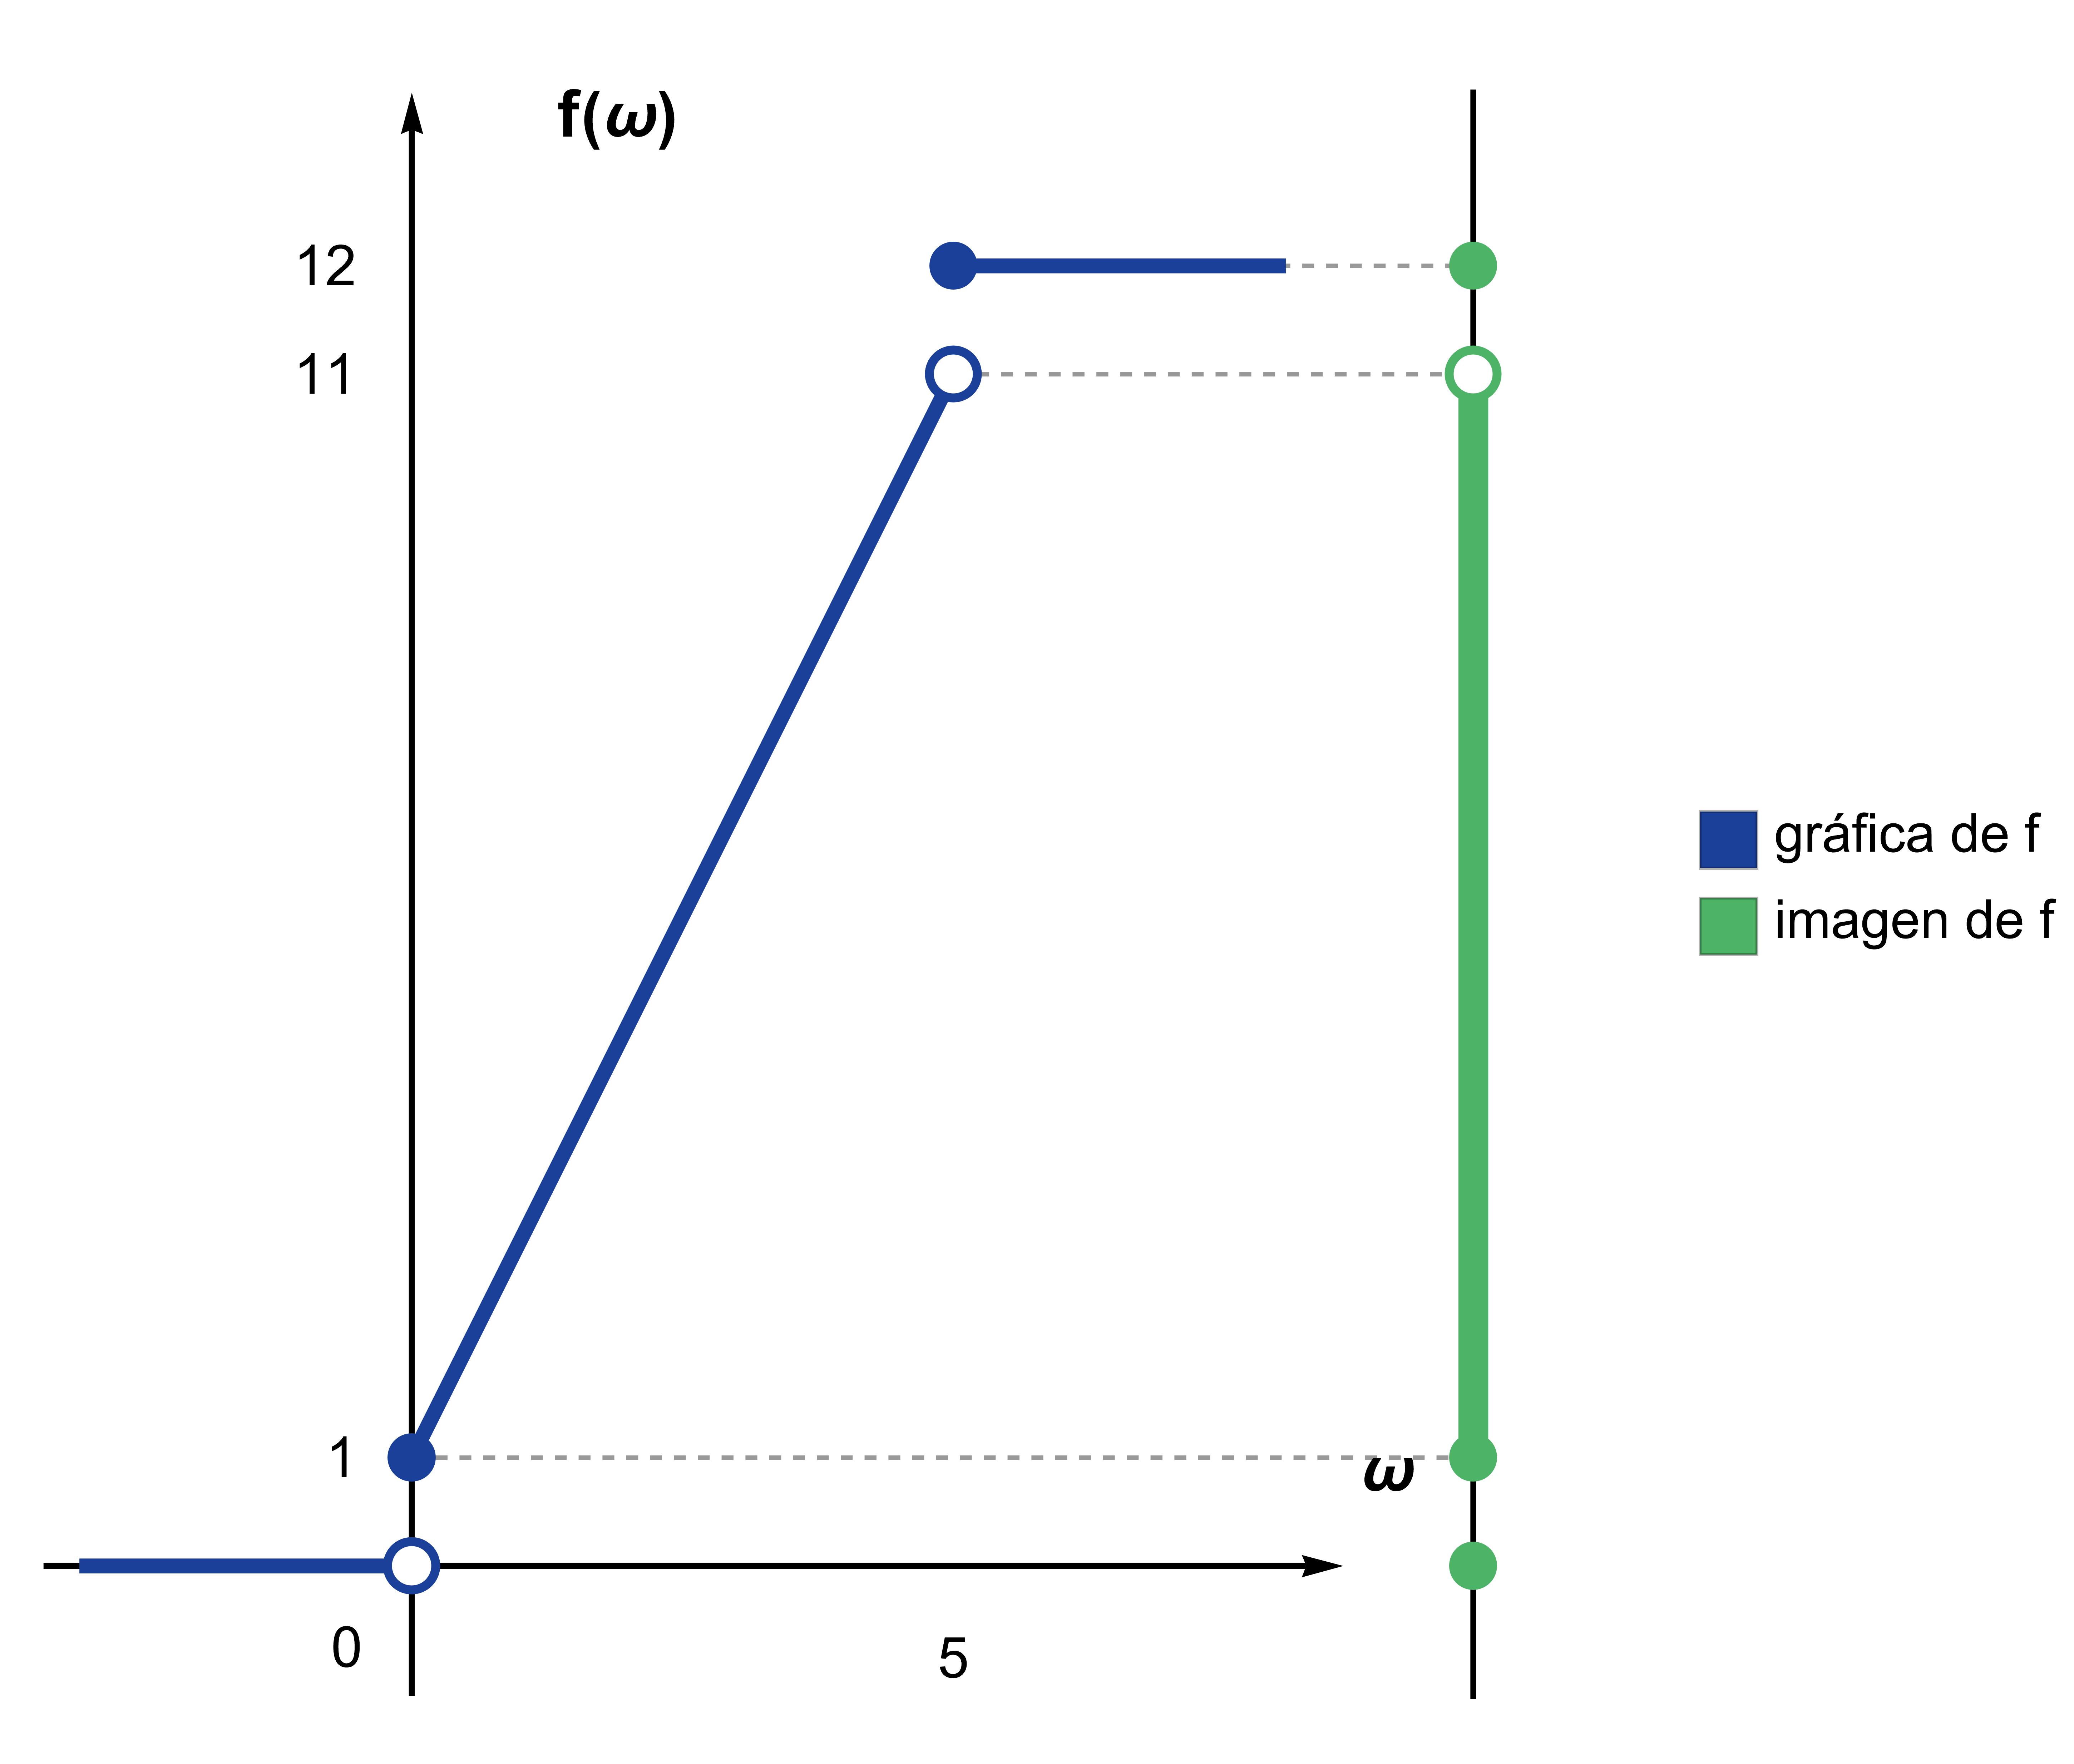
\includegraphics[width=0.65\linewidth]{imagenes/tema3/T3_P49_funcion.png}
\end{center}

\newpage
Analizamos la antiimagen $f^{-1}((a,b] \cap [0,12])$ distinguiendo todos los casos posibles según la posición de los extremos $a$ y $b$:

\paragraph{1. Casos con $a < 0$ (la traza sobre $[0, 12]$ contiene al origen $0$):}
En este bloque, $(a,b] \cap [0,12] = [0, \min(b, 12)]$:
\begin{itemize}
    \item \textbf{Caso 1 ($b \le 0$):} $(a,b] \cap [0,12] = \varnothing \implies f^{-1}(\varnothing) = \varnothing \in \mathcal{B}$.
    \begin{center}
        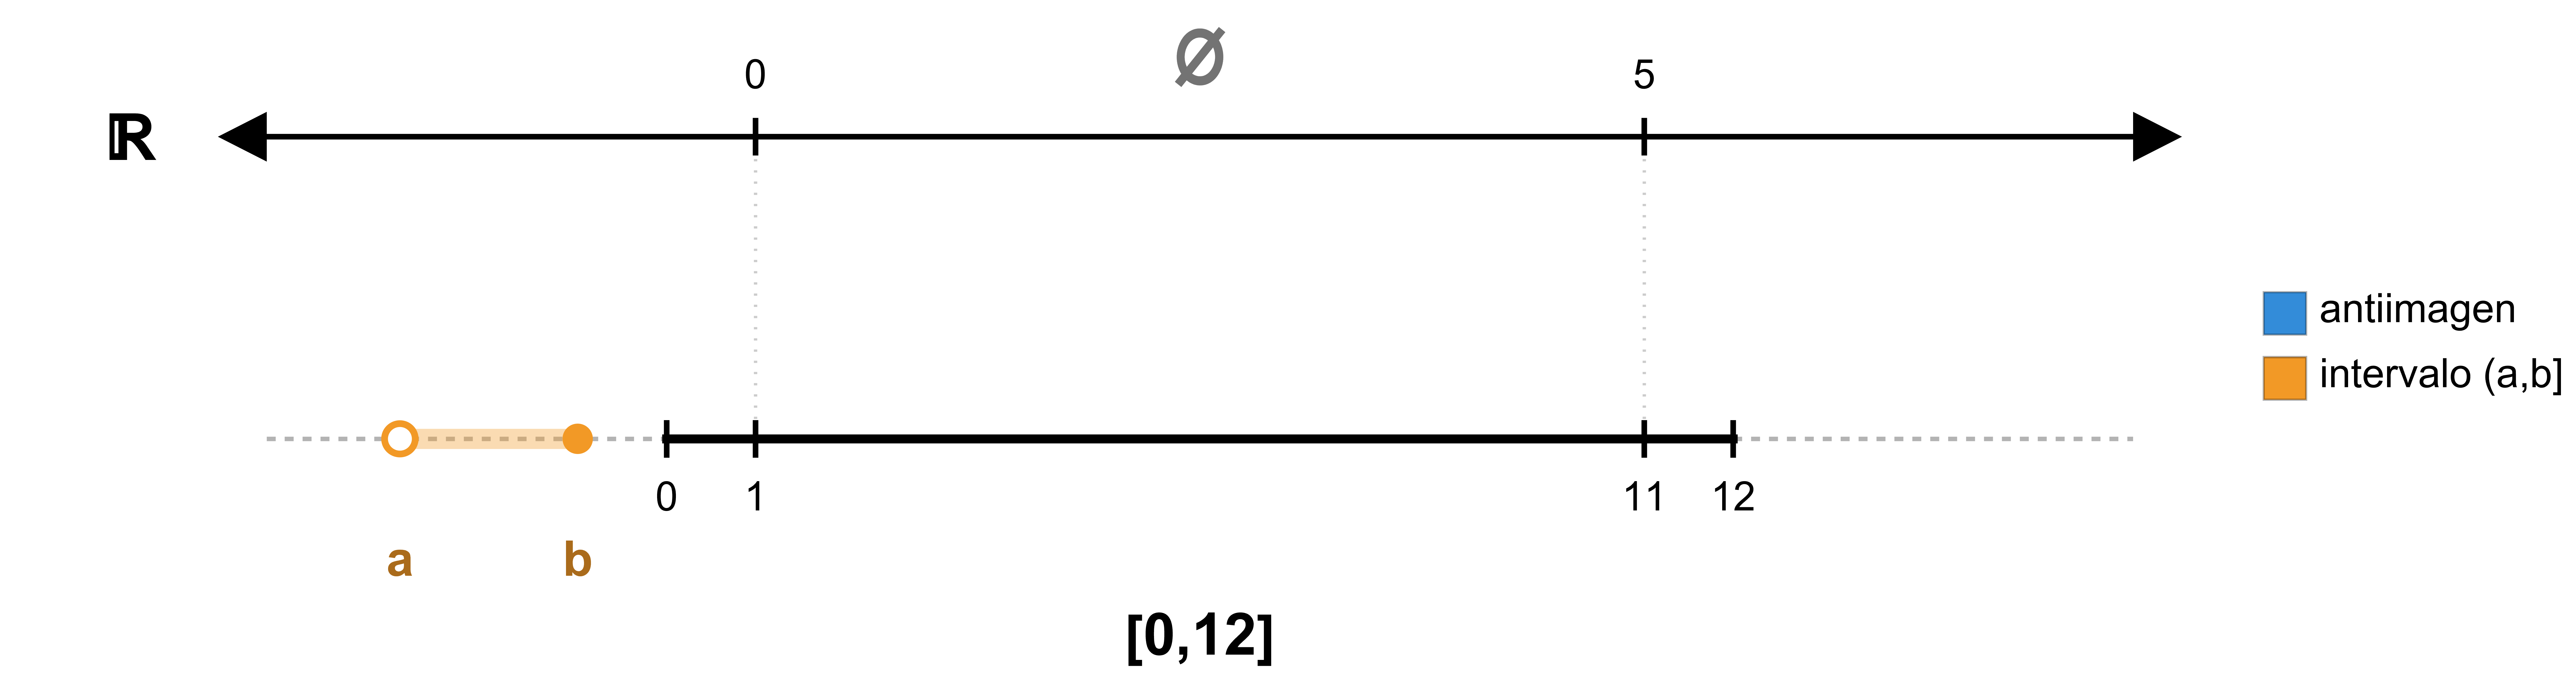
\includegraphics[width=0.75\linewidth]{imagenes/tema3/T3_P49_c01.png}
    \end{center}

    \item \textbf{Caso 2 ($0 \le b < 1$):} $[0,b] \cap \mathrm{Im}(f) = \{0\} \implies f^{-1}(\{0\}) = (-\infty, 0) \in \mathcal{B}$.
    \begin{center}
        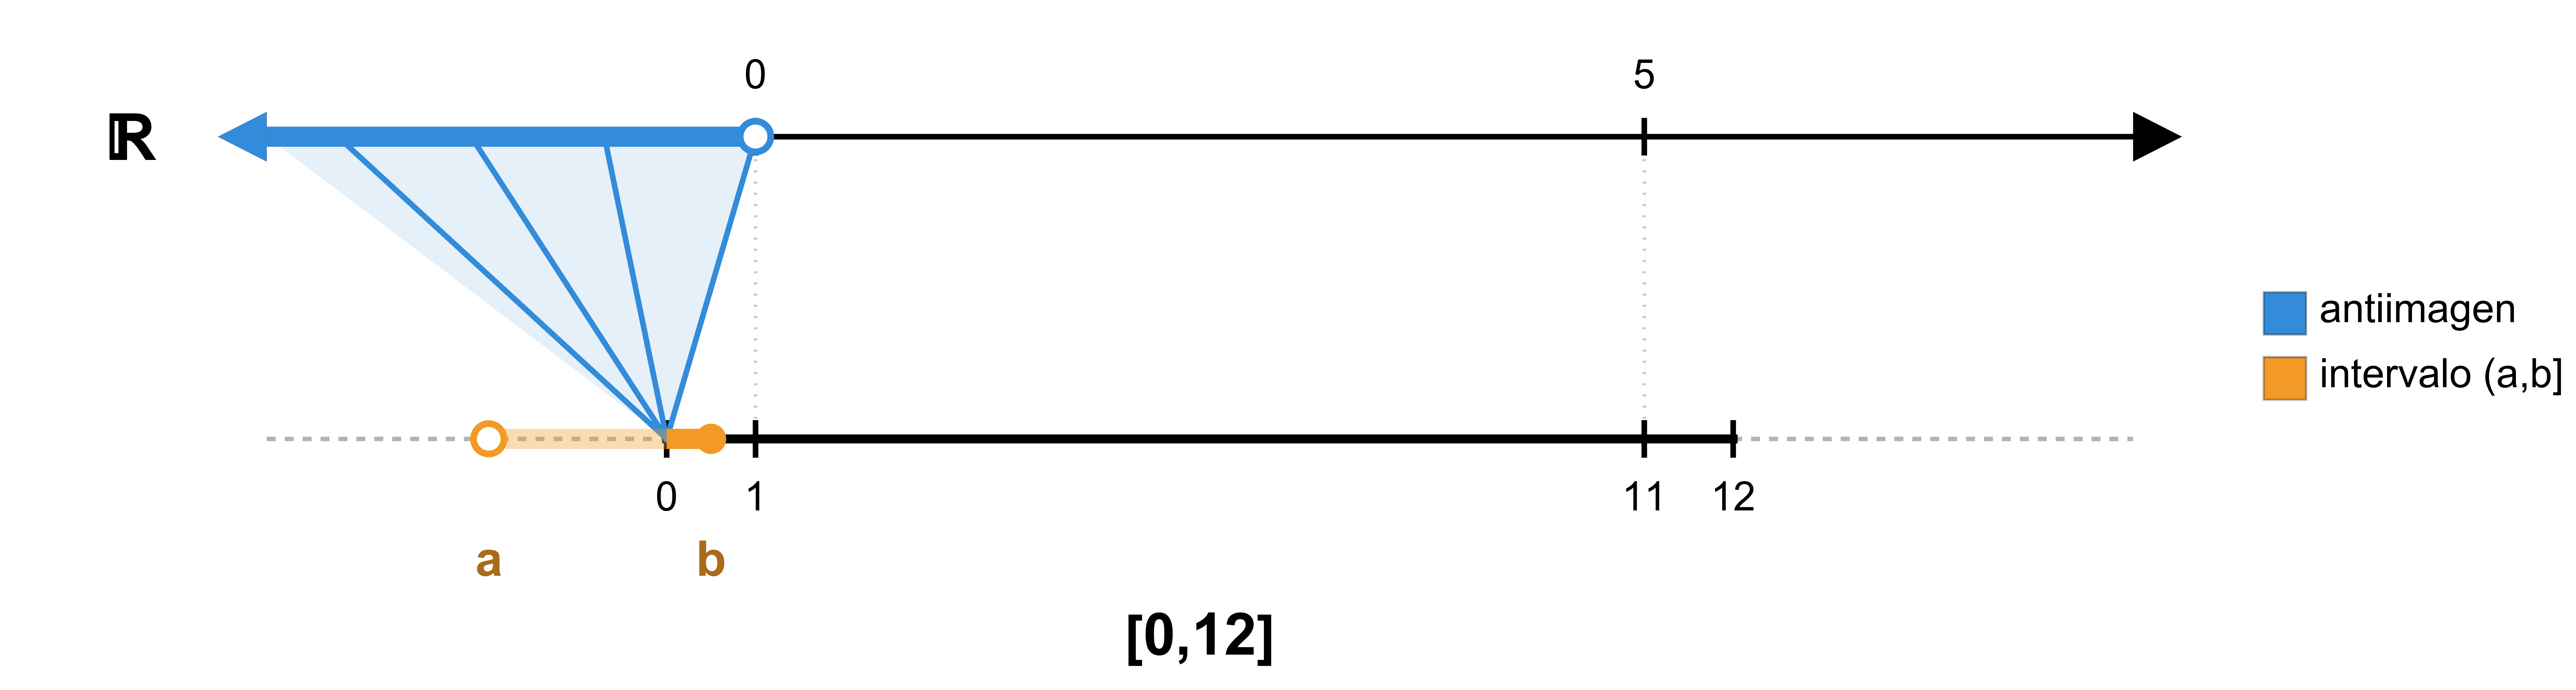
\includegraphics[width=0.75\linewidth]{imagenes/tema3/T3_P49_c02.png}
    \end{center}

    \item \textbf{Caso 3 ($1 \le b < 11$):} $[0,b] \cap \mathrm{Im}(f) = \{0\} \cup [1,b] \implies \\
    \implies f^{-1}(\{0\}) \cup f^{-1}([1,b]) = (-\infty, 0) \cup \left[0, \frac{b-1}{2}\right] = \left(-\infty, \frac{b-1}{2}\right] \in \mathcal{B}$.
    \begin{center}
        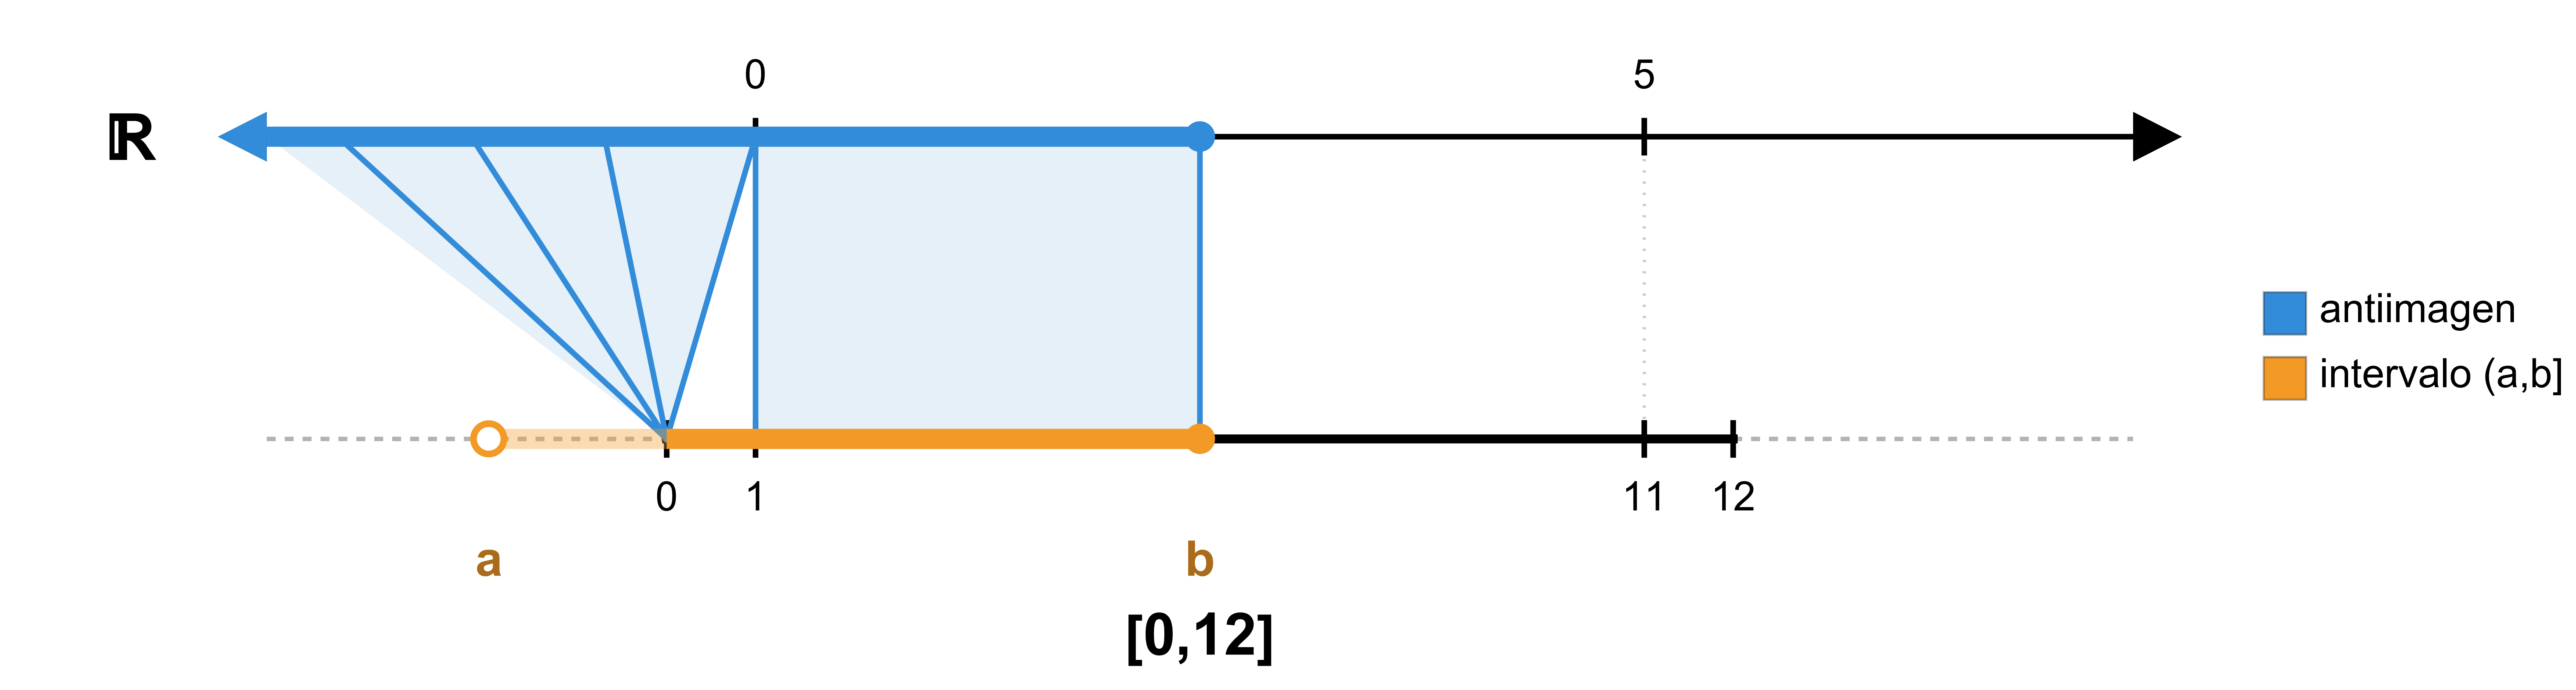
\includegraphics[width=0.75\linewidth]{imagenes/tema3/T3_P49_c03.png}
    \end{center}

    \item \textbf{Caso 4 ($11 \le b < 12$):} $[0,b] \cap \mathrm{Im}(f) = \{0\} \cup [1,11) \implies \\
    \implies f^{-1}(\{0\}) \cup f^{-1}([1,11)) = (-\infty, 0) \cup [0, 5) = (-\infty, 5) \in \mathcal{B}$.
    \begin{center}
        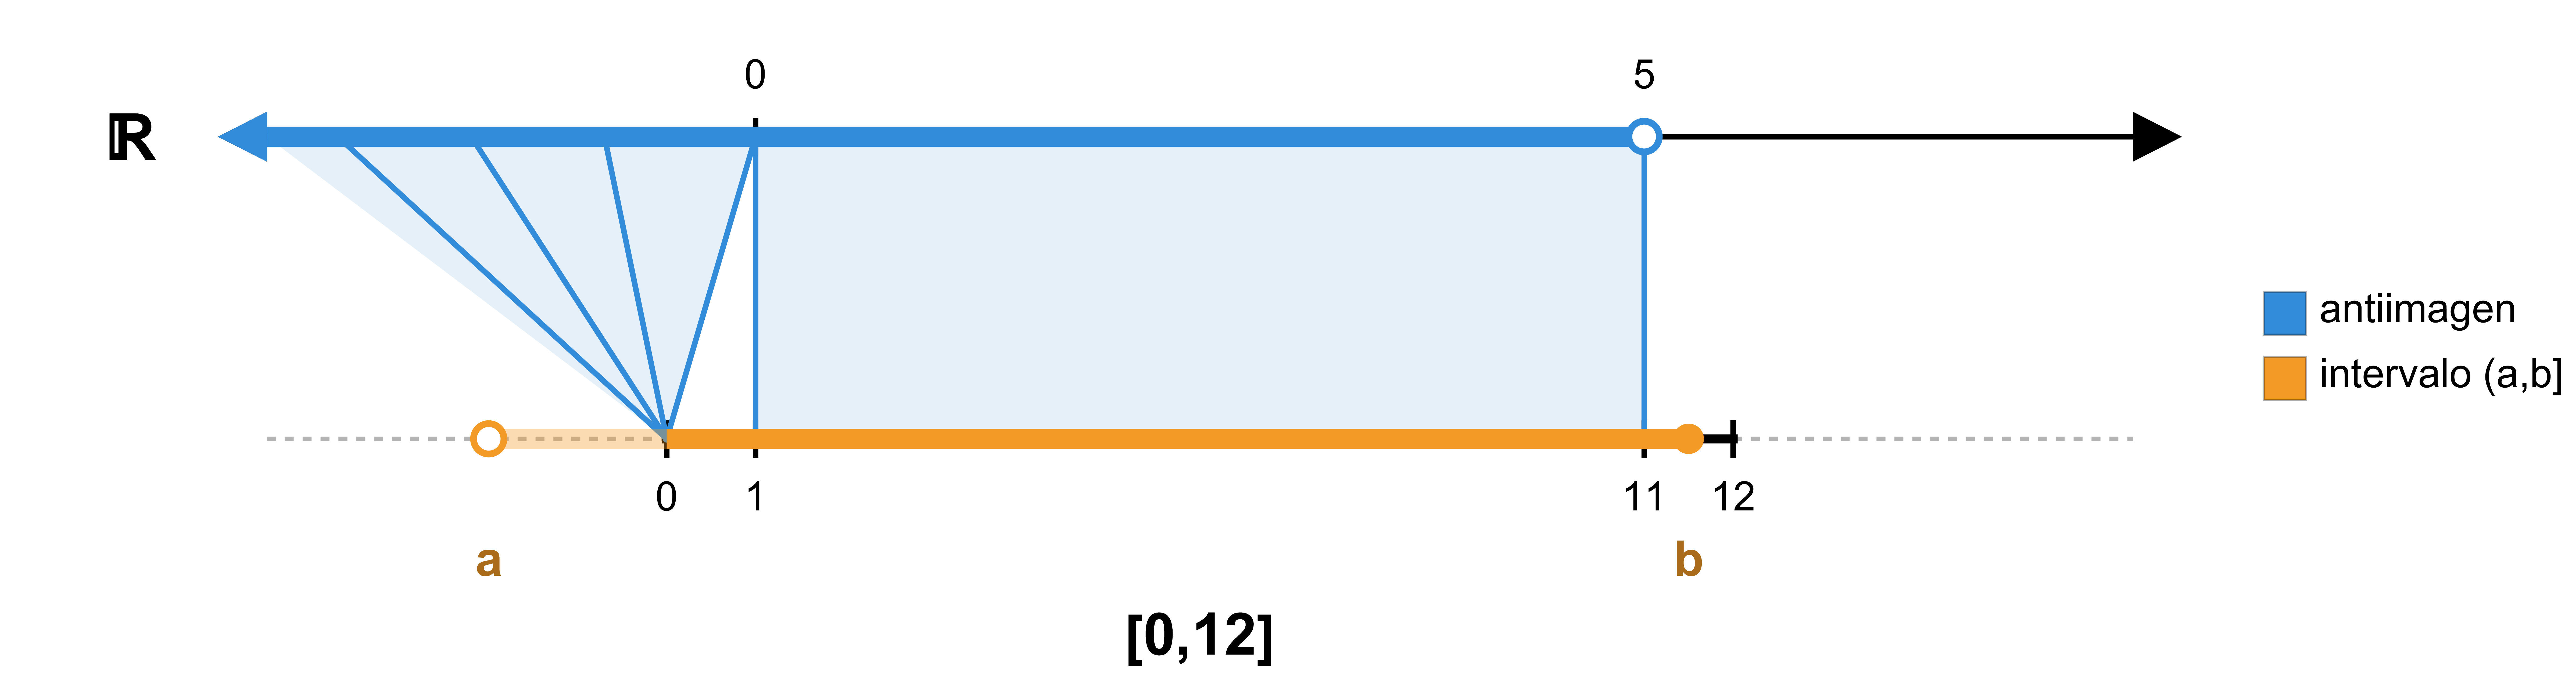
\includegraphics[width=0.75\linewidth]{imagenes/tema3/T3_P49_c04.png}
    \end{center}

    \item \textbf{Caso 5 ($b \ge 12$):} $[0,12] \cap \mathrm{Im}(f) = \mathrm{Im}(f) \implies \\
    \implies f^{-1}([0,12]) = \mathbb{R} \in \mathcal{B}$.
    \begin{center}
        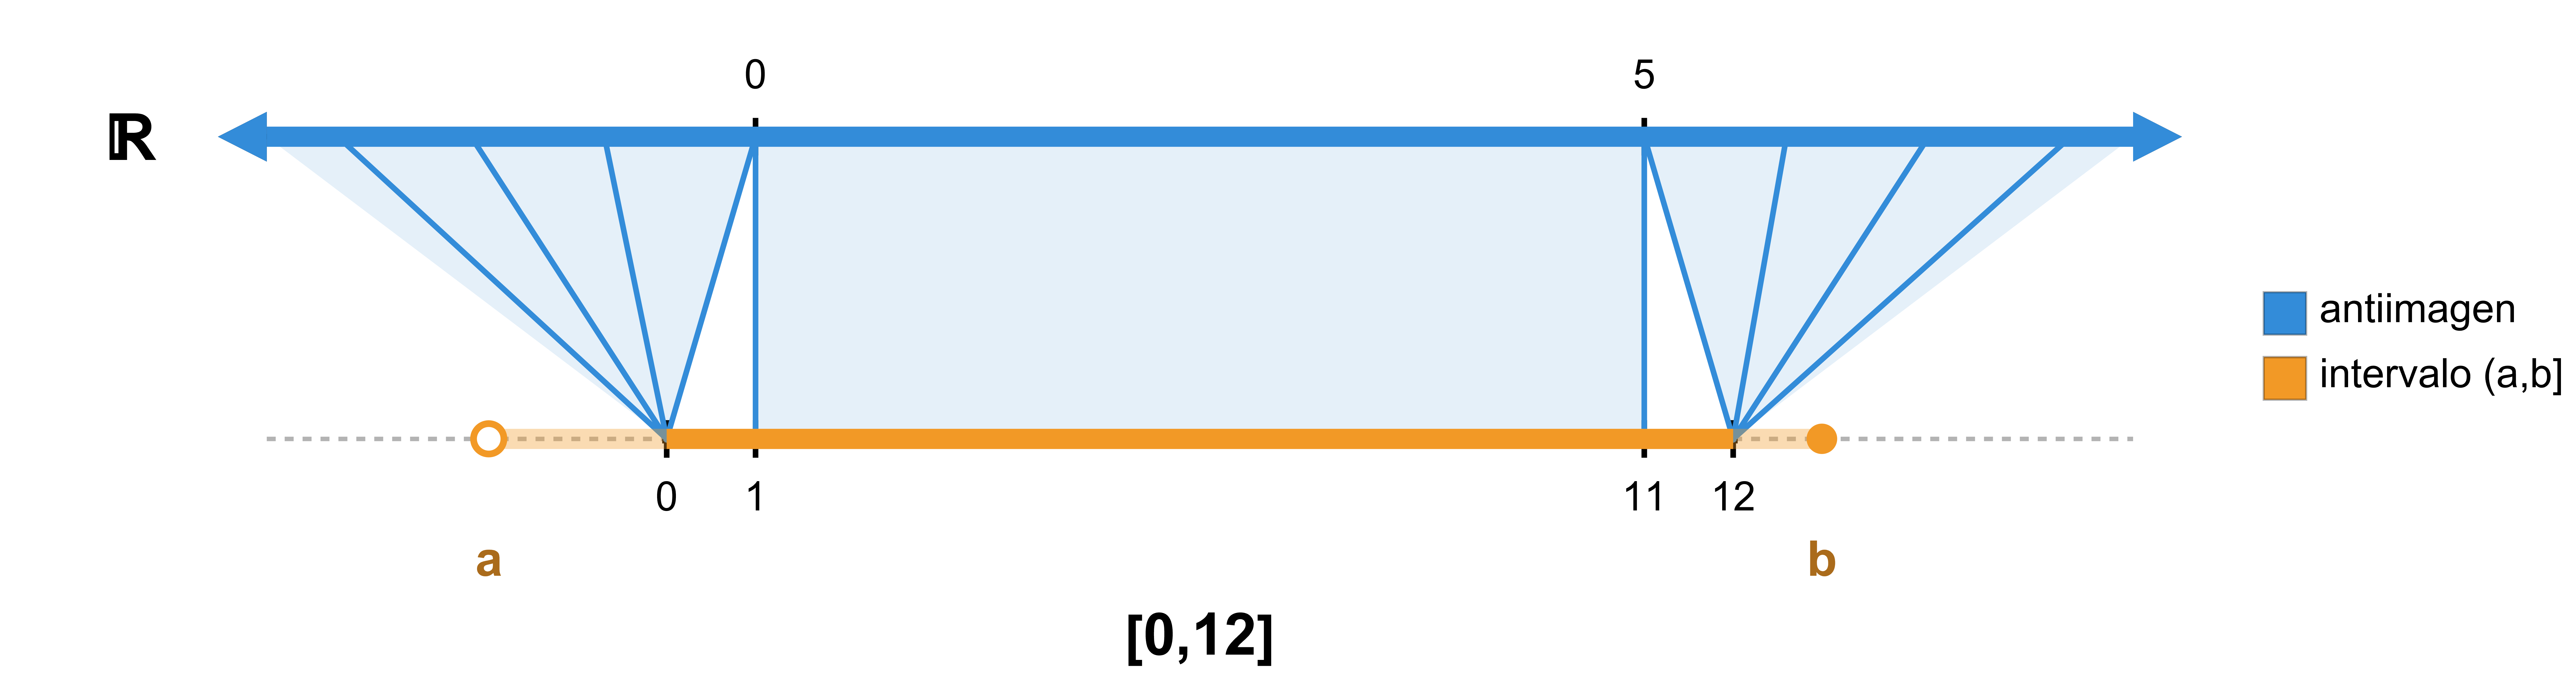
\includegraphics[width=0.75\linewidth]{imagenes/tema3/T3_P49_c05.png}
    \end{center}
\end{itemize}

\newpage
\paragraph{2. Casos con $0 \le a < 1$ (la traza no contiene al $0$ ni al $1$):}
\begin{itemize}
    \item \textbf{Caso 6 ($a < b < 1$):} $(a,b] \cap \mathrm{Im}(f) = \varnothing \implies f^{-1}(\varnothing) = \varnothing \in \mathcal{B}$.
    \begin{center}
        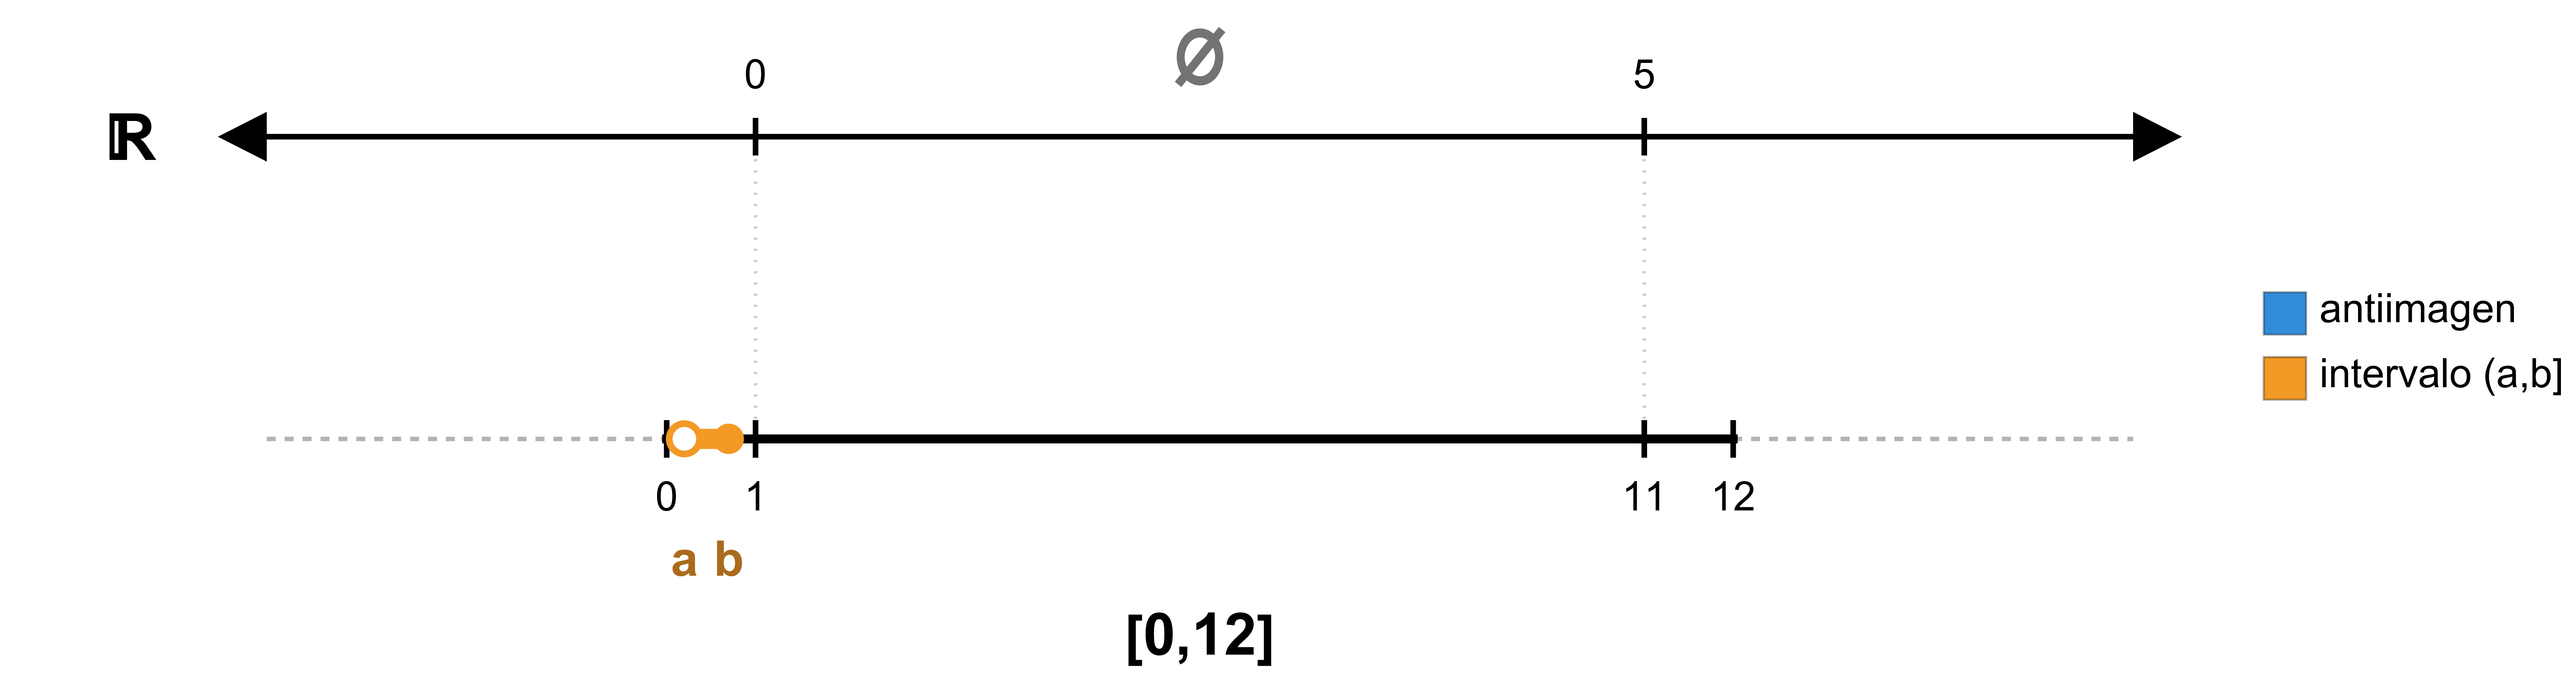
\includegraphics[width=0.75\linewidth]{imagenes/tema3/T3_P49_c06.png}
    \end{center}

    \item \textbf{Caso 7 ($1 \le b < 11$):} $(a,b] \cap \mathrm{Im}(f) = [1,b] \implies f^{-1}([1,b]) = \left[0, \frac{b-1}{2}\right] \in \mathcal{B}$.
    \begin{center}
        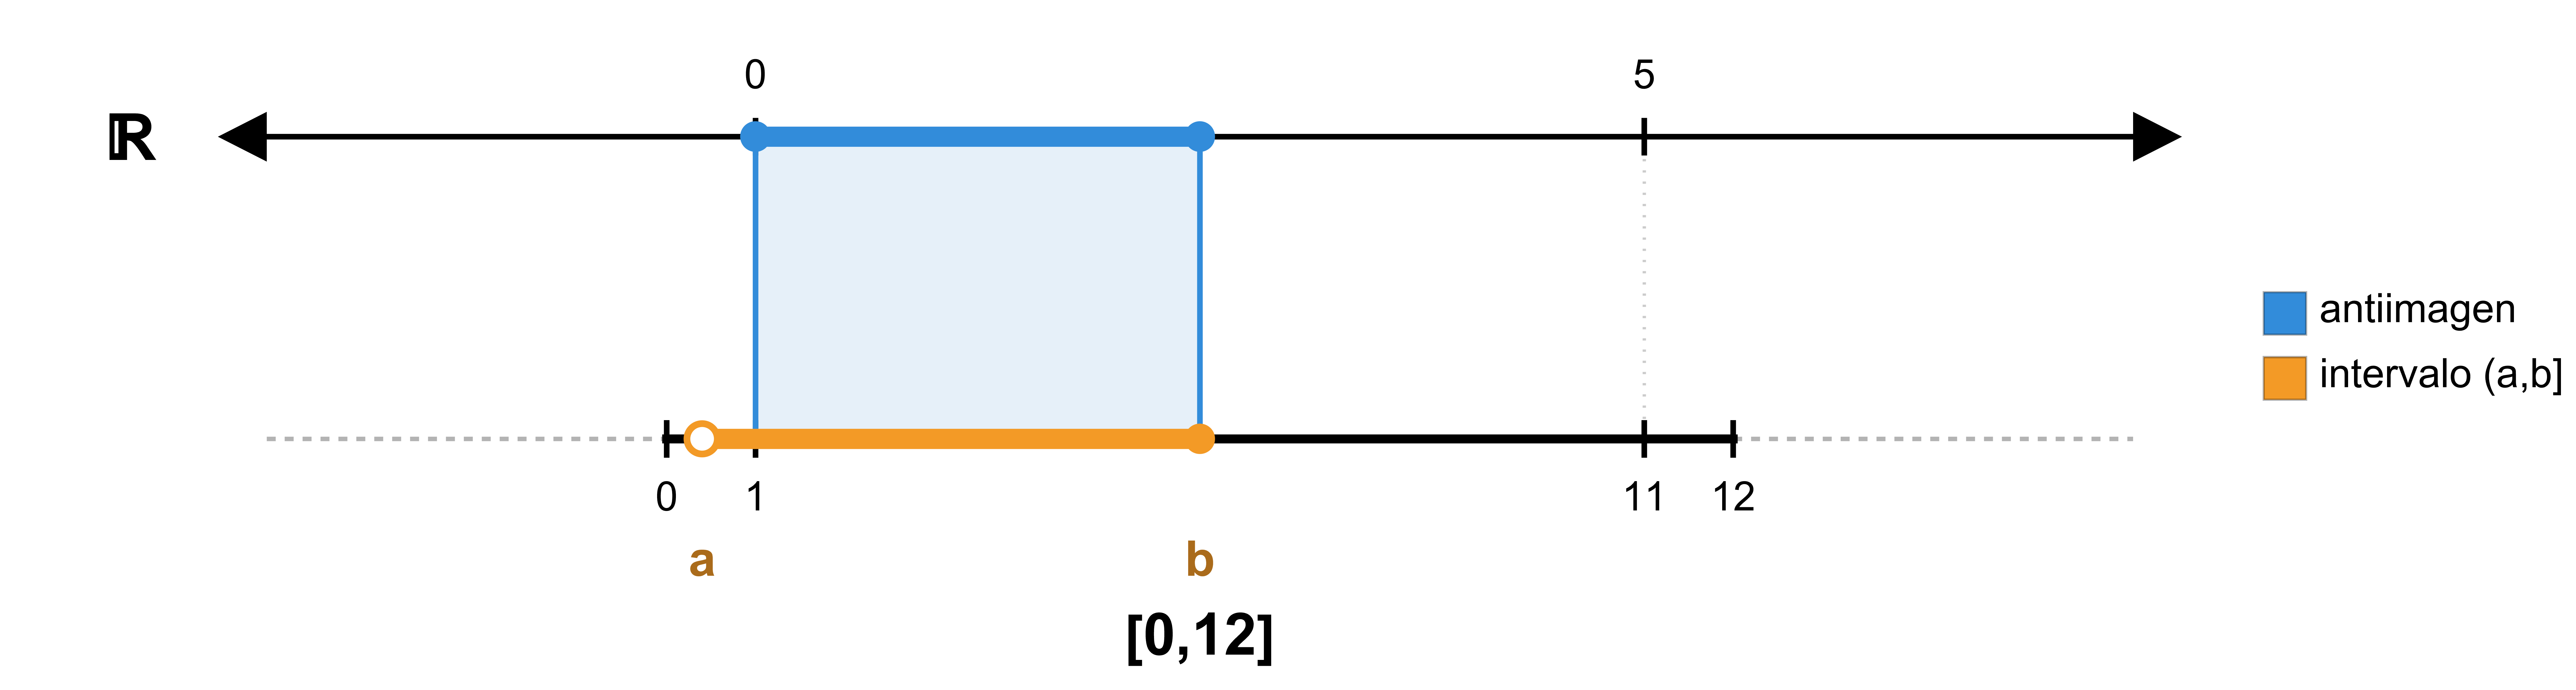
\includegraphics[width=0.75\linewidth]{imagenes/tema3/T3_P49_c07.png}
    \end{center}

    \item \textbf{Caso 8 ($11 \le b < 12$):} $(a,b] \cap \mathrm{Im}(f) = [1,11) \implies f^{-1}([1,11)) = [0, 5) \in \mathcal{B}$.
    \begin{center}
        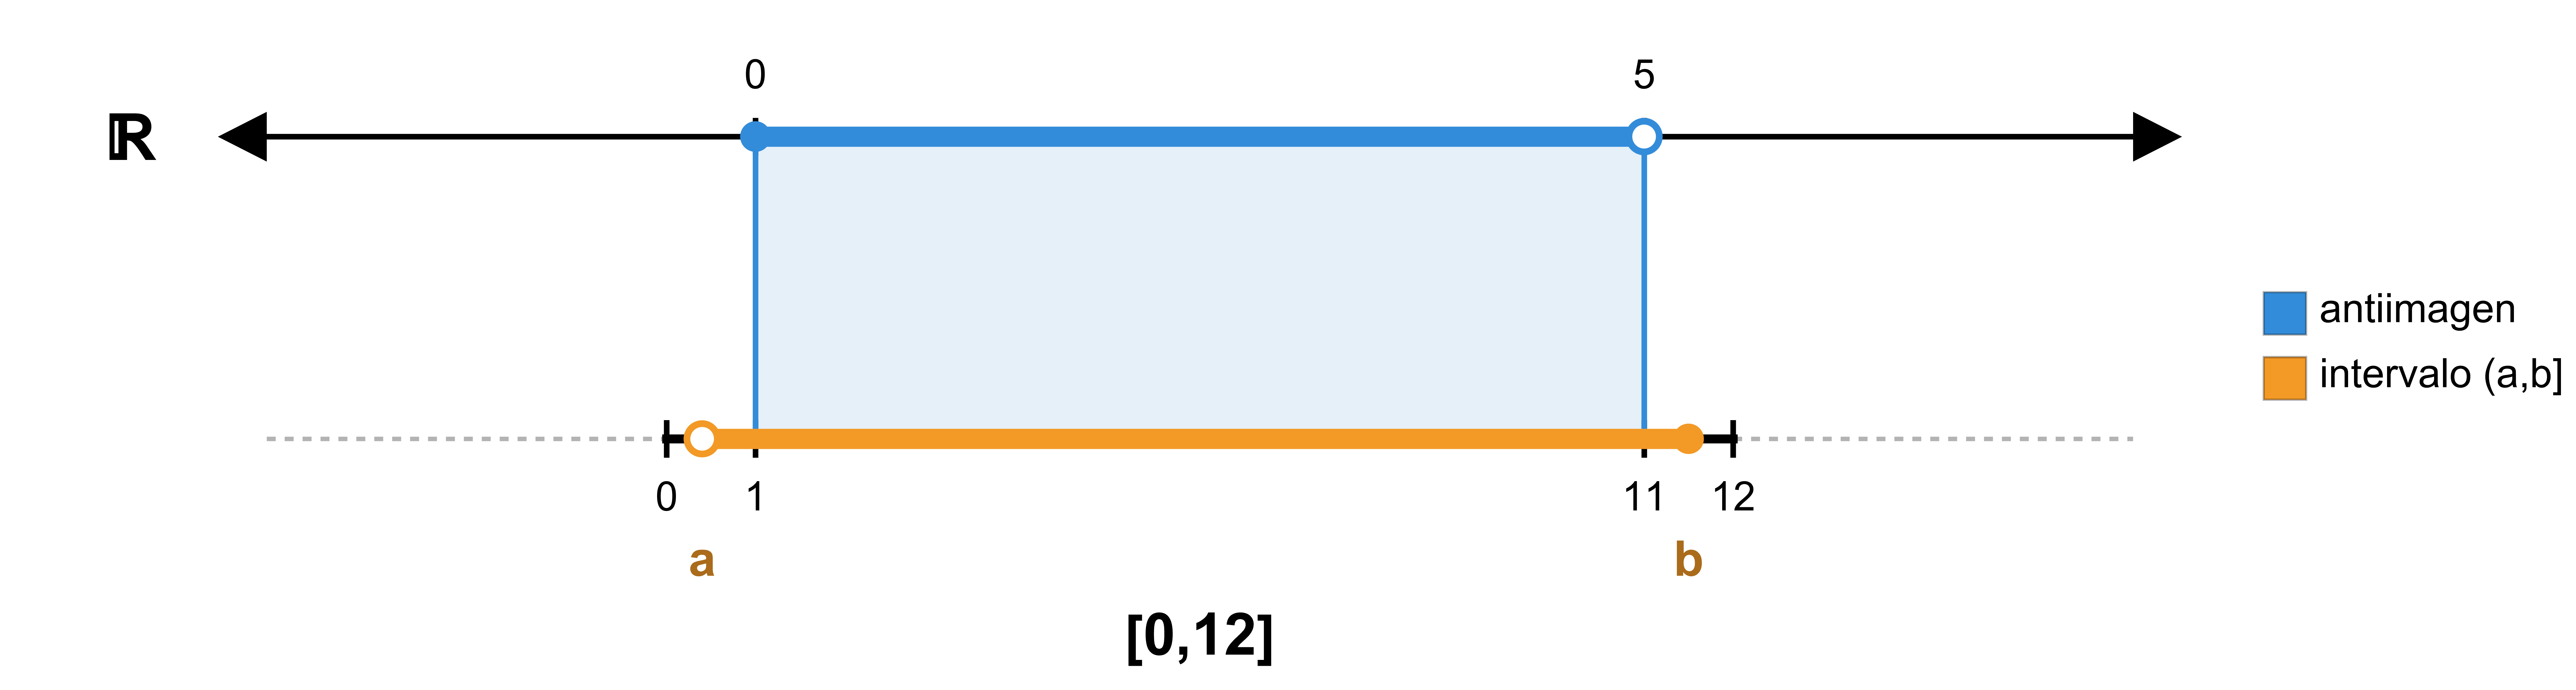
\includegraphics[width=0.75\linewidth]{imagenes/tema3/T3_P49_c08.png}
    \end{center}

    \item \textbf{Caso 9 ($b \ge 12$):} $(a,12] \cap \mathrm{Im}(f) = [1,11) \cup \{12\} \implies \\
    \implies f^{-1}([1,11)) \cup f^{-1}(\{12\}) = [0, 5) \cup [5, \infty) = [0, \infty) \in \mathcal{B}$.
    \begin{center}
        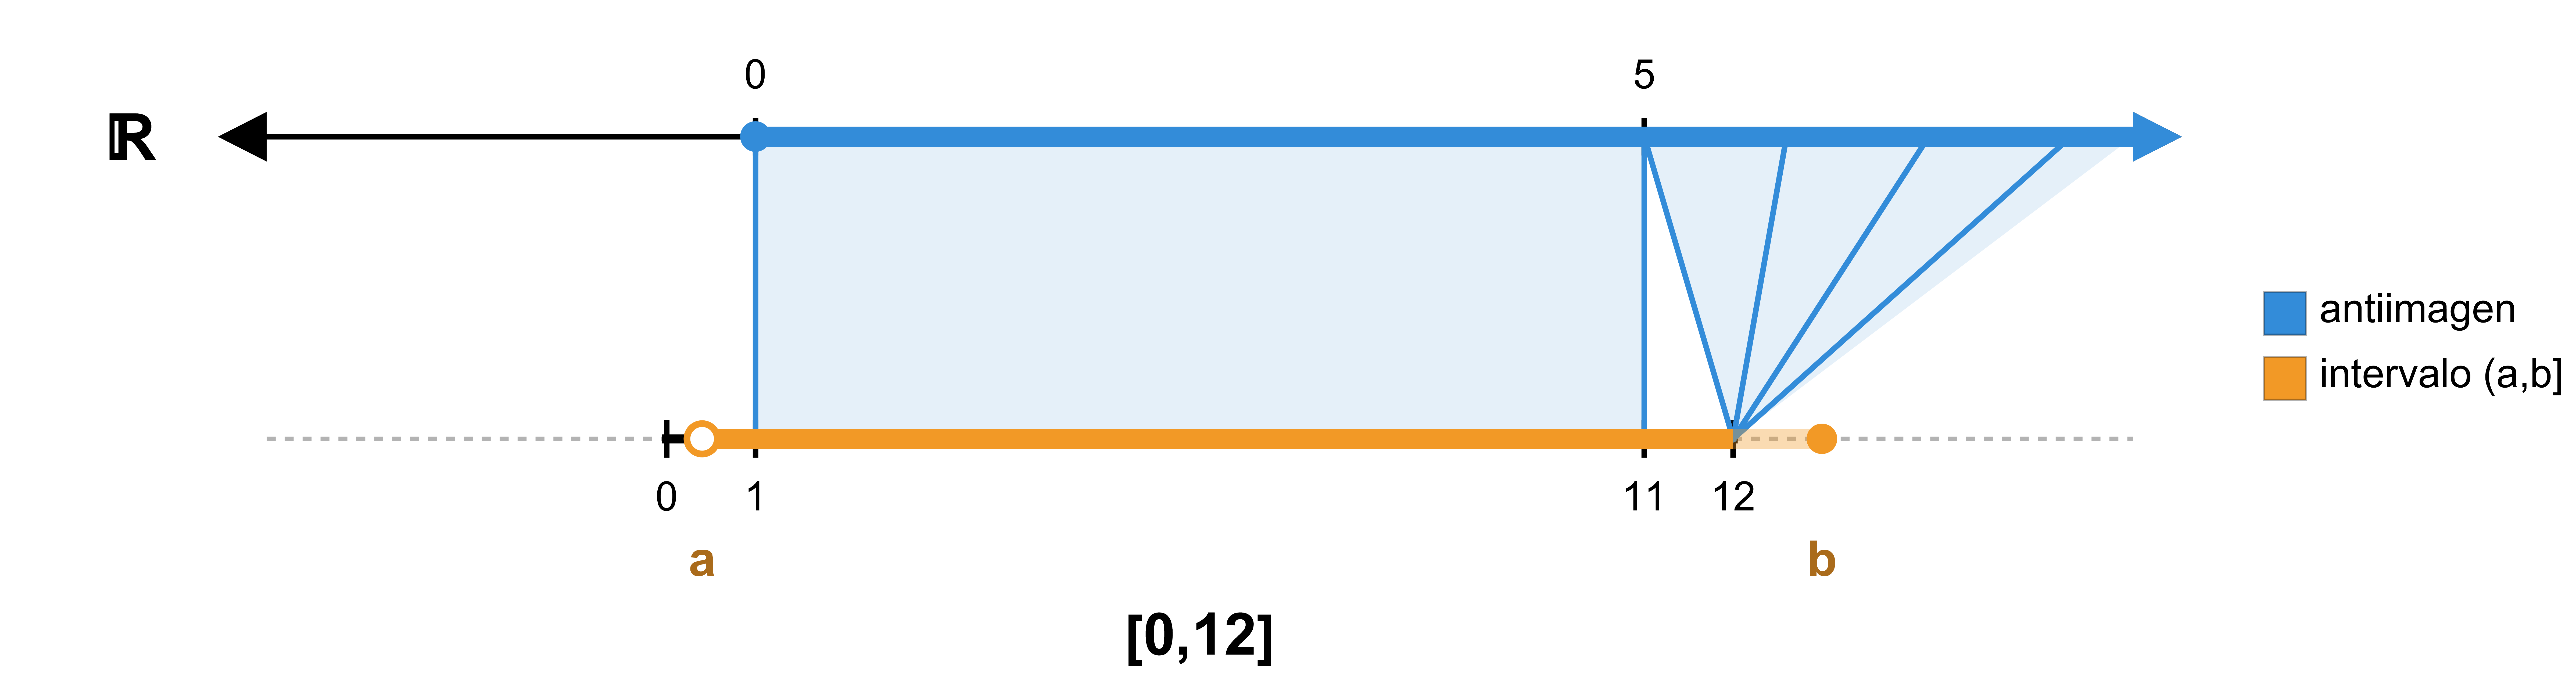
\includegraphics[width=0.75\linewidth]{imagenes/tema3/T3_P49_c09.png}
    \end{center}
\end{itemize}

\paragraph{3. Casos con $1 \le a < 11$ (la traza intersecta el tramo continuo $[1, 11)$):}
\begin{itemize}
    \item \textbf{Caso 10 ($a < b < 11$):} $(a,b] \cap \mathrm{Im}(f) = (a,b] \implies f^{-1}((a,b]) = \left(\frac{a-1}{2}, \frac{b-1}{2}\right] \in \mathcal{B}$.
    \begin{center}
        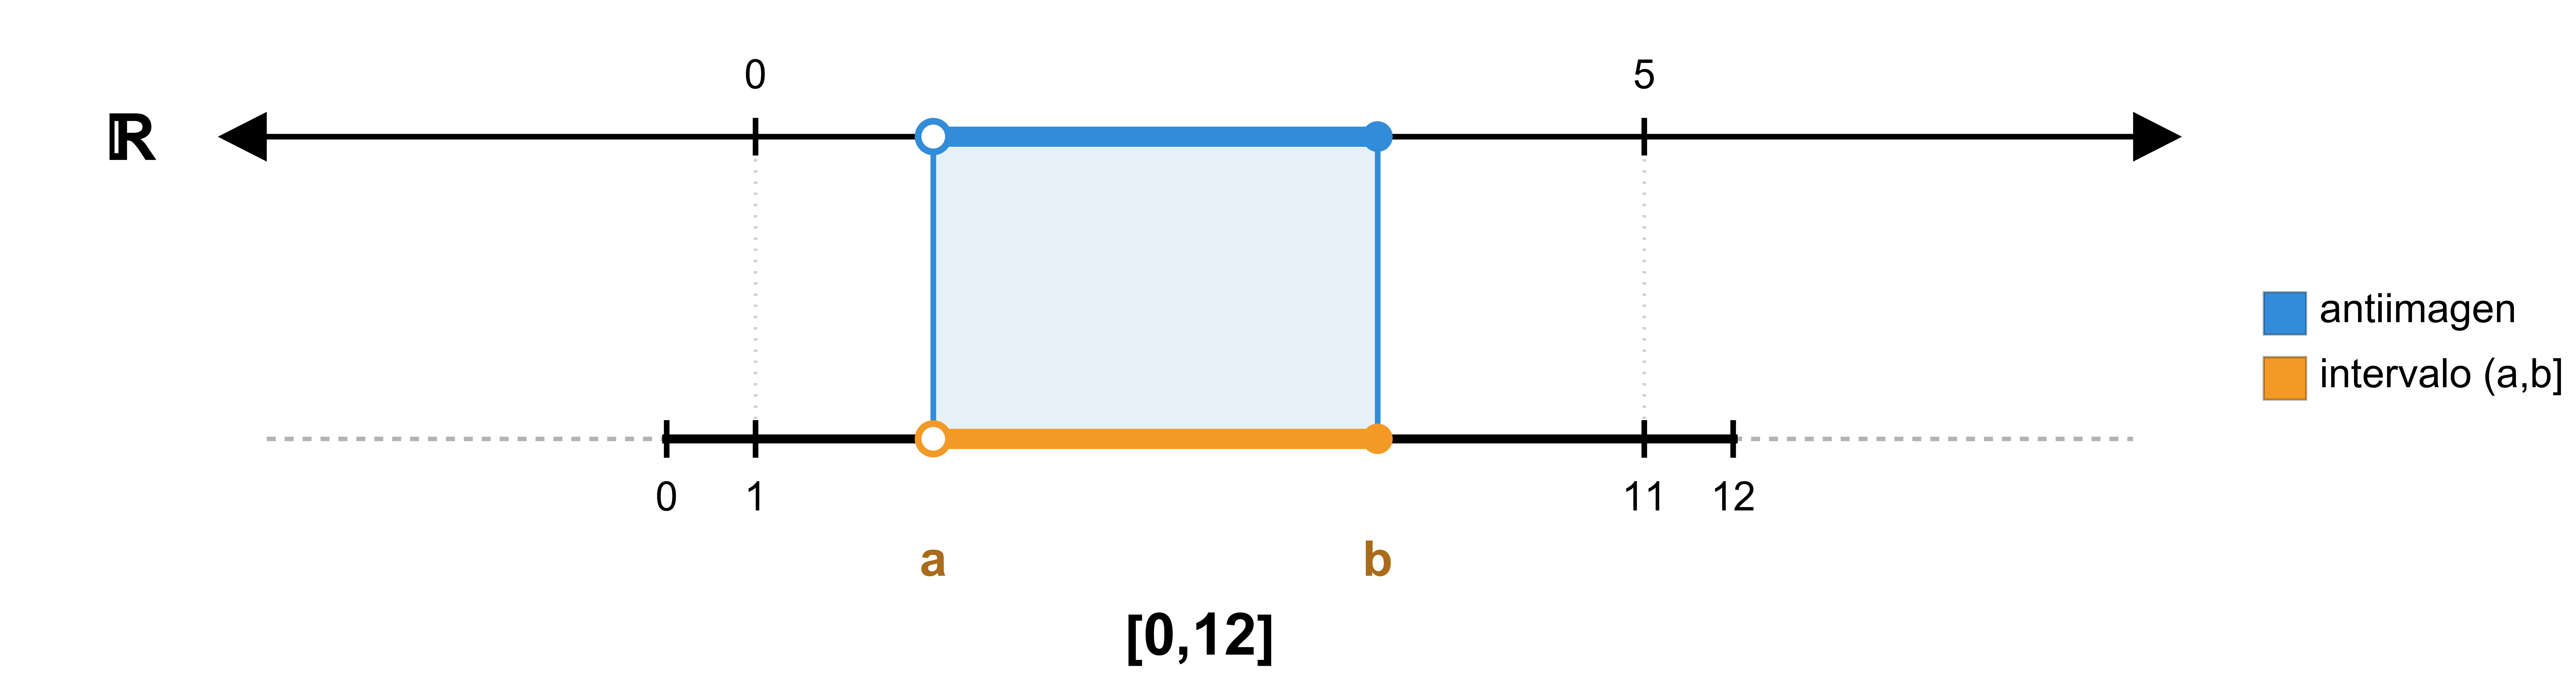
\includegraphics[width=0.75\linewidth]{imagenes/tema3/T3_P49_c10.png}
    \end{center}

    \newpage
    \item \textbf{Caso 11 ($11 \le b < 12$):} $(a,b] \cap \mathrm{Im}(f) = (a,11) \implies f^{-1}((a,11)) = \left(\frac{a-1}{2}, 5\right) \in \mathcal{B}$.
    \begin{center}
        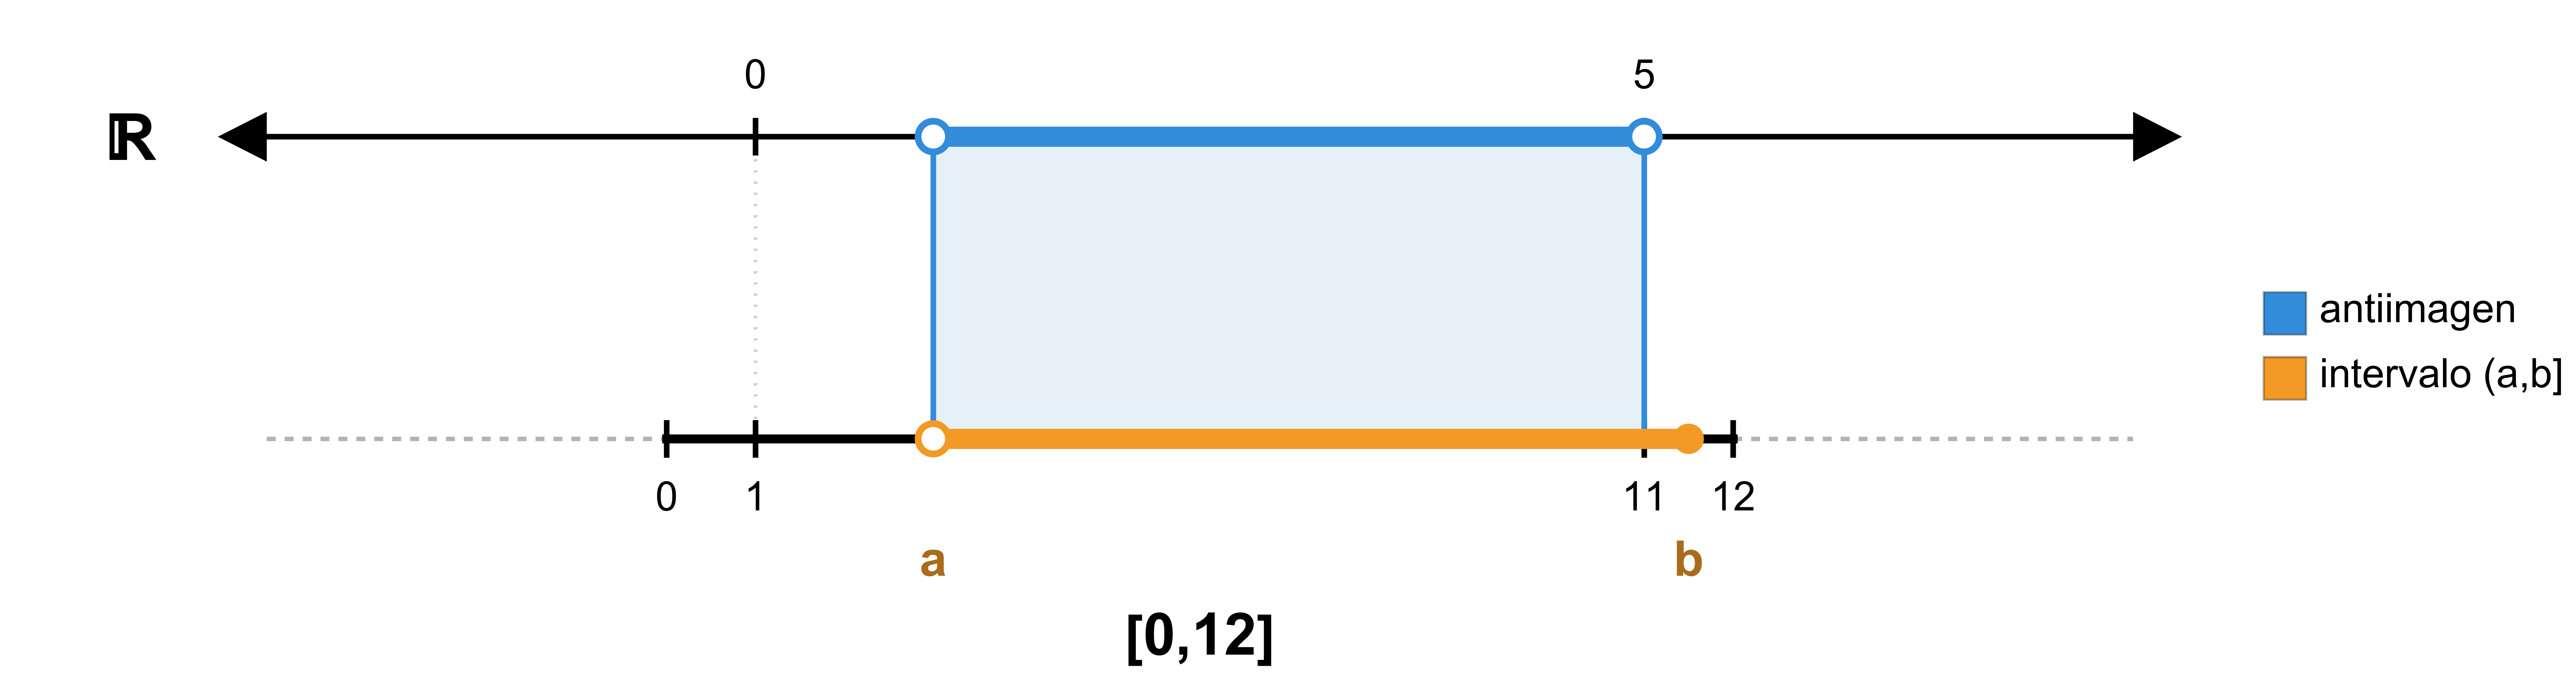
\includegraphics[width=0.75\linewidth]{imagenes/tema3/T3_P49_c11.png}
    \end{center}

    \item \textbf{Caso 12 ($b \ge 12$):} $(a,12] \cap \mathrm{Im}(f) = (a,11) \cup \{12\} \implies \\
    \implies f^{-1}((a,11)) \cup f^{-1}(\{12\}) = \left(\frac{a-1}{2}, 5\right) \cup [5, \infty) = \left(\frac{a-1}{2}, \infty\right) \in \mathcal{B}$.
    \begin{center}
        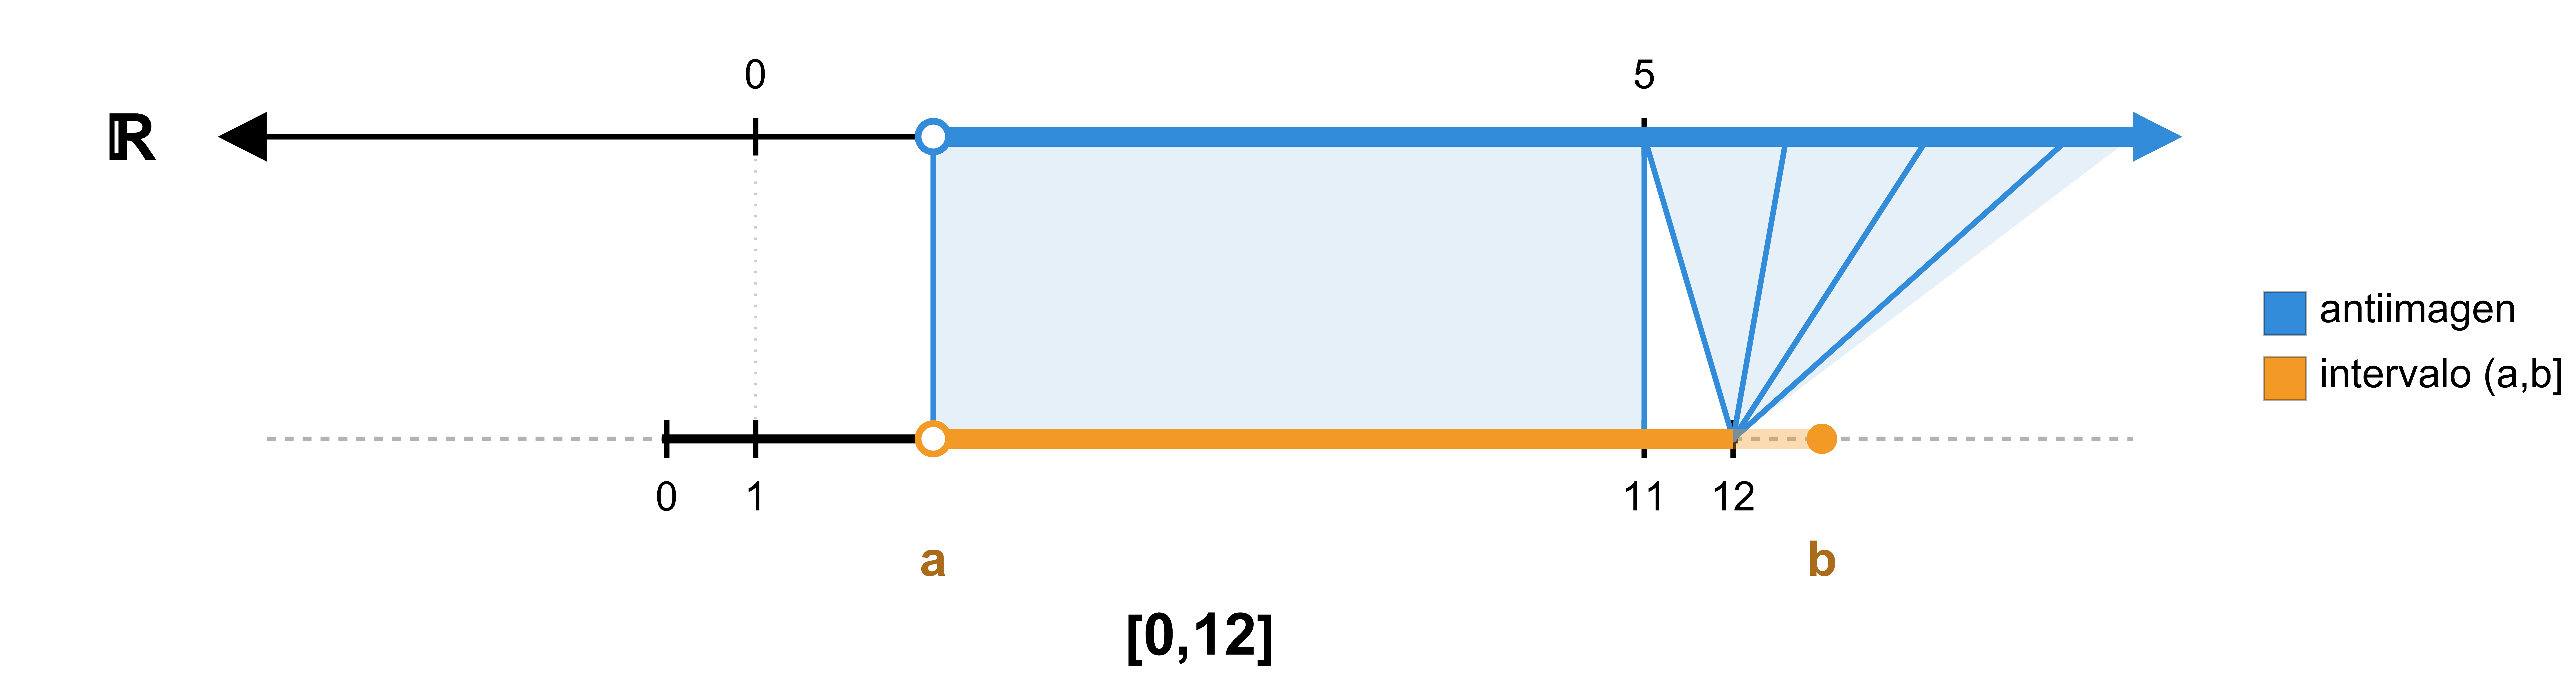
\includegraphics[width=0.75\linewidth]{imagenes/tema3/T3_P49_c12.png}
    \end{center}
\end{itemize}

\paragraph{4. Casos con $a \ge 11$ (la traza cae a la derecha de la discontinuidad):}
\begin{itemize}
    \item \textbf{Caso 13 ($11 \le a < b < 12$):} $(a,b] \cap \mathrm{Im}(f) = \varnothing \implies f^{-1}(\varnothing) = \varnothing \in \mathcal{B}$.
    \begin{center}
        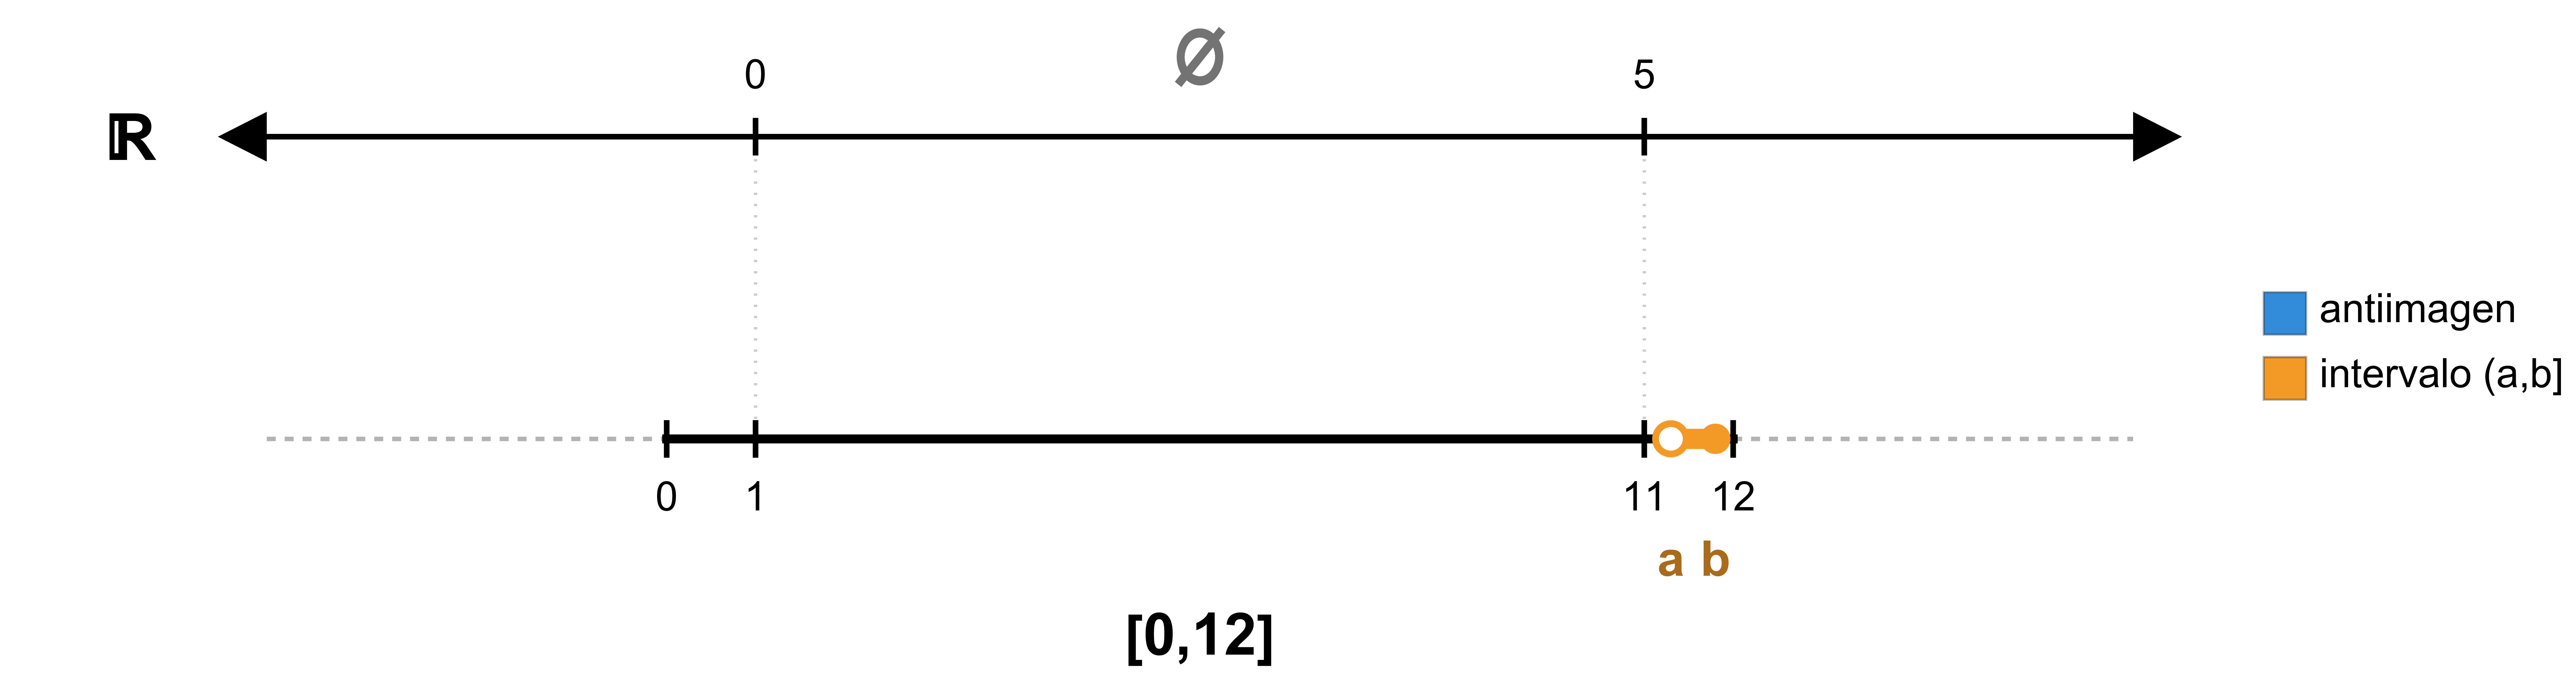
\includegraphics[width=0.75\linewidth]{imagenes/tema3/T3_P49_c13.png}
    \end{center}

    \item \textbf{Caso 14 ($11 \le a < 12 \le b$):} $(a,b] \cap [0,12] = (a, 12]$, luego\\ $(a,12] \cap \mathrm{Im}(f) = \{12\} \implies f^{-1}(\{12\}) = [5, \infty) \in \mathcal{B}$.
    \begin{center}
        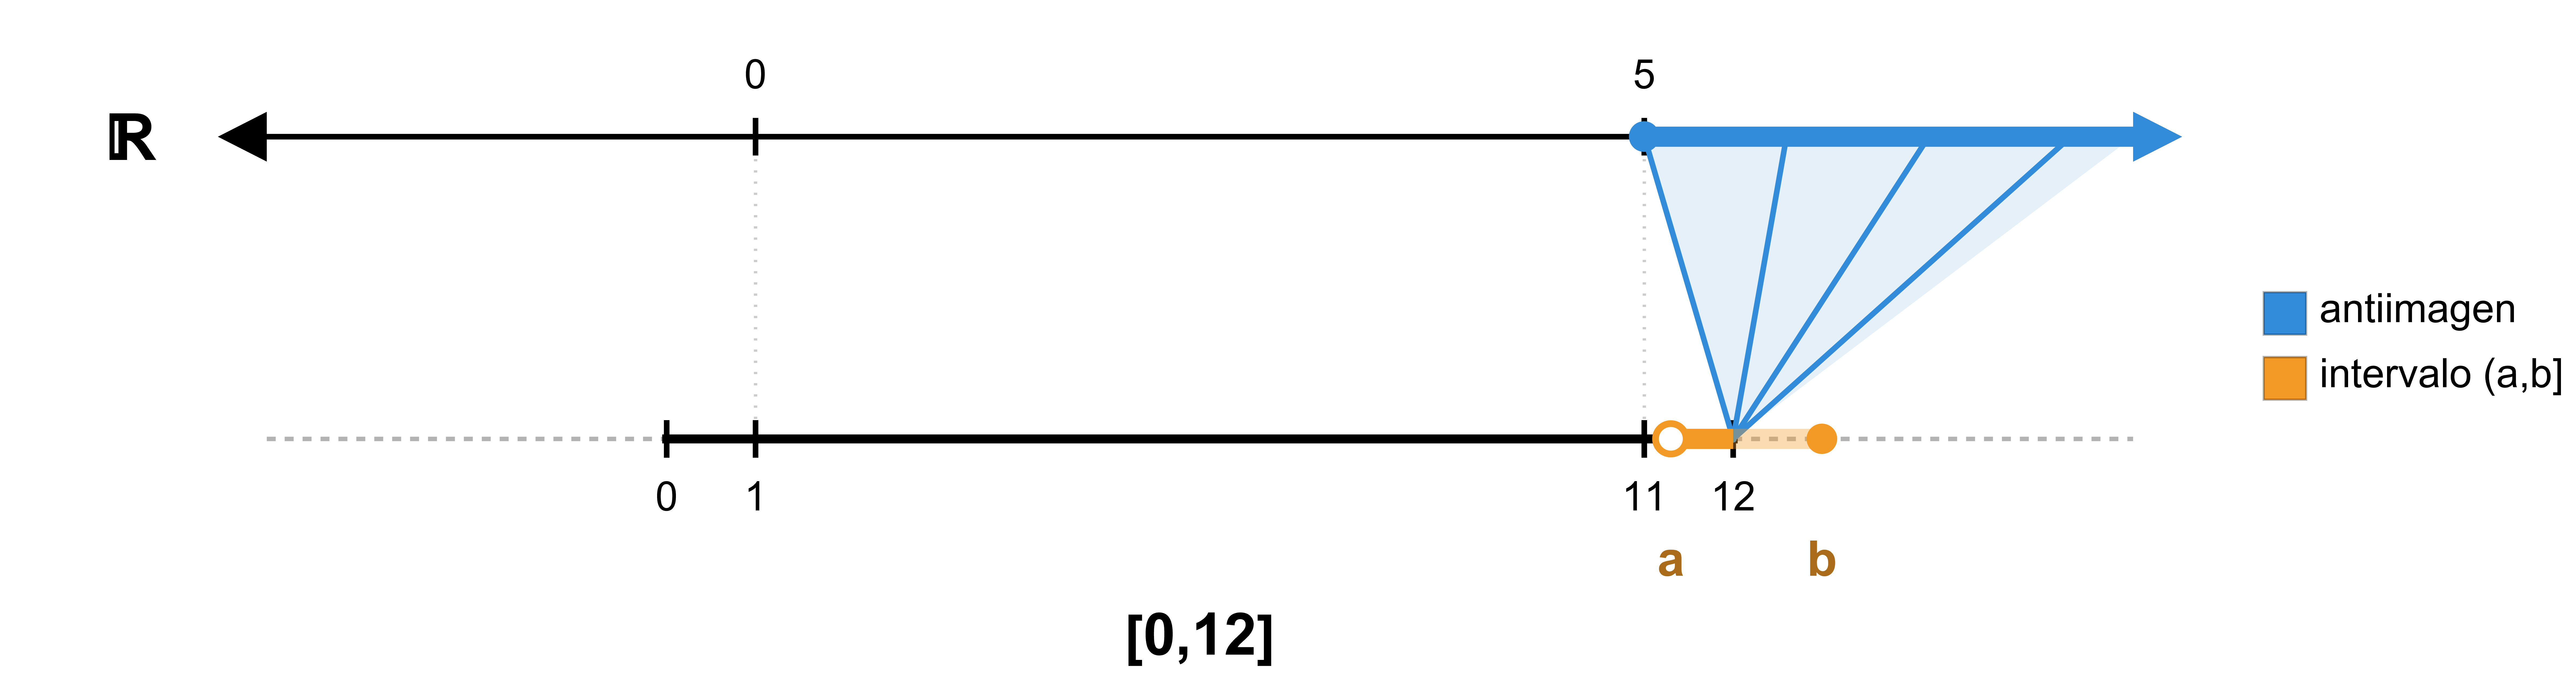
\includegraphics[width=0.75\linewidth]{imagenes/tema3/T3_P49_c14.png}
    \end{center}

    \item \textbf{Caso 15 ($a \ge 12$):} $(a,b] \cap [0,12] = \varnothing \implies f^{-1}(\varnothing) = \varnothing \in \mathcal{B}$.
    \begin{center}
        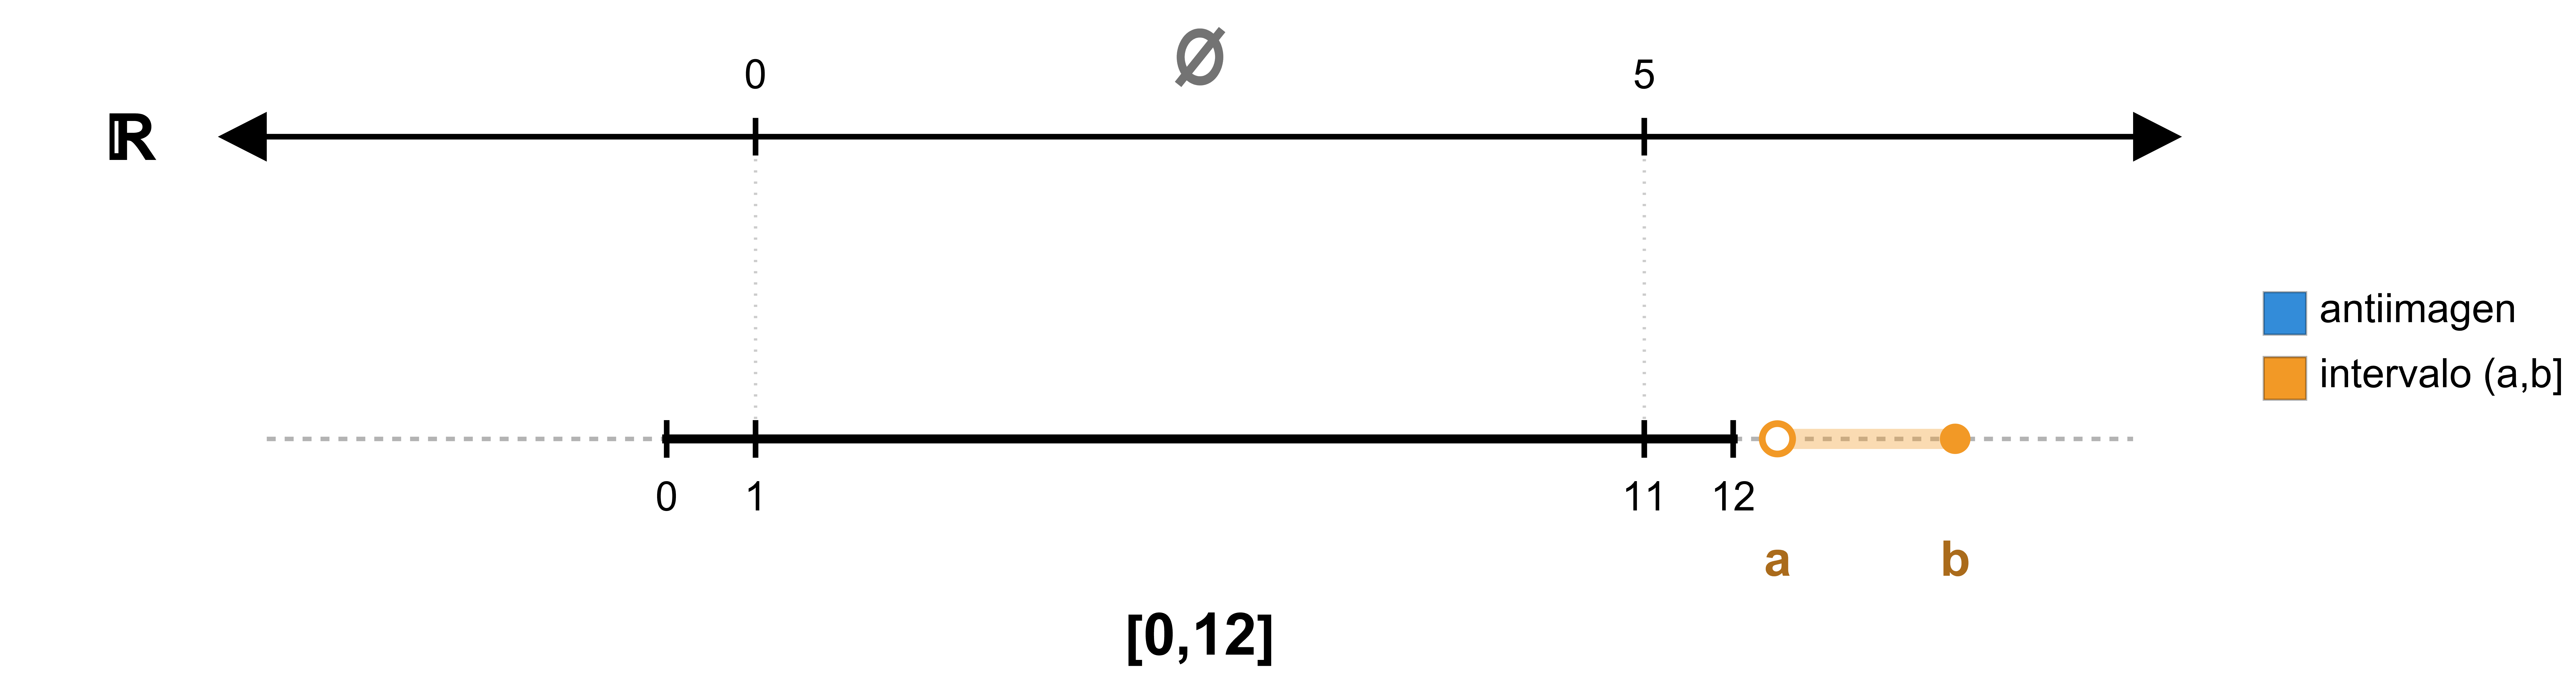
\includegraphics[width=0.75\linewidth]{imagenes/tema3/T3_P49_c15.png}
    \end{center}
\end{itemize}

Puesto que en los 15 casos exhaustivos la imagen inversa $f^{-1}((a,b] \cap [0,12])$ resulta ser siempre un conjunto boreliano ($f^{-1}(I) \in \mathcal{B}$), queda demostrado que la función $f$ es medible.
\end{problema}

\newpage
%===================
% Problema 50: 
%===================
\begin{problema}[Medibilidad y medida inducida por una función definida a trozos]
Sea $\lambda$ la medida de Lebesgue sobre el espacio medible $([0, 1], \mathcal{B}_{[0,1]})$ y consideremos la medida $\mu = 2\lambda$. Se define la aplicación $f : ([0, 1], \mathcal{B}_{[0,1]}, \mu) \to ([0, 2], \mathcal{B}_{[0,2]})$ por:
\[
    f(\omega) = \begin{cases}
        0 & \text{si } 0 \le \omega < \frac{t}{2} \\[4pt]
        \omega + \frac{t}{2} & \text{si } \frac{t}{2} \le \omega < t \\[4pt]
        \frac{3}{4} & \text{si } t \le \omega \le \frac{3}{4} \\[4pt]
        2\omega & \text{si } \frac{3}{4} < \omega \le 1
    \end{cases}
\]
donde $t \in \left(0, \frac{1}{2}\right)$ es un parámetro fijo.
\begin{enumerate}[label=\alph*)]
    \item Demostrar que la función $f$ es medible.
    \item Hallar la expresión general de la medida inducida $\mu_f = \mu \circ f^{-1}$ sobre la clase generadora de semirrectas $[0, x]$ con $x \in [0, 2]$.
    \item Para el caso particular $t = \frac{1}{4}$, calcular las medidas $\mu_f([0, 1])$, $\mu_f\left(\left[0, \frac{3}{4}\right]\right)$, $\mu_f\left(\left[0, \frac{3}{4}\right)\right)$, $\mu_f\left(\left\{\frac{3}{4}\right\}\right)$ y $\mu_f\left(\left[0, \frac{3}{8}\right)\right)$.
\end{enumerate}

\tcblower

\textbf{a) Demostración de la medibilidad de $f$:}

Para probar la medibilidad de $f$, utilizaremos la clase generadora $\mathcal{C} = \{[0, x] \mid x \in [0, 2]\}$, la cual genera la $\sigma$-álgebra de Borel $\mathcal{B}_{[0,2]}$.

Analizamos la imagen directa de $f$, dada por $\mathrm{Im}(f) = \{0\} \cup \left[t, \frac{3t}{2}\right) \cup \left\{\frac{3}{4}\right\} \cup \left(\frac{3}{2}, 2\right]$. Calculamos la antiimagen $f^{-1}([0, x])$ según el valor del parámetro $x \in [0, 2]$:

\begin{itemize}
    \item \textbf{Si $0 \le x < t$:}
    Únicamente el valor $0 \in \mathrm{Im}(f)$ pertenece al intervalo $[0, x]$. Como $f(\omega) = 0 \iff 0 \le \omega < \frac{t}{2}$:
    \[
        f^{-1}([0, x]) = \left[0, \frac{t}{2}\right) \in \mathcal{B}_{[0,1]}
    \]

    \item \textbf{Si $t \le x < \frac{3t}{2}$:}
    El intervalo $[0, x]$ contiene al valor $0$ y al tramo lineal $\omega + \frac{t}{2} \le x \iff \omega \le x - \frac{t}{2}$. Uniendo ambos tramos obtenemos:
    \[
        f^{-1}([0, x]) = \left[0, \frac{t}{2}\right) \cup \left[\frac{t}{2}, x - \frac{t}{2}\right] = \left[0, x - \frac{t}{2}\right] \in \mathcal{B}_{[0,1]}
    \]

    \item \textbf{Si $\frac{3t}{2} \le x < \frac{3}{4}$:}
    El intervalo $[0, x]$ contiene a $0$ y a todo el tramo continuo $\left[t, \frac{3t}{2}\right)$, pero no al punto $\frac{3}{4}$. Por tanto:
    \[
        f^{-1}([0, x]) = [0, t) \in \mathcal{B}_{[0,1]}
    \]

    \item \textbf{Si $\frac{3}{4} \le x \le \frac{3}{2}$:}
    El intervalo $[0, x]$ contiene a $0$, a $\left[t, \frac{3t}{2}\right)$ y al punto $\frac{3}{4}$ (cuya antiimagen es $\left[t, \frac{3}{4}\right]$):
    \[
        f^{-1}([0, x]) = [0, t) \cup \left[t, \frac{3}{4}\right] = \left[0, \frac{3}{4}\right] \in \mathcal{B}_{[0,1]}
    \]

    \item \textbf{Si $\frac{3}{2} < x \le 2$:}
    El intervalo $[0, x]$ incluye además la región $2\omega \le x \iff \omega \le \frac{x}{2}$. Como $x > \frac{3}{2} \implies \frac{x}{2} > \frac{3}{4}$:
    \[
        f^{-1}([0, x]) = \left[0, \frac{3}{4}\right] \cup \left(\frac{3}{4}, \frac{x}{2}\right] = \left[0, \frac{x}{2}\right] \in \mathcal{B}_{[0,1]}
    \]
\end{itemize}

Dado que la antiimagen de todo intervalo de la clase generadora es un conjunto boreliano de $[0, 1]$, se concluye que \textbf{$f$ es una función medible}.

% Espacio reservado para incorporar diagrama explicativo en los apuntes
\begin{center}
    \vspace{0.2cm}
    \framebox[\linewidth]{\vbox to 2.2cm{\vfill \centering \textit{[Espacio reservado para diagrama: Gráfica de la función $f(\omega)$ con sus tramos constantes y lineales, ilustrando las antiimágenes $f^{-1}([0, x])$]} \vfill}}
    \vspace{0.2cm}
\end{center}

\textbf{b) Expresión general de la medida inducida $\mu_f([0, x])$:}

Aplicando la definición $\mu_f([0, x]) = \mu(f^{-1}([0, x])) = 2\lambda(f^{-1}([0, x]))$, evaluamos el doble de la longitud de Lebesgue de los intervalos obtenidos en el apartado anterior:
\[
    \mu_f([0, x]) = \begin{cases}
        2 \cdot \frac{t}{2} = t & \text{si } 0 \le x < t \\[4pt]
        2 \left(x - \frac{t}{2}\right) = 2x - t & \text{si } t \le x < \frac{3t}{2} \\[4pt]
        2 \cdot t = 2t & \text{si } \frac{3t}{2} \le x < \frac{3}{4} \\[4pt]
        2 \cdot \frac{3}{4} = \frac{3}{2} & \text{si } \frac{3}{4} \le x \le \frac{3}{2} \\[4pt]
        2 \cdot \frac{x}{2} = x & \text{si } \frac{3}{2} < x \le 2
    \end{cases}
\]

\textbf{c) Particularización para $t = \frac{1}{4}$ y cálculo de medidas específicas:}

Sustituyendo $t = \frac{1}{4}$ (con lo que $\frac{3t}{2} = \frac{3}{8}$), la función de distribución acumulada de la medida inducida queda:
\[
    \mu_f([0, x]) = \begin{cases}
        \frac{1}{4} & \text{si } 0 \le x < \frac{1}{4} \\[4pt]
        2x - \frac{1}{4} & \text{si } \frac{1}{4} \le x < \frac{3}{8} \\[4pt]
        \frac{1}{2} & \text{si } \frac{3}{8} \le x < \frac{3}{4} \\[4pt]
        \frac{3}{2} & \text{si } \frac{3}{4} \le x \le \frac{3}{2} \\[4pt]
        x & \text{si } \frac{3}{2} < x \le 2
    \end{cases}
\]

Calculamos cada una de las medidas solicitadas:
\begin{enumerate}[label=\arabic*.]
    \item \textbf{$\mu_f([0, 1])$:}
    Como $x = 1 \in \left[\frac{3}{4}, \frac{3}{2}\right]$, evaluamos directamente en dicha rama:
    \[
        \mu_f([0, 1]) = \frac{3}{2}
    \]

    \item \textbf{$\mu_f\left(\left[0, \frac{3}{4}\right]\right)$:}
    Evaluando en $x = \frac{3}{4}$:
    \[
        \mu_f\left(\left[0, \frac{3}{4}\right]\right) = \frac{3}{2}
    \]

    \item \textbf{$\mu_f\left(\left[0, \frac{3}{4}\right)\right)$:}
    Tomando el límite por la izquierda cuando $x \to \left(\frac{3}{4}\right)^-$ sobre la rama $\frac{3}{8} \le x < \frac{3}{4}$:
    \[
        \mu_f\left(\left[0, \frac{3}{4}\right)\right) = \lim_{x \to (3/4)^-} \mu_f([0, x]) = \frac{1}{2}
    \]

    \item \textbf{$\mu_f\left(\left\{\frac{3}{4}\right\}\right)$:}
    Por la propiedad del salto puntual de la medida inducida:
    \[
        \mu_f\left(\left\{\frac{3}{4}\right\}\right) = \mu_f\left(\left[0, \frac{3}{4}\right]\right) - \mu_f\left(\left[0, \frac{3}{4}\right)\right) = \frac{3}{2} - \frac{1}{2} = 1
    \]
    \textit{Comprobación directa:} $f^{-1}\left(\left\{\frac{3}{4}\right\}\right) = \left[\frac{1}{4}, \frac{3}{4}\right] \implies \mu\left(\left[\frac{1}{4}, \frac{3}{4}\right]\right) = 2 \left(\frac{3}{4} - \frac{1}{4}\right) = 1$.

    \item \textbf{$\mu_f\left(\left[0, \frac{3}{8}\right)\right)$:}
    Tomando el límite por la izquierda cuando $x \to \left(\frac{3}{8}\right)^-$ en la rama $2x - \frac{1}{4}$:
    \[
        \mu_f\left(\left[0, \frac{3}{8}\right)\right) = \lim_{x \to (3/8)^-} \left(2x - \frac{1}{4}\right) = 2 \left(\frac{3}{8}\right) - \frac{1}{4} = \frac{3}{4} - \frac{1}{4} = \frac{1}{2}
    \]
\end{enumerate}
\end{problema}